% UCL Thesis LaTeX Template
%  (c) Ian Kirker, 2014
% 
% Note that the \input command just streams in whatever file you give
%  it, while the \include command adds a page break, and does some
%  extra organisation to make compilation faster. Note that you can't
%  use \include inside an \include-d file.
% We suggest using \input for settings and configuration files that
%  you always want to use, and \include for each section of content.
% If you do that, it also means you can use the \includeonly statement
%  to only compile up the section you're currently interested in.
% You might also want to put figures into their own files to be \input.

% For more information on \input and \include, see:
%  http://tex.stackexchange.com/questions/246/when-should-i-use-input-vs-include


% Formatting and binding rules for theses are here: 
%  https://www.ucl.ac.uk/students/exams-and-assessments/research-assessments/format-bind-and-submit-your-thesis-general-guidance

% This package goes first and foremost, because it checks all 
%  your syntax for mistakes and some old-fashioned LaTeX commands.
% Note that normally you should load your documentclass before 
%  packages, because some packages change behaviour based on
%  your document settings.
% Also, for those confused by the RequirePackage here vs usepackage
%  elsewhere, usepackage cannot be used before the documentclass
%  command, while RequirePackage can. That's the only functional
%  difference as far as I'm aware.
\RequirePackage[l2tabu, orthodox]{nag}


% ------ Main document class specification ------
% The draft option here prevents images being inserted,
%  and adds chunky black bars to boxes that are exceeding 
%  the page width (to show that they are).
% The oneside option can optionally be replaced by twoside if
%  you intend to print double-sided. Note that this is
%  *specifically permitted* by the UCL thesis formatting
%  guidelines.
%
% Valid options in terms of type are:
%  phd
%  mres
%  mphil
%\documentclass[12pt,phd,draft,a4paper,oneside]{ucl_thesis}
\documentclass[12pt,phd,a4paper,oneside]{ucl_thesis}




% Package configuration:
%  LaTeX uses "packages" to add extra commands and features.
%  There are quite a few useful ones, so we've put them in a 

%   separate file.
% -------- Packages --------

% This package just gives you a quick way to dump in some sample text.
% You can remove it -- it's just here for the examples.
\usepackage{blindtext}

% This package means empty pages (pages with no text) won't get stuff
%  like chapter names at the top of the page. It's mostly cosmetic.
\usepackage{emptypage}

% The graphicx package adds the \includegraphics command,
%  which is your basic command for adding a picture.
\usepackage{graphicx}

% The float package improves LaTeX's handling of floats,
%  and also adds the option to *force* LaTeX to put the float
%  HERE, with the [H] option to the float environment.
\usepackage{float}

% The amsmath package enhances the various ways of including
%  maths, including adding the align environment for aligned
%  equations.
\usepackage{amsmath}

% Use these two packages together -- they define symbols
%  for e.g. units that you can use in both text and math mode.
\usepackage{gensymb}
\usepackage{textcomp}
% You may also want the units package for making little
%  fractions for unit specifications.
%\usepackage{units}


% The setspace package lets you use 1.5-sized or double line spacing.
\usepackage{setspace}
\setstretch{1.5}

% That just does body text -- if you want to expand *everything*,
%  including footnotes and tables, use this instead:
%\renewcommand{\baselinestretch}{1.5}


% PGFPlots is either a really clunky or really good way to add graphs
%  into your document, depending on your point of view.
% There's waaaaay too much information on using this to cover here,
%  so, you might want to start here:
%   http://pgfplots.sourceforge.net/
%  or here:
%   http://pgfplots.sourceforge.net/pgfplots.pdf
%\usepackage{pgfplots}
%\pgfplotsset{compat=1.3} % <- this fixed axis labels in the version I was using

% PGFPlotsTable can help you make tables a little more easily than
%  usual in LaTeX.
% If you're going to have to paste data in a lot, I'd suggest using it.
%  You might want to start with the manual, here:
%  http://pgfplots.sourceforge.net/pgfplotstable.pdf
%\usepackage{pgfplotstable}

% These settings are also recommended for using with pgfplotstable.
%\pgfplotstableset{
%	% these columns/<colname>/.style={<options>} things define a style
%	% which applies to <colname> only.
%	empty cells with={--}, % replace empty cells with '--'
%	every head row/.style={before row=\toprule,after row=\midrule},
%	every last row/.style={after row=\bottomrule}
%}


% The mhchem package provides chemistry formula typesetting commands
%  e.g. \ce{H2O}
%\usepackage[version=3]{mhchem}

% And the chemfig package gives a weird command for adding Lewis 
%  diagrams, for e.g. organic molecules
%\usepackage{chemfig}

% The linenumbers command from the lineno package adds line numbers
%  alongside your text that can be useful for discussing edits 
%  in drafts.
% Remove or comment out the command for proper versions.
%\usepackage[modulo]{lineno}
% \linenumbers 


% Alternatively, you can use the ifdraft package to let you add
%  commands that will only be used in draft versions
%\usepackage{ifdraft}

% For example, the following adds a watermark if the draft mode is on.
%\ifdraft{
%  \usepackage{draftwatermark}
%  \SetWatermarkText{\shortstack{\textsc{Draft Mode}\\ \strut \\ \strut \\ \strut}}
%  \SetWatermarkScale{0.5}
%  \SetWatermarkAngle{90}
%}


% The multirow package adds the option to make cells span 
%  rows in tables.
\usepackage{multirow}


% Subfig allows you to create figures within figures, to, for example,
%  make a single figure with 4 individually labeled and referenceable
%  sub-figures.
% It's quite fiddly to use, so check the documentation.
%\usepackage{subfig}

% The natbib package allows book-type citations commonly used in
%  longer works, and less commonly in science articles (IME).
% e.g. (Saucer et al., 1993) rather than [1]
% More details are here: http://merkel.zoneo.net/Latex/natbib.php
%\usepackage{natbib}

% The bibentry package (along with the \nobibliography* command)
%  allows putting full reference lines inline.
%  See: 
%   http://tex.stackexchange.com/questions/2905/how-can-i-list-references-from-bibtex-file-in-line-with-commentary
\usepackage{bibentry} 

% The isorot package allows you to put things sideways 
%  (or indeed, at any angle) on a page.
% This can be useful for wide graphs or other figures.
%\usepackage{isorot}

% The caption package adds more options for caption formatting.
% This set-up makes hanging labels, makes the caption text smaller
%  than the body text, and makes the label bold.
% Highly recommended.
\usepackage[format=hang,font=small,labelfont=bf]{caption}

% If you're getting into defining your own commands, you might want
%  to check out the etoolbox package -- it defines a few commands
%  that can make it easier to make commands robust.
\usepackage{etoolbox}

% The microtype package adds `micro-typographic extensions' which
% generally makes text more readable and hyphenation less likely.
\usepackage{microtype}

% The pgfgantt package is used to make Gantt plots in latex,very useful for the Detailed Thesis Outline metting
\usepackage{pgfgantt}

% Rotate pages
\usepackage{rotating}

% Testing directory trees
\usepackage[edges]{forest}
% Wrap figure for the dir tree
\usepackage{wrapfig}

%Tables with fixed column/total width
\usepackage{array}
%Greek letter in text
\usepackage{textgreek}
%Code blocks and pseudocde
\usepackage{listings}
%PDF embedding
\usepackage{pdfpages}
%Test csvsimple for the cell cycle gene table
\usepackage[13]{csvsimple}
%Multicol for splitting tables into a single page
\usepackage{multicol}

% Sets up links within your document, for e.g. contents page entries
%  and references, and also PDF metadata.
% You should edit this!
%%
%% This file uses the hyperref package to make your thesis have metadata embedded in the PDF, 
%%  and also adds links to be able to click on references and contents page entries to go to 
%%  the pages.
%%

% Some hacks are necessary to make bibentry and hyperref play nicely.
% See: http://tex.stackexchange.com/questions/65348/clash-between-bibentry-and-hyperref-with-bibstyle-elsart-harv
\usepackage{bibentry}
\makeatletter\let\saved@bibitem\@bibitem\makeatother
\usepackage[pdftex,hidelinks]{hyperref}
\makeatletter\let\@bibitem\saved@bibitem\makeatother
\makeatletter
\AtBeginDocument{
    \hypersetup{
        pdfsubject={Thesis Subject},
        pdfkeywords={Thesis Keywords},
        pdfauthor={Author},
        pdftitle={Title},
    }
}
\makeatother
    


% And then some settings in separate files.
% These settings are partly from:
%  http://mintaka.sdsu.edu/GF/bibliog/latex/floats.html

% They give LaTeX more options on where to put your figures, and may
%  mean that fewer of your figures end up at the tops of pages far
%  away from the thing they're related to.

% Alters some LaTeX defaults for better treatment of figures:
% See p.105 of "TeX Unbound" for suggested values.
% See pp. 199-200 of Lamport's "LaTeX" book for details.

%   General parameters, for ALL pages:
\renewcommand{\topfraction}{0.9}	% max fraction of floats at top
\renewcommand{\bottomfraction}{0.8}	% max fraction of floats at bottom

%   Parameters for TEXT pages (not float pages):
\setcounter{topnumber}{2}
\setcounter{bottomnumber}{2}
\setcounter{totalnumber}{4}     % 2 may work better
\setcounter{dbltopnumber}{2}    % for 2-column pages
\renewcommand{\dbltopfraction}{0.9}	% fit big float above 2-col. text
\renewcommand{\textfraction}{0.2}	% page must be at least 20% text, 
%                                  less than that and we get a floatpage

%   Parameters for FLOAT pages (not text pages):
\renewcommand{\floatpagefraction}{0.7}	% require fuller float pages
% N.B.: floatpagefraction MUST be less than topfraction !!
\renewcommand{\dblfloatpagefraction}{0.7}	% require fuller float pages

% remember to use [htp] or [htpb] for placement,
% e.g. 
%  \begin{figure}[htp]
%   ...
%  \end{figure}
 % For things like figures and tables
\bibliographystyle{unsrt}   % For bibliographies

% These control how many number sections your subsections will take
%    e.g. Section 2.3.1.5.6.3
%  and how many of those will get put into the contents pages.
\setcounter{secnumdepth}{3}
\setcounter{tocdepth}{3}

%Glossary
\makeglossaries
\newacronym{emd}{EMD}{Earth Mover's Distance}
\newacronym{dremi}{DREMI}{Density Resampled Estimate of Mutual Information}
\newacronym{pca}{PCA}{Principal Component Analysis}
\newacronym{crc}{CRC}{colorectal cancer}
\newacronym{tme}{TME}{tumour microenvironment}
\newacronym{csc}{CSC}{colonic stem cell}
\newacronym{procsc}{proCSC}{hyper-proliferative CSC}
\newacronym{revcsc}{revCSC}{revival CSC}
\newacronym{mc}{MC}{mass cytometry}
\newacronym{ptm}{PTM}{post-translational modification}
\newacronym{rf}{RF}{Random Forest}
\newacronym{wt}{WT}{wild-type}
\newacronym{a}{A}{\emph{shApc}}
\newacronym{ak}{AK}{\emph{shApc} and \emph{Kras\textsuperscript{G12D/+}}}
\newacronym{akp}{AKP}{\emph{shApc}, \emph{Kras\textsuperscript{G12D/+}} and \emph{Trp53\textsuperscript{R172H/–}}}
\newacronym{pdo}{PDO}{patient-derived organoid}
\newacronym{da}{DA}{differential abundance / differentially abundant}
\newacronym{de}{DE}{differential expression / differentially expressed}
\newacronym{scrnaseq}{scRNA-seq}{single-cell RNA sequencing}
\newacronym{kg}{KG}{knowledge graph}
\newacronym{tf}{TF}{transcription-factor}
\newacronym{lrtkg}{LRT-KG}{ligand-receptor-target KG}
\newacronym{gex}{GEx}{gene expression}
\newacronym{ta}{TA}{transit amplifying}
\newacronym{vr}{VR}{valley-ridge}
\newacronym{ngs}{NGS}{next-generation sequencing}
\newacronym{knn}{\emph{k}-NN}{\emph{k}-Nearest Neighbours}
\newacronym{umap}{UMAP}{Uniform Manifold Approximation and Projection}
\newacronym{tobis}{TOB\emph{is}}{Thiol Organoid Barcoding \emph{in situ}}
\newacronym{er}{ER}{endoplasmic reticulum}
\newacronym{dcs}{DCS}{deep crypt secretory}
\newacronym{eec}{EEC}{enteroendocrine}
\newacronym{umi}{UMI}{unique molecular identifier}
\newacronym{qc}{QC}{quality control}
\newacronym{dr}{DR}{dimensionality reduction}

\begin{document}

\nobibliography*
% ^-- This is a dumb trick that works with the bibentry package to let
%  you put bibliography entries whereever you like.
% I used this to put references to papers a chapter's work was 
%  published in at the end of that chapter.
% For more information, see: http://stefaanlippens.net/bibentry

% If you haven't finished making your full BibTex file yet, you
%  might find this useful -- it'll just replace all your
%  citations with little superscript notes.
% Uncomment to use.
%\renewcommand{\cite}[1]{\emph{\textsuperscript{[#1]}}}

% At last, content! Remember filenames are case-sensitive and 
%  *must not* include spaces.
% I may change the way this is done in a future version, 
%  but given that some people needed it, if you need a different degree title 
%  (e.g. Master of Science, Master in Science, Master of Arts, etc)
%  uncomment the following 3 lines and set as appropriate (this *has* to be before \maketitle)
% \makeatletter
% \renewcommand {\@degree@string} {Master of Things}
% \makeatother

\title{Charting the Single-cell Landscape of Colorectal Cancer Stem Cell Polarisation}
\author{Ferran Cardoso Rodriguez}
\department{Department of Oncology}

\maketitle

\makedeclaration

%	Self-plagiarism declaration form template for these typeset in LaTeX
%	Prepared by David Sheard 2022 and made available free of copyright

%	If you use the results of your own published, accepted or submitted data (text or figures) in your final 
%	doctoral thesis, you have to give a clear indication of the previous work, stating the exact source of the 
%	previous material, irrespective of whether copyright is owned by you or by a publisher. This indication 
%	should take the form of 
%		a) an appropriate citation of the original source in the relevant Chapter; and 
%		b) completion of the UCL Research Paper Declaration form---this should be embedded after the 
%		Acknowledgements page in the thesis.

%	For mor information consult the following links:
%	\url{https://www.grad.ucl.ac.uk/essinfo/guidance-on-selfplagiarism/?utm_source=Students\%27+Union+UCL\&utm_campaign=2ed9e73ab7-\&utm_medium=email\&utm_term=0_fe8c0cbcf2-2ed9e73ab7-209240456\&mc_cid=2ed9e73ab7\&mc_eid=0496c22bfc}
%	\url{https://www.grad.ucl.ac.uk/essinfo/guidance-on-selfplagiarism/Declaration-form_published-work-in-thesis.docx}

%	Please use this form to declare if parts of your thesis are already available in another format, 
%	e.g. if data, text, or figures:
%	•	have been uploaded to a preprint server 
%	•	are in submission to a peer-reviewed publication 
%	•	have been published in a peer-reviewed publication, e.g. journal, textbook.  

%	This form should be completed as many times as necessary. For instance, if a student had seven 
%	thesis chapters, two of which having material which had been published, they would complete this form twice. 

\newpage	
\section*{UCL Research Paper Declaration Form: Chapter 3}

    \begin{enumerate}\itemsep0em
    
        \item \textbf{1.	For a research manuscript that has already been published} (if not yet published, please skip to section 2)\textbf{:}
        \begin{enumerate}\itemsep0em
            \item \textbf{What is the title of the manuscript?}
            % Answer here
            \item \textbf{Please include a link to or doi for the work:}
            % Answer here
            \item \textbf{Where was the work published?}
            % Answer here: e.g. journal name
            \item \textbf{Who published the work?}
            % Answer here: e.g. Elsevier/Oxford University Press
            \item \textbf{When was the work published?}
            % Answer here
            \item \textbf{List the manuscript's authors in the order they appear on the publication:}
            % Answer here   
            \item \textbf{Was the work peer reviewd?}
            % Answer here
            \item \textbf{Have you retained the copyright?}
            % Answer here 
            \item \textbf{Was an earlier form of the manuscript uploaded to a preprint server (e.g. medRxiv)? If ‘Yes’, please give a link or doi} 
            % Answer here:
    %        \\
    %         If ‘No’, please seek permission from the relevant publisher and check the box next to the below statement:
    % %			
    %         \begin{itemize}\itemsep0em
    %             % To check this box, replace \Box with \boxtimes
    %             \item[$\Box$] {\itshape I acknowledge permission of the publisher named under 1d to include in this thesis portions of the publication named as included in 1c.}
    %         \end{itemize}
        \end{enumerate}
    %	
        \item \textbf{For a research manuscript prepared for publication but that has not yet been published} (if already published, please skip to section 3)\textbf{:}
        \begin{enumerate}\itemsep0em
            \item \textbf{What is the current title of the manuscript?}
            % Answer here:
            \item \textbf{Has the manuscript been uploaded to a preprint server 'e.g. medRxiv'? 
            \\
            If 'Yes', please please give a link or doi:}
            % Answer here:
            \item \textbf{Where is the work intended to be published?}
            % Answer here: e.g. journal name
            \item \textbf{List the manuscript's authors in the intended authorship order:}
            % Answer here
            \item \textbf{Stage of publication:}
            % answer here: e.g. in submission
        \end{enumerate}
        
        \item \textbf{For multi-authored work, please give a statement of contribution covering all authors} (if single-author, please skip to section 4)\textbf{:}
        % Answer here
        \item \textbf{In which chapter(s) of your thesis can this material be found?}
        % Answer here
        %
    \end{enumerate}
    
    \textbf{e-Signatures confirming that the information above is accurate}\\
    \textbf{}\\ 
    \textbf{Candidate:}\\
    \textbf{Date:}\\
    \textbf{}\\
    \textbf{Supervisor/Senior Author signature} (where appropriate)\textbf{:}\\
    \textbf{Date:}	

\newpage	
\section*{UCL Research Paper Declaration Form: Chapters 4 and 5}

    \begin{enumerate}\itemsep0em
    
        \item \textbf{1.	For a research manuscript that has already been published} (if not yet published, please skip to section 2)\textbf{:}
        \begin{enumerate}\itemsep0em
            \item \textbf{What is the title of the manuscript?}
            % Answer here
            \item \textbf{Please include a link to or doi for the work:}
            % Answer here
            \item \textbf{Where was the work published?}
            % Answer here: e.g. journal name
            \item \textbf{Who published the work?}
            % Answer here: e.g. Elsevier/Oxford University Press
            \item \textbf{When was the work published?}
            % Answer here
            \item \textbf{List the manuscript's authors in the order they appear on the publication:}
            % Answer here   
            \item \textbf{Was the work peer reviewd?}
            % Answer here
            \item \textbf{Have you retained the copyright?}
            % Answer here 
            \item \textbf{Was an earlier form of the manuscript uploaded to a preprint server (e.g. medRxiv)? If ‘Yes’, please give a link or doi} 
            % Answer here:
    %        \\
    %         If ‘No’, please seek permission from the relevant publisher and check the box next to the below statement:
    % %			
    %         \begin{itemize}\itemsep0em
    %             % To check this box, replace \Box with \boxtimes
    %             \item[$\Box$] {\itshape I acknowledge permission of the publisher named under 1d to include in this thesis portions of the publication named as included in 1c.}
    %         \end{itemize}
        \end{enumerate}
    %	
        \item \textbf{For a research manuscript prepared for publication but that has not yet been published} (if already published, please skip to section 3)\textbf{:}
        \begin{enumerate}\itemsep0em
            \item \textbf{What is the current title of the manuscript?}
            % Answer here:
            \item \textbf{Has the manuscript been uploaded to a preprint server 'e.g. medRxiv'? 
            \\
            If 'Yes', please please give a link or doi:}
            % Answer here:
            \item \textbf{Where is the work intended to be published?}
            % Answer here: e.g. journal name
            \item \textbf{List the manuscript's authors in the intended authorship order:}
            % Answer here
            \item \textbf{Stage of publication:}
            % answer here: e.g. in submission
        \end{enumerate}
        
        \item \textbf{For multi-authored work, please give a statement of contribution covering all authors} (if single-author, please skip to section 4)\textbf{:}
        % Answer here
        \item \textbf{In which chapter(s) of your thesis can this material be found?}
        % Answer here
        %
    \end{enumerate}
    
    \textbf{e-Signatures confirming that the information above is accurate}\\
    \textbf{}\\ 
    \textbf{Candidate:}\\
    \textbf{Date:}\\
    \textbf{}\\
    \textbf{Supervisor/Senior Author signature} (where appropriate)\textbf{:}\\
    \textbf{Date:}	


\newpage	
\section*{UCL Research Paper Declaration Form: Chapter 6}

    \begin{enumerate}\itemsep0em
    
        \item \textbf{1.	For a research manuscript that has already been published} (if not yet published, please skip to section 2)\textbf{:}
        \begin{enumerate}\itemsep0em
            \item \textbf{What is the title of the manuscript?}
            % Answer here
            \item \textbf{Please include a link to or doi for the work:}
            % Answer here
            \item \textbf{Where was the work published?}
            % Answer here: e.g. journal name
            \item \textbf{Who published the work?}
            % Answer here: e.g. Elsevier/Oxford University Press
            \item \textbf{When was the work published?}
            % Answer here
            \item \textbf{List the manuscript's authors in the order they appear on the publication:}
            % Answer here   
            \item \textbf{Was the work peer reviewd?}
            % Answer here
            \item \textbf{Have you retained the copyright?}
            % Answer here 
            \item \textbf{Was an earlier form of the manuscript uploaded to a preprint server (e.g. medRxiv)? If ‘Yes’, please give a link or doi} 
            % Answer here:
    %        \\
    %         If ‘No’, please seek permission from the relevant publisher and check the box next to the below statement:
    % %			
    %         \begin{itemize}\itemsep0em
    %             % To check this box, replace \Box with \boxtimes
    %             \item[$\Box$] {\itshape I acknowledge permission of the publisher named under 1d to include in this thesis portions of the publication named as included in 1c.}
    %         \end{itemize}
        \end{enumerate}
    %	
        \item \textbf{For a research manuscript prepared for publication but that has not yet been published} (if already published, please skip to section 3)\textbf{:}
        \begin{enumerate}\itemsep0em
            \item \textbf{What is the current title of the manuscript?}
            % Answer here:
            \item \textbf{Has the manuscript been uploaded to a preprint server 'e.g. medRxiv'? 
            \\
            If 'Yes', please please give a link or doi:}
            % Answer here:
            \item \textbf{Where is the work intended to be published?}
            % Answer here: e.g. journal name
            \item \textbf{List the manuscript's authors in the intended authorship order:}
            % Answer here
            \item \textbf{Stage of publication:}
            % answer here: e.g. in submission
        \end{enumerate}
        
        \item \textbf{For multi-authored work, please give a statement of contribution covering all authors} (if single-author, please skip to section 4)\textbf{:}
        % Answer here
        \item \textbf{In which chapter(s) of your thesis can this material be found?}
        % Answer here
        %
    \end{enumerate}
    
    \textbf{e-Signatures confirming that the information above is accurate}\\
    \textbf{}\\ 
    \textbf{Candidate:}\\
    \textbf{Date:}\\
    \textbf{}\\
    \textbf{Supervisor/Senior Author signature} (where appropriate)\textbf{:}\\
    \textbf{Date:}	


\begin{abstract} % 300 word limit
My research is about stuff.

It begins with a study of some stuff, and then some other stuff and things.

There is a 300-word limit on your abstract.
\end{abstract}

\begin{impactstatement}

	UCL theses now have to include an impact statement. \textit{(I think for REF reasons?)} The following text is the description of the guide linked from the website of submission and formatting. (Link to the guide: {\scriptsize \url{http://www.grad.ucl.ac.uk/essinfo/docs/Impact-Statement-Guidance-Notes-for-Research-Students-and-Supervisors.pdf}})

\begin{quote}
The statement should describe, in no more than 500 words, how the expertise, knowledge, analysis,
discovery or insight presented in your thesis could be put to a beneficial use. Consider benefits both
inside and outside academia and the ways in which these benefits could be brought about.

The benefits inside academia could be to the discipline and future scholarship, research methods or
methodology, the curriculum; they might be within your research area and potentially within other
research areas.

The benefits outside academia could occur to commercial activity, social enterprise, professional
practice, clinical use, public health, public policy design, public service delivery, laws, public
discourse, culture, the quality of the environment or quality of life.

The impact could occur locally, regionally, nationally or internationally, to individuals, communities or
organisations and could be immediate or occur incrementally, in the context of a broader field of
research, over many years, decades or longer.

Impact could be brought about through disseminating outputs (either in scholarly journals or
elsewhere such as specialist or mainstream media), education, public engagement, translational
research, commercial and social enterprise activity, engaging with public policy makers and public
service delivery practitioners, influencing ministers, collaborating with academics and non-academics
etc.

Further information including a searchable list of hundreds of examples of UCL impact outside of
academia please see \url{https://www.ucl.ac.uk/impact/}. For thousands more examples, please see
\url{http://results.ref.ac.uk/Results/SelectUoa}.
\end{quote}
\end{impactstatement}

        
\begin{acknowledgements}
Acknowledge all the things!
\end{acknowledgements}




% Abbreviations page should go here, immediatly before the Table of Contents
\begin{abbreviations}
Acknowledge all the things!
\end{abbreviations}


% %  Gantt chart goes here (for now, will be removed from thesis)
% \newpage

% \section*{Gantt Chart on Thesis Completion}

% \begin{rotate}{270}

%     \ganttset{%
%         calendar week text={%
%             \currentweek
%         }%
%     }
%     \begin{ganttchart}[
%             inline,
%             milestone inline label node/.append style={left=5mm},
%             group/.append style={draw=white, fill=white},
%             title label font=\small,
%             bar label font=\scriptsize,
%             x unit=1.3mm,
%             vrule/.style={green!50!black, dashed},
%             vrule label font=\bfseries,
%             vrule label node/.append style={anchor=north west},
%             vgrid={*{6}{draw=none},dotted},
%             time slot format=isodate
%         ]{2023-03-06}{2023-08-31}
%         \gantttitlecalendar{month=shortname, week=0} \\
        
%         \ganttgroup{Introduction}{2023-03-17}{2023-04-07}
%         \ganttbar{Text}{2023-03-17}{2023-03-27}
%         \ganttlinkedbar{Figs}{2023-03-29}{2023-04-07} \\
%         \ganttgroup{Methods}{2023-04-10}{2023-05-22}
%         \ganttbar{Pass 1}{2023-04-10}{2023-04-16}
%         \ganttlinkedbar{Pass 2}{2023-05-15}{2023-05-22} \\
%         \ganttgroup{CyGNAL}{2023-04-17}{2023-04-28}
%         \ganttbar{Text}{2023-04-17}{2023-04-21}
%         \ganttlinkedbar{Figs}{2023-04-24}{2023-04-28} \\
%         \ganttgroup{scRNAseq}{2023-04-26}{2023-05-12}
%         \ganttbar{Text}{2023-04-26}{2023-05-05}
%         \ganttlinkedbar{Figs}{2023-05-08}{2023-05-12} \\
%         \ganttgroup{KG}{2023-03-06}{2023-05-29}
%         \ganttbar{Development}{2023-03-06}{2023-03-31}
%         \ganttlinkedbar{Text}{2023-05-12}{2023-05-19} 
%         \ganttlinkedbar{Figs}{2023-05-22}{2023-05-29} \\
%         \ganttgroup{Discussion}{2023-05-22}{2023-06-02}
%         \ganttbar{Text}{2023-05-22}{2023-06-02} \\
%         \ganttmilestone{Draft}{2023-06-02}
%         \ganttlinkedbar{Reviews}{2023-06-05}{2023-06-19} 
%         \ganttlinkedmilestone[
%             milestone inline label node/.append style={right=5mm}
%         ]{Completion}{2023-06-23}
%         \ganttvrule{TCM}{2023-03-10}
%         \ganttvrule{Entry \& Nomination}{2023-04-01}
%         \ganttvrule[
%             vrule/.append style={blue, very thick}
%         ]{Thesis submission}{2023-06-26}
%         \ganttvrule[
%             vrule label node/.append style={anchor= north east},
%             vrule/.append style={red, very thick}
%         ]{Viva}{2023-08-30}
%     \end{ganttchart}
    
% \end{rotate}


\tableofcontents
\listoffigures
\listoftables


\chapter{Introduction and Background}
\label{01intro}

% Some stuff about things.\cite{example-citation} Some more things. 

% Adding in-line citations to my published work using the bibentry package

% CyGNAL:

% - \bibentry{sufi_multiplexed_2021}

% scRNA-seq:

% - \bibentry{cardoso_rodriguez_single-cell_2023}

\section{Significance and Characteristics of Colorectal Cancer}

\acrlong{crc} (\acrshort{crc}) is generally defined as an adenocarcinoma originating from the epithelial lining of the colon or rectum. Despite lowered incidence and mortality rates in recent years \cite{cronin_annual_2022}, \acrshort{crc} is the third most common malignancy worldwide, claiming over 900,000 lives every year \cite{morgan_global_2023}.
% \colorbox{yellow}{EXPAND THIS FURTHER to get rid of bracketed text and add more breathing space. probably no need to expand in terms of info re epidemiology, staging, ....}

The canonical model of \acrshort{crc} pathogenesis is the polyp to adenocarcinoma progression. Originally described at the end of the 20\textsuperscript{th} century by \emph{Fearon and Vogelstein} \cite{fearon_genetic_1990} it is understood to present an initial phase where benign hyperproliferative polyps, often harbouring mutations in the \emph{Wnt} signalling pathway (most commonly in the \emph{APC} gene \cite{aghabozorgi_role_2019}), eventually acquire additional oncogenic mutations that result in malignant \acrshort{crc} (Figure \ref{fig:1crc}). Some of the most common oncogenic mutations target \emph{KRAS}, an oncogene that regulates epithelial proliferation, and \emph{TP53}, a tumour suppressor that normally acts as a gatekeeper of the hyperproliferative polyps \cite{fearon_genetic_1990,armaghany_genetic_2012}. 

Furthermore, the development of \acrshort{crc} also involves the local \acrlong{tme} (\acrshort{tme}), whereby the mutated epithelial cells orchestrate changes in the local inflammatory and stromal niches \cite{peddareddigari_tumor_2010}.

\begin{figure} 
    \centering
    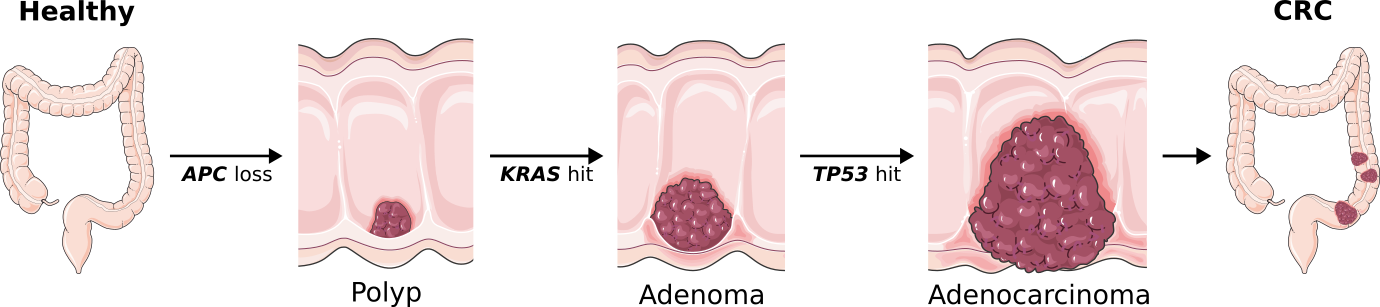
\includegraphics{01intro/figs/1BIO_CRC.png}
    \caption{something something on the canconical model of crc progression. mutations are an introduction into those used in our model. Still missing more muts that should probably be added to the figure.}
    \label{fig:1crc}
\end{figure}
% \addtocounter{figure}{-1}
\cite{van_de_wetering_-catenintcf-4_2002}
% oncogenic mutations targeting \textit{Apc}, \textit{Kras}, \textit{Braf}, \textit{Smad4}, and/or \textit{Trp53} constitute intrinsic cues that induce a crypt-progenitor phenotype in CRC cells \cite{van_de_wetering_-catenintcf-4_2002}

\subsection{The Colonic Epithelium and Colon Stem Cells}

% \colorbox{yellow}{THIS NEEDS SOME KIND OF FORESHADOWING RE LANDSCAPES and CANCER AS PLASTICITY DISEASE}

% \subsubsection{Figure on CRC hallmarks/development}
% \subsubsection{Figure on the colonic epithelia stem niche and its support and changes in CRC}
% something like \colorbox{yellow}{Armaghany et al 2012}
% \emph{This figure will be like that one on the SI vs colon from the Beumer and Clevers 2021 review, but with the right most panel being crc state. Also need to introduce the signalling driving the pro and rev csc (acc to literature) \colorbox{yellow}{Sphyris et al 2021}}

The intestinal epithelium comprises an epithelial mono-layer lining the lower gastrointestinal tract that controls nutrient uptake, coordinates metabolism, and shields against pathogens. In a homeostatic setting, intestinal epithelia has an extremely high turnover rate and is organised as distinct cell populations with absorptive or secretory functions, supported by continuously proliferating crypts \cite{bonis_intestinal_2021}. The colon and rectum form the distal end of the gastrointestinal tract and, unlike the longer small intestinal compartment, they experience a higher microbial load, lack villi, and specialise in liquid uptake \cite{kiela_physiology_2016}.

At the base of the colonic crypts reside LGR5\textsuperscript{+} \acrlong{csc}s (\acrshort{csc}s) that give rise to rapidly proliferating Transit Amplifying (TA) cells (Figure \ref{fig:1epi}A). While the specific differentiation trajectories are not yet fully understood, it seems that an Endoplasmic Reticulum (ER) stress response marks the shift from a basal proliferation state into differentiated epithelial states (Figure \ref{fig:1epi}A) \cite{heijmans_er_2013, coleman_er_2019}. Of those differentiated states the most common ones are the enterocytes with an absorptive (also called colonocytes in the colon), and secretory cells such as; mucus-secreting goblet cells, hormone-producing enteroendocrine cells, and immuno-modulatory tuft cells. 

The delicate balance of spatial and temporal control of cell fate is achieved by two opposing gradients between the basal and apical folds of the epithelium, with WNT and NOTCH signalling higher around the CSC-harbouring crypts, and BMP signalling higher towards the apical areas where absorptive cells are (Figure \ref{fig:1epi}A) \cite{bonis_intestinal_2021, beumer_cell_2021}. Continued epithelial renewal is sustained by the CSC population. Characterised by their expression of the LGR5 R-spondin receptor, CSCs are primed to receive converging signalling cues from stromal and intrinsic signals that delineate areas of cell differentiation and proliferation. 

Although this arrangement is kept relatively consistent throughout the lower gastrointestinal tract, organoid models suggest that the architecture of the homeostatic crypt in the colon appears to be, unlike that of the small intestine, more dependent on exogenous stroma-derived WNT ligands and BMP antagonists \cite{sato_long-term_2011, kondo_emerging_2019}. This difference is thought to be driven by secretory cells known as Paneth cells, which reside at the bottom of the crypts in the small intestine but are absent in the colon. Paneth cells support nearby stem cells through the secretion of antimicrobial peptides, WNT and EGF ligands, and juxtacrine NOTCH signalling. In the colon the presence of secretory cells in deeper areas of the crypts has been described \cite{sasaki_reg4_2016}, but it is believed that the niche supporting the stem compartment is mostly orchestrated by the stroma rather than by these Paneth-like Deep Crypt Secretory cells.

\begin{figure}
    \centering
    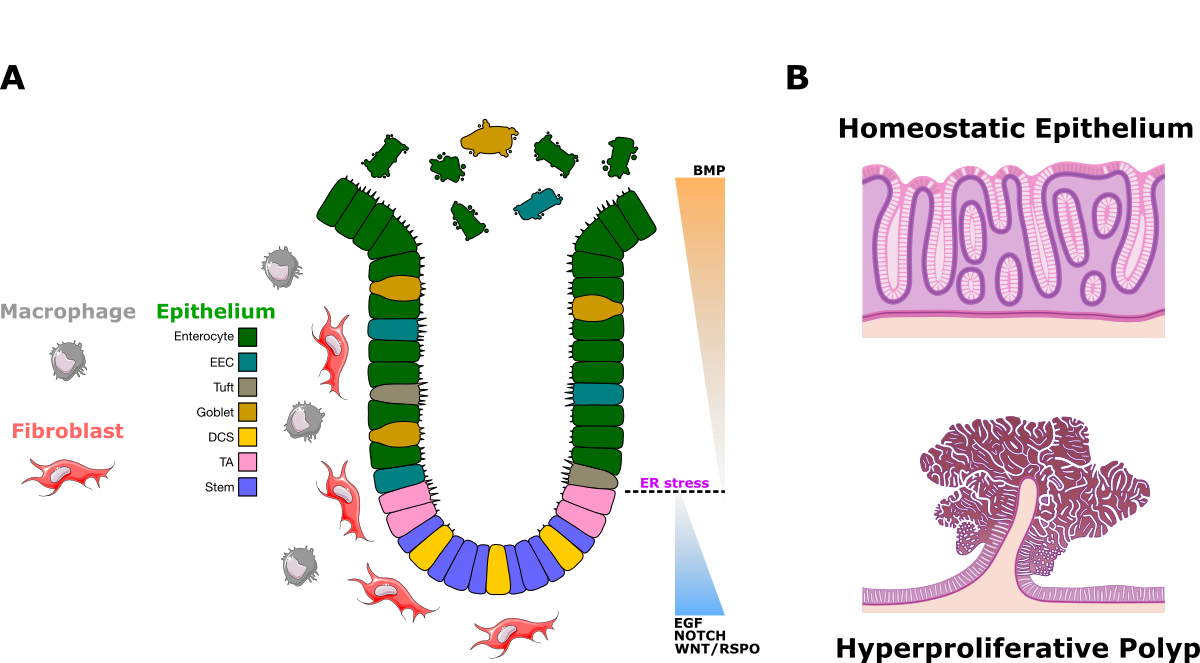
\includegraphics{01intro/figs/1BIO_gutepithelia.png}
    \caption{A) cell types and stem niches and regulation. B) Altered presentation of hyperproliferative polyps when compared to homeostatic colonic epithelium.}
    \label{fig:1epi}
\end{figure}

\subsection{Colorectal Cancer as a Heterocellular Disease}

Genetic alterations in epithelial cells commonly target niche factor signalling hubs that regulate proliferation and differentiation, enabling the CSC compartment to decouple from both pro-survival proliferative signals, and growth-inhibitory cues \cite{sphyris_subversion_2021}. This results in an emancipated and highly proliferative stem-like state (proCSC) that expands beyond the bases of the crypts and dominates the colon epithelium, thus accompanied by a general de-differentiation of the tissue (Figure \ref{fig:1epi}B).

Although it is tempting to think that the expansion of the Colonic Stem Cell (CSC) compartment in CRC is driven by this highly proliferative homogeneous proCSC state, single-cell studies have revealed the presence of additional stem cell states in both homeostatic and CRC epithelium \cite{norkin_single-cell_2020, bankaitis_reserve_2018,barriga_mex3a_2017,bues_deterministic_2022}.
Among them, revival colonic stem cells (revCSC) are emerging as a target of particular interest in cancer research. A rare population in the homeostatic intestine, revCSCs are characterised by \emph{CLU} and \emph{ANXA1} expression and exhibit a less proliferative state that, upon tissue damage, co-opts a phenotype reminiscent of foetal intestinal progenitors to replenish the injured epithelium \cite{ayyaz_single-cell_2019}. 
In the context of CRC, revCSC have been postulated as a putative drug-resistant state that can, after chemotherapy erodes the dominant proCSC state, drive relapse in some CRC patients \cite{rehman_colorectal_2021,alvarez-varela_mex3a_2022}. While the revCSC state has been associated with Hippo and YAP signalling, their exact role in relapse and the mechanisms driving the balance between revival and proliferative CSCs remain unclear.

\emph{A priori} a niche-factor independent compartment, the CRC epithelium comprised mostly of emancipated CSC and proCSC cells is still able to interact and remodel surrounding tissues. This interaction with their environment sustains the view that tumours exist not just as homogeneous clusters of malignant cells, but as a collection of malignant and non-transformed immune and stromal cells \cite{balkwill_tumor_2012}. These untransformed cells constitute the tumour microenvironment (TME), a key factor in most cancers that affect prognosis \cite{calon_stromal_2015} and therefore the subject of intense study in cancer biology and therapy development. 

In their late stage, CRC tumours consist of a complex heterocellular environment in which stromal and immune compartments have been shown to drive cancer cell progression \cite{peddareddigari_tumor_2010,isella_stromal_2015} and response to therapies \cite{tape_heterocellular_2017, toor_immune_2019}.
Cancer associated fibroblasts in particular have been linked with carcinogenesis via secretion of growth factors like EGF, HGF, VEGF and TGF-$\beta$ signalling. In addition, they have also been linked with pro-inflammatory and angiogenic roles, as well as with aiding the CRC tumour in immune evasion and invasion \cite{karagiannis_cancer-associated_2012}.
Within the immune compartment, tumour-associated macrophages are highly abundant, but their functional role within the TME is unclear. There is evidence that they both exhibit pro- and anti-tumour activity, possibly depending on their location within the adenocarcinoma and thei dominance of different macrophage sub-types \cite{martinez_m1_2014}. 
% MArginal periphery apoptosis induction via fas, M1 promoting immune response. OTH, on invasive edge TMAS help tumour, and  M2 downregulate immune response and promote angiogenesis.


\section{Organoids as \textit{in vitro} Models of Colorectal Cancer}

The complexity of CRC can be modelled and studied \emph{in vitro} using organoids, self-organising 3D cellular structures comprising stem and differentiated cells that mimic elements of \emph{in vivo} tissue \cite{huch_modeling_2015,lancaster_disease_2019,almeqdadi_gut_2019}. Mimicking the biology of the \emph{in vivo} setting, gut organoids have a basal stem niche from which differentiated states (with absorptive or secretory functions) derive from; often with an apical lumen within the organoid that accumulates dead cells \cite{sato_single_2009}.

Furthermore, heterotypic settings can be designed wherein colon epithelia organoids are co-cultured with other cell types to model stromal and immune cell-cell interactions \cite{qin_cell-type-specific_2020}. Such settings increase the complexity of organoid systems, allowing for more accurate modelling of \emph{in vivo} tissue architecture and heterotypic interactions \emph{in vitro}. 

In the context of CRC, organoids can be used to characterise both the heterogeneity of the altered colonic epithelium and its interaction with cells of the TME. Furthermore, Patient Derived Organoid (PDO) models are gaining traction as personalised avatars of human tumours \cite{su_efficacy_2023,zapatero_trellis_2023}.

\begin{figure}
    \centering
    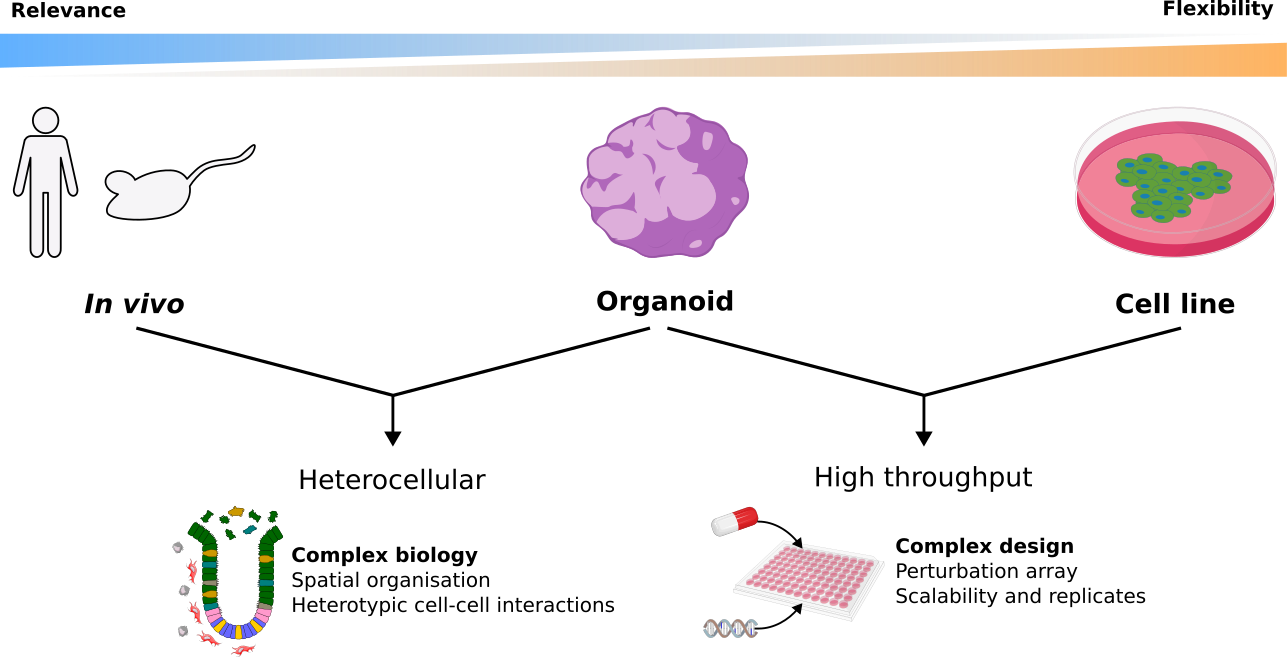
\includegraphics{01intro/figs/1BIO_organoids.png}
    \caption{organoids}
    \label{fig:1org}
\end{figure}

% \subsection{Platforms for High Throughput and Dimensional Models}

Organoids provide a balance between experimental flexibility and physiological relevance. They are complex enough to mimic the heterogeneity of \emph{in vivo} tissue while still being amenable to high-throughput applications \cite{qin_deciphering_2020}. This facilitates high throughput experimentation by allowing for the multiplexing of high numbers of experimental conditions, with for example our custom mass cytometry platform in Sufi \& Qin \textit{et al}. reaching up to 126 plex per run \cite{sufi_multiplexed_2021}.

Recent work by our lab \cite{qin_cell-type-specific_2020} has shown how both CRC genetic perturbations (\textit{shApc}, \textit{Kras\textsuperscript{G12D/+}} and \textit{Trp53\textsuperscript{R172H/–}}) and TME complexity (heterotypic epithelial organoid cultures with fibroblasts and/or macrophages) effect the biology of colonic organoids. Using a custom multivariate mass cytometry platform to analyse post-translational modification (PTM) signalling networks, Qin \textit{et al} \cite{qin_cell-type-specific_2020} found that the distribution of both cellular sub-types and states within the epithelial population changed in a similar and synergic way. They found that both oncogenic and stromal cues resulted in an enrichment of the crypt and stem niches and a reduction of cells in G0 and apoptotic states. Furthermore, their results suggest that the effects of the TME on intracellular epithelial signalling pathways might mechanistically differ from those driven by CRC mutations in the epithelial cells, even if they both share downstream signalling profiles.

This work, featuring multiple axes of variation and replicates within a single experiment, highlights the systematic scalability of organoid models. Moreover, the organoid-inherent heterogeneity coupled with heterotypic cultures justifies comprehensive single-cell analysis to be deconvoluted.
Mature bulk technologies are not poised to leverage heterogeneous 3D organoids; hence, the rapid emergence of single-cell resolution studies in recent years. Single-cell \emph{omic} approaches can deconvolute the different cell types within a heterotypic organoid system as well as resolve particular cell states within each type and even capture cellular interactions within the different compartments \cite{tape_heterocellular_2017}.


\section{Single-Cell \emph{Omic} Technologies}

During this work I leveraged two distinct single-cell technologies to characterise heterocellular organoid models of CRC; mass cytometry (MC) and single-cell RNA sequencing (scRNA-seq). They are both part of the broader family of single-cell \emph{omics} analyses, which have gained traction in characterising cellular heterogeneity at both genotypic and phenotypic levels. 

The concept of \emph{"omics"} is not well defined, but it is commonly understood to describe analyses pertaining to the study of large-scale biological datasets characterising sets of biological molecules from living entities. Some of the most common \emph{omic} studies are the fields of genomics, epigenomics, transcriptomics, and proteomics.
\emph{Omic} information can thus be used to infer cross-\emph{omic} regulatory relationships and decipher causal relations between genotype and phenotype with the right experimental settings.


\subsection{Mass Cytometry (MC)}

MC, also known as Cytometry by Time-Of-Flight (CyTOF), is a technology that merges principles of mass spectometry and flow cytometry to enable single-cell analysis of protein expression. Like flow cytometry, MC is based on tagged antibodies that bind to specific epitopes in cells, but it is able to overcome the issue of florescent spectral overlap by using monoisotopic rare-earth metals instead of fluorophores. The discrete nature of the monoisotopes compared to the broad emission spectra of fluorophores allows for the design of antibody panels that can capture up to \(1\cdot10^2\) features per cell \cite{tracey_cytof_2021}. 

Resolving total protein level information in single-cells is itself incredibly useful, but mass cytometry also excels at resolving post-translational modifications (PTMs) \cite{ochoa_functional_2019}. PTM information often determines a cell's state in relation to the cell cycle, as this process is not really regulated at the gene level but rather by a tight control of different PTM-driven checkpoints \cite{cuijpers_guiding_2018}. This capability also allows for in-depth study of intracellular signalling networks, DNA-damage responses, and apoptosis, and has already been used to characterise both cell-state and oncogene- and stroma-driven signalling changes in murine CRC organoid models \cite{qin_cell-type-specific_2020}.

Coupled with a custom multiplexing platform \cite{sufi_multiplexed_2021} \acrshort{mc} technology can analyse extremely wide experimental systems covering a large number of conditions and replicates, which proves especially useful for drug screening applications \cite{zapatero_trellis_2023}.

However, while powerful in the study of intracellular signalling, \acrlong{mc} struggles to resolve intercellular communication through the complex extracellular interactome of ligands and receptors. In contrast, \acrfull{scrnaseq} technologies can prove extremely useful for this purpose, especially when combined with intercellular cell communication databases such as CellChat \cite{jin_inference_2021} and CellPhoneDB \cite{efremova_cellphonedb_2020}.


\subsection{Single-Cell RNA Sequencing (scRNA-seq)}

With the advent of next generation sequencing (NGS) technologies, bulk-based RNA sequencing approaches were devised that could capture genome-wide transcriptomic information from a whole sample. This mature technology enabled key discoveries across a variety of fields, including tissue development and cancer biology, but its inability to resolve individual cells and their states is a key limitation in systems with complex transcriptional dynamics and multiple cell types \cite{li_bulk_2021}.
scRNA-seq overcame this issue by capturing transcriptomic information at the level of individual cells. Now, a collection of discrete transcriptomic profiles can be pieced together to recapitulate continuous differentiation trajectories, or complex heterocellular systems could now be resolved into their individual cell types \cite{haber_single-cell_2017}. However, while powerful, scRNA-seq comes with significant technical challenges and costs. 

Mature and highly optimised microfluidic droplet-based approaches tend dominate the commercial market, with 10X Genomics offering commercial products \cite{kitzman_haplotypes_2016} that perform the best in terms of UMI and gene / cell detection whilst being a high-throughput application \cite{ding_systematic_2020}.

\begin{figure}
    \centering
    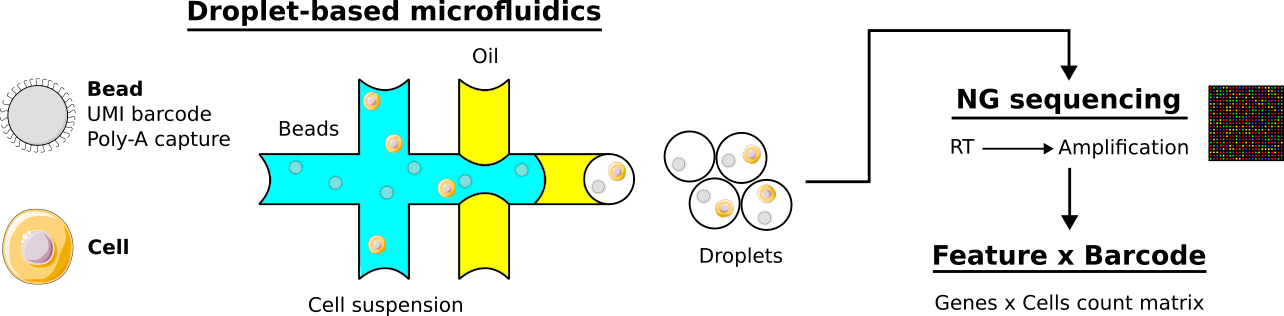
\includegraphics{01intro/figs/1TECH_scRNAseq.png}
    \caption{cell types and stem niches and regulation. NG, next generation (sequencing).RT, reverse transcription. UMI, unique molecular identifier.}
    \label{fig:1tech}
\end{figure}

Droplet-based scRNA-seq methods work by encapsulating individual cells and uniquely tagged beads into water-in-oil droplets, where the cells and beads constitute the dispersed phase and the oil forms the continuous phase encapsulating the droplets \cite{macosko_highly_2015} (Figure \ref{fig:1tech}). During amplification using the poly-A tail capture primers (Figure \ref{fig:1tech}), a unique cellular barcode is added and shared across all products from a single droplet, and a unique molecular identifier (UMI) is also added as a transcript-specific tag before amplification.
Resolving the single-cell level data then relies on only one cell being present in each droplet, so to avoid duplicates a significant percentage of droplets are left empty \cite{abate_beating_2009}. scRNA-seq methods are also characterised by dropout effects, as they capture genes with relatively low yields, resulting in sparse and noisy datasets \cite{qiu_embracing_2020}. 

Despite their good performance and field dominance, high throughput droplet-based microfluidic scRNA-seq approaches still represent a significant monetary burden due to library preparation, which negatively affects scalability and might even, in extreme cases, jeopardise scientific validity by potentially constraining the presence or number of replicates \cite{zimmerman_practical_2021}.
    % \colorbox{yellow}{A practical solution to pseudoreplication bias in single-cell studies} (https://www.nature.com/articles/s41467-021-21038-1) talks about issues derived from the fact that often times not replicates available and that individual cells from the same sample ARE NOT replciates, whereas in DE they are common treated as completely distinct obeservations when comparing clusters.

To overcome this burden, there has been an emergence of microfluidic-free approaches in recent times. Clark \textit{et al.} recently developed PIP-seq \cite{clark_microfluidics-free_2023}, a droplet-based approach based on vortexer emulsification that aims to reduce costs and protocol complexity. By contrast, split-pool barcoding approaches do require a considerable amount of liquid handling steps but promise incredible scalability by using combinatorial split and pooling steps to uniquely barcode at once all cells within a sample \cite{rosenberg_single-cell_2018}.

In the context of CRC, scRNA-seq has been widely used to describe intestinal epithelia \emph{in situ} \cite{haber_single-cell_2017} and even in organoid models, but to date no systematic analysis of colon epithelia across multiple perturbation axes capturing both CRC oncogenic status and changes in the TME has been performed. 

Also known as massively parallel methods, NGS transcriptomics requires the isolation and lysis of cells, reverse transcription of their RNA into cDNA, and then amplification to generate sequencing libraries (Figure \ref{fig:1tech}). Despite being relatively mature technologies, it is still an advancing field, with costs reduction following Moore's Law during the last decade \cite{wetterstrand_dna_2022}.
Emerging third-generation sequencing technologies \cite{check_hayden_genome_2009} are capable of sequencing at the single-molecule level and generally produce reads that are longer than those of NGS approaches \cite{eid_real-time_2009,deamer_three_2016}. Able to also measure multiple \emph{omic} layers \cite{ni_deepsignal_2019}, they are poised to challenge the more common NGS technologies in the future.


\section{Single-Cell \emph{Omic} Data Analysis}

Single-cell technologies generate \emph{omic} scale profiles at the resolution of individual cells, so that complex heterocellular systems like organoids or \textit{in vivo} tissues can be profiled.
However, these approaches produce extremely high dimensional datasets due to the large-scale nature of \emph{omic} data and the single-cell resolution of the technology. Although the large amount of data generated certainly does present a technical challenge, it also allows for a myriad of complex analytical approaches that leverage its complexity and depth to the fullest extent \cite{mincarelli_defining_2018,qin_deciphering_2020}. 

\subsection{The Three Axes of Dimensionality}

% \subsubsection{FIG on data characteristics and general workflow. Also types of analyses for scRNA-seq in specific}
% Big one, review style.
% Convey the info presented in both FIgures 2 and 5 of Xiao's review. Most important from here is the broad pipeline of analysis.
\begin{figure}
    \centering
    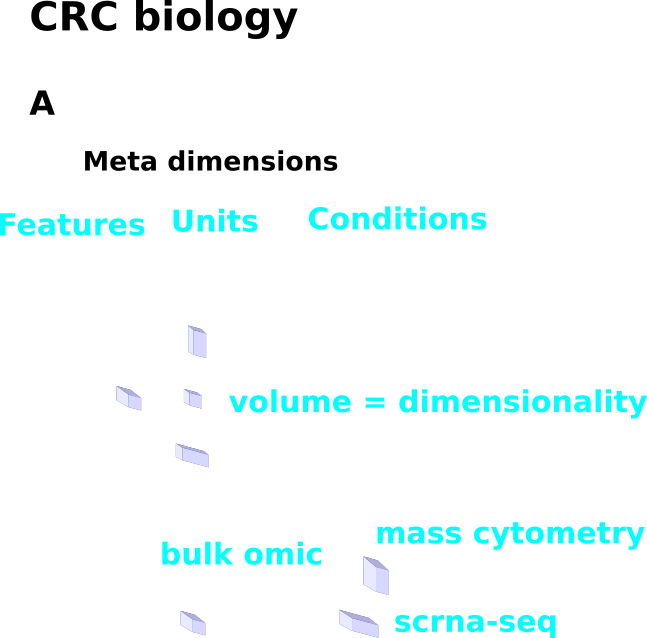
\includegraphics{01intro/figs/1COMP_dims.png}
    \caption{}
    \label{fig:1dims}
\end{figure}


Within the context of \emph{omic} approaches, data dimensionality can be thought of three distinct axes; 1) the number of features to be measured, such as genes or proteins, 2) the number of units whose features are measured, and 3) the number of conditions, groups of units representing a particular biological setting \cite{qin_deciphering_2020}. Thus, a concept of meta-dimensionality is useful to refer to all axes at once.
The unit of measurement is dependent on the methodology used, with bulk methods measuring at the level of whole samples whereas single-cell approaches resolve individual cells. Some spatial \emph{omic} methods fall somewhere in between bulk and single-cell approaches, examining specific regions of a sample containing a small number of cells \cite{vickovic_high-definition_2019,marx_method_2021, williams_introduction_2022}.

Thus, single-cell approaches can generate extremely high-dimensional datasets due to the large-scale nature of \emph{omic} data and the single-cell resolution of the technology. This presents new data analysis challenges that are further compounded when applied to highly scalable models such as organoids that allow for high numbers of conditions to be measured. Machine learning approaches and dimensionality reduction techniques are thus commonly applied to extract meaningful information from high dimensional single-cell data, and, while there is still no uncontested consensus, the more common approaches will be discussed below.
% This has come with added difficulties such as resolving individual cells from complex 3D organoid structures and dealing with the high dimensionality of the resulting data14. 


\subsection{Data Integration}

The essence of data integration is the merging of multiple discrete datasets, and their applications range from batch correction to disjoint cross-modality integration, where modality refers to different sets of measures generally across different \emph{omic} fields.

Of the different types of integration tasks, the most common is between datasets with feature overlap but different units (cells) being measured. This type of integration is needed when datasets are acquired as different events, where generating a combined feature space onto which the cells are projected is relatively straightforward (if indeed necessary at all) and the goal is to remove any technical noise while conserving the biological signal. Data integration approaches range from simple linear methods like mean-centring adjustment commonly used for batch effect correction \cite{hornung_combining_2016}, to more complex approaches such as canonical correlation analysis \cite{butler_integrating_2018} which uses shared anchors to integrate datasets with partially overlapping features. With the later having a tendency towards over-smoothing biological signals, recent methods like STACAS \cite{andreatta_stacas_2021} have been proposed to integrate samples with heterogeneous cell states that might only partially overlap.

Alternatively, sometimes it is necessary to integrate across datasets joint along the cell axis but with different feature sets. A quite common occurrence when dealing with multi-modal techniques, this task can be approached in several ways. The oldest approaches attempted to map the modalities into a shared feature space using cross-omic prior knowledge \cite{chen_assessment_2019}, but these have mostly been replaced by techniques that consider the different modalities to be representations of the same underlying manifold, thus attempting to align the two spaces with techniques such as optimal transport while also optionally incorporating prior knowledge \cite{cao_unsupervised_2020, cao_multi-omics_2022}.

Finally, the most challenging integration tasks are those where there is no overlap between feature or unit spaces. In these cases, integration relies on the assumption that the cells analysed belong to the same underlying manifold of cell states (i.e. they are different snapshots of the same biological process being sampled), and allows for \emph{in silico} generation of cross-omic integrated space from multiple disjoint unimodal datasets and atlases \cite{amodio_magan:_2018,lotfollahi_mapping_2022,cao_multi-omics_2022}.


\subsection{Common Practices for Data Analysis}

% \subsubsection{FIG on data characteristics and general workflow. Also types of analyses for scrnaseq in specific}
% Big one, review style.
% Convey the info presented in both FIgures 2 and 5 of Xiao's review. Most important from here is the broad pipeline of analysis.

% \cite{luecken_current_2019} Classical scrnaseq

% \cite{slovin_single-cell_2021}(https://link.springer.com/protocol/10.1007/978-1-0716-1307-8_19) Review/protocol on the different comp steps of analysis. Idea of nothing being standard

% \cite{heumos_best_2023} Heumos et al 2023: Best practices for single-cell analysis across modalities. MOst recent, from the multiomics angle

\begin{figure}
    \centering
    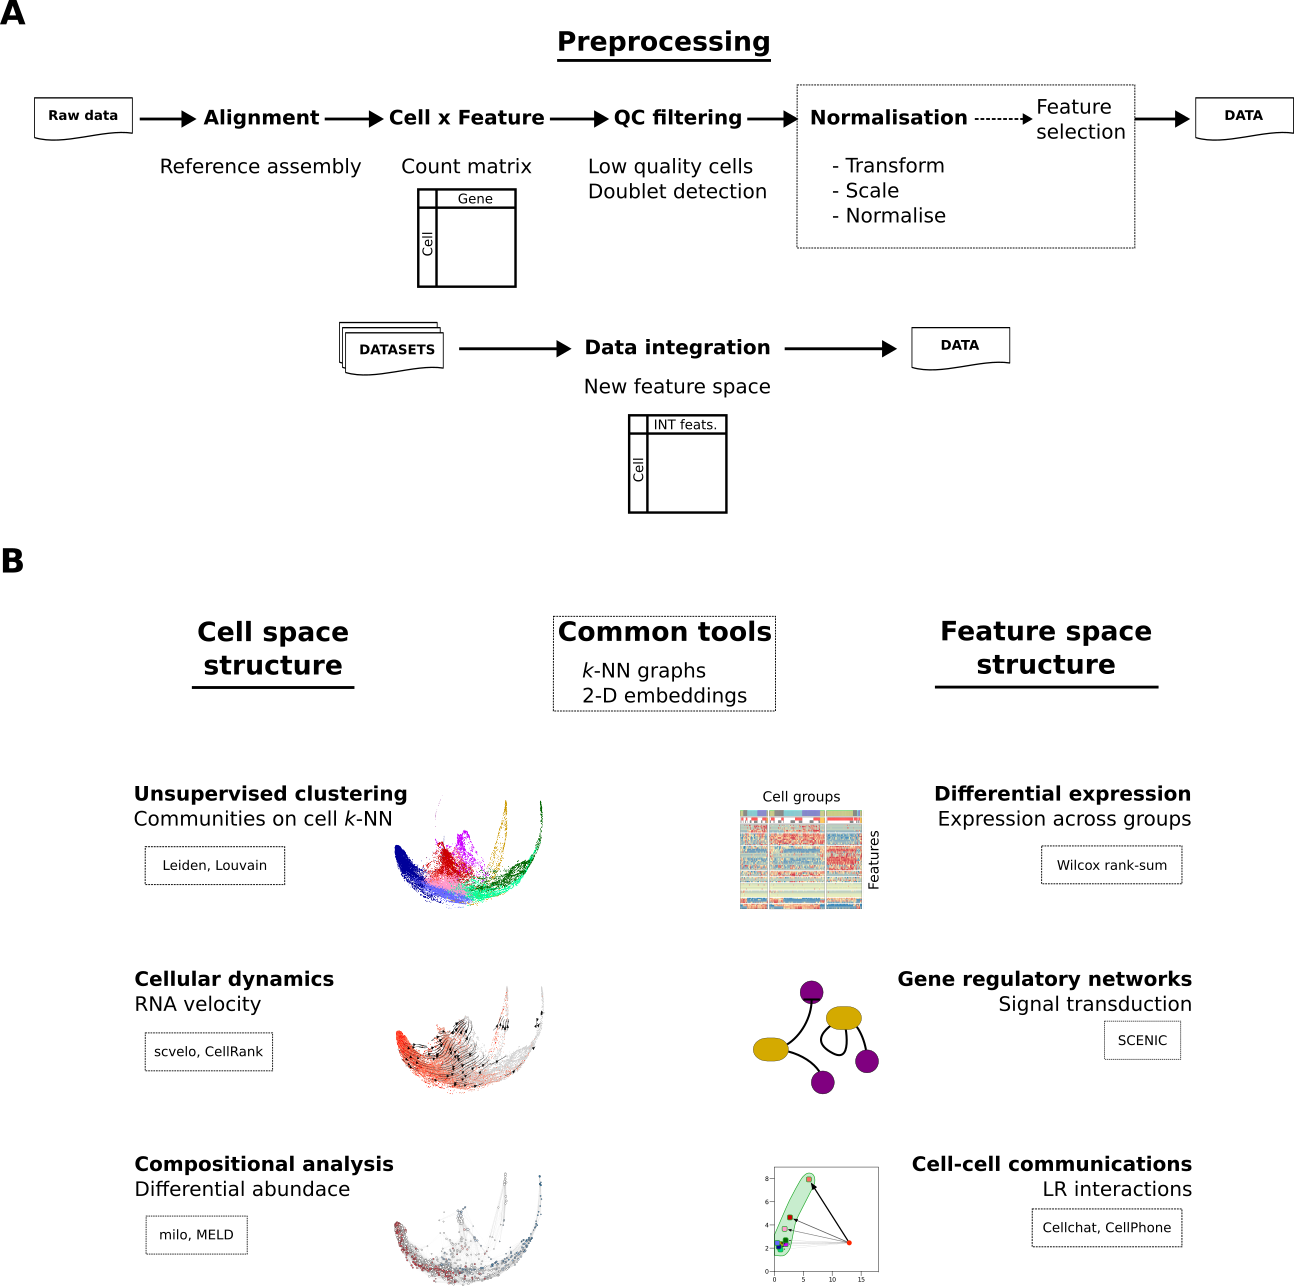
\includegraphics{01intro/figs/1COMP_analysis.png}
    \caption{}
    \label{fig:1pipe}
\end{figure}

Analysis of single-cell omic data is a growing and mostly non-standardised field where a myriad of tools and approaches have been proposed to leverage rich and high-dimensional single-cell omic datasets. Structurally, it is commonly divided between pre-processing and downstream analyses, and while there are some general guidelines and approaches pervasive to the field \cite{luecken_current_2019, heumos_best_2023}, even very established tenets like the unsupervised clustering of cells continue to be debated.

\textbf{Pre-processing} of the data encompasses from more upstream tasks such as sequence alignment and feature normalisation, to further downstream steps like data integration (Figure \ref{fig:1pipe}A), commonly done after a certain degree of exploration of the feature and unit spaces. In the case of scRNA-seq, the first step is to align the sequenced reads against a transcriptome of reference \cite{dobin_star_2013,bray_near-optimal_2016}. This process enables the generation of a count matrix that represents the unit X feature space, i.e. the gene expression detected for each gene (feature) on each cell (unit).

Once the cell X feature matrix has been generated, filtering-based quality control (QC) is performed, whereby cells that do not meet thresholds set on the feature space are removed. Commonly, as part of QC protocols doublet and apoptotic or otherwise compromised cells also get removed.
The filtered data is then transformed and scaled to account for factors that might obscure biological signals, such as differences in cell metrics or feature detection capabilities and sequencing depth. These normalisation steps vary according to the data being analysed, so that for mass cytometry datasets intensities are usually normalised used an inverse hyperbolic sine transform (\(asinh x\)) with a co-factor of \(5\) \cite{bendall_single-cell_2011,guldberg_computational_2023}. For scRNA-seq the approaches range from simpler (and seemingly more robust) log-based transformation \cite{ahlmann-eltze_comparison_2023} and depth-based normalisation \cite{booeshaghi_depth_2022}, to more complex methods like SCTransform \cite{hafemeister_normalization_2019} that use Generalised Linear Methods with Pearson residuals and are able to regress out unwanted sources of variation.

Feature selection is a common pre-processing step that precedes downstream analysis. In the sequencing field, feature selection is commonly limited to selecting highly variable genes, as it is assumed that those will carry relevant biological information and will also speed up compute time by limiting the large feature space. In less feature-rich \emph{omic} technologies, such as mass cytometry, the aim of feature selection is rather a temporary process wherein certain features are used to determine a specific metric (such as nested Boolean gating of cell-cycle associated PTMs to determine cell state \cite{behbehani_single-cell_2012,qin_cell-type-specific_2020}). Often times it is done in conjunction with the normalisation steps commonly performed upstream (Figure \ref{fig:1pipe}A).

If relevant, data integration is commonly performed after the QC and normalisation steps, most commonly with the aim of either removing batch effects between samples or to generate a shared feature space across modalities \cite{cao_multi-omics_2022}. 

Dimensionality reduction (DR) techniques aim to reduce the complexity of the the data while still preserving as much information as possible. If we consider that individual cells belong to a manifold where local structure can be mapped to an Euclidean space our aim would be to preserve distances between cells both in this local space but also at the global level across distant points in the manifold. Principal Component Analysis (PCA) \cite{pearson_liii_1901,jolliffe_principal_2016} was defined in the pre-computational era of the early 20\textsuperscript{th} century and is still commonly used due to it's simplicity and speed. However, PCA is only capable of capturing linear relationships, and thus is generally used as an intermediate DR approach where high dimensional data is compressed to a feature space of \(1\cdot10^1\) to \(1\cdot10^2\). Later DR approaches aim to capture non-linear relationships and to better reflect the underlying manifold, and include methods like Diffusion Maps \cite{coifman_diffusion_2006}, t-SNE \cite{van_der_maaten_visualizing_2008} and UMAP \cite{mcinnes_umap_2020}. While these methods are able to preserve local distances from the manifold in the embedded space, in recent years there has been a push towards consistently preserving global manifold structure too. Methods like PHATE \cite{moon_visualizing_2019} and its multi-scale derivative \cite{kuchroo_multiscale_2020} represent some of those efforts that have been developed specifically for the field of single-cell \emph{omic} data.

\textbf{Downstream analyses} vary in both aims and methods used, so much so that there is no uncontested gold standard data analysis workflow \cite{slovin_single-cell_2021}. Despite this, all approaches tend to share a common purpose in finding structure in both the feature space (i.e. genes in scRNA-seq) and in the cell space (Figure \ref{fig:1pipe}B).

Determining structure in the unit (cell) space generally translates to identifying a cell's state or type. This is commonly accomplished via unsupervised clustering methods that groups cells based on their location within a \emph{k}-Nearest Neighbours (\emph{k}-NN) graph that captures their transcriptional similarities. The output of these community detection algorithms \cite{blondel_fast_2008,traag_louvain_2019} is indeed unsupervised, but clusters are most commonly presented as annotated entities (sometimes via merging/splitting of unsupervised clusters) through manual approaches that require prior biological knowledge and curation based on known cell markers, or through reference mapping and label transfer from annotated atlases \cite{lotfollahi_mapping_2022}. Clusters are thus discrete groups of cells (be it types or states), so to attempt and reconstruct the structure of the continuous biological process being studied, trajectory inference methods such as Slingshot \cite{street_slingshot_2018} and PAGA \cite{wolf_paga_2019} have been developed. These trajectories are mapped onto an inferred pseudo-time axis, and this process can be further complemented by RNA velocity. RNA velocity \cite{la_manno_rna_2018} is a method that refers to the usage of splicing kinetics to model transcriptional dynamics and infer vectors of tanscriptional change (i.e. the direction and rate of gene expression change) along the manifold of cells. These vectors can either be used on their own to infer a pseudo-time axis \cite{bergen_generalizing_2020}, or act as an input layer for further downstream analyses that attempt to determine cell fates (as opposed to/in addition to cell states/types) \cite{lange_cellrank_2022}.

Compositional analysis refers to the methods used to explain how structure in the cell space is affected by perturbations across different conditions. The first single-cell \emph{omic} studies presented relatively simple experimental designs (due to high costs and low throughput) and thus their work tended towards the description of a particular condition. However, as technologies have advanced and costs have trended downward, more complex experimental designs have emerged where it is pivotal to model and quantify the effects of perturbations (e.g. mutations and drug treatments in the context of CRC). Hence the emergence of compositional analysis methods in recent times, such as Differential Abundance \cite{lun_testing_2017,dann_differential_2022}, MELD \cite{burkhardt_quantifying_2021}, and Trajectory Net \cite{tong_trajectorynet_2020}. Furthermore, there are also a set of approaches to \emph{in silico} model perturbations that were not part of the experimental design \cite{lotfollahi_scgen_2019,yuan_cellbox_2021,lotfollahi_learning_2021}, but these methods tend to struggle when modelling genes with low expression values.

While trajectory analysis and RNA velocity are extremely useful for determining cellular dynamics in a differentiation setting, a cell-based metric of pluripotency is also of special interest to discern stem cells from differentiated cell fates. To this end the concept of Signalling Entropy Rate was postulated \cite{teschendorff_signalling_2014}, which argues that the higher the entropy of a cell's transcriptomic profile, the less differentiated and thus higher pluripotency degree it presents. Currently there are several methods to estimate cell pluripotency from scRNA-seq data, most relying on Signalling Entropy Rate and computationally faster approximations like the degree of correlation between the transcriptome and Protein-Protein interaction matrices \cite{teschendorff_single-cell_2017,gulati_single-cell_2020,senra_origins_2022}. 

Exploring the structure within the feature space is key towards understanding the biology at a mechanistic (and not just descriptive) level. In the context of scRNA-seq, structure in the feature space is commonly determined through Differential Expression (DE), which determines the degree and statistical significance of changes in a gene's expression across individual cells or groups of them (e.g conditions, labelled cell identities or cellular neighbourhoods). The most common DE methods are pseudo-bulk approaches derived from the mature field of bulk sequencing \cite{robinson_edger_2010,finak_mast_2015} or population comparison tests like the Wilcoxon signed-rank test. These methods are commonly applied to compare clusters, in which case they generate a list of markers characteristic of each cluster/population, but might also be used to compare conditions or even cellular neighbourhoods \cite{missarova_sensitive_2023}. The resulting gene markers can then be passed through Gene Ontology \cite{ashburner_gene_2000} and pathway databases \cite{kanehisa_kegg_2017,turei_integrated_2021,gillespie_reactome_2022}, or Gene Set Enrichment Analysis tools \cite{subramanian_gene_2005} to identify putative biological processes for each cell group. 

Much like in the context of cell structure, \emph{k}-NN graphs of genes can also be constructed from either interaction databases or gene expression data. These graphs can then be used to determine gene modules and gene regulatory networks \cite{aibar_scenic_2017}, and represent a relatively unexplored avenue for emerging methods when compared to the much more common cell-graphs.
Cell-to-cell communication tools also leverage these interaction databases with the aim of inferring cellular interactions through the co-expression of ligands, receptors, and other interaction member genes \cite{armingol_deciphering_2020}. Methods like CellPhoneDB \cite{efremova_cellphonedb_2020} and CellChat \cite{jin_inference_2021} predict ligand-receptor interactions by identifying clusters of cells that express receiving or sending members of the interactions, and can be used together with spatial studies to refine their predictions \cite{hu_cytotalk_2021,kanemaru_spatially_2023}. Given the broad diversity in methods for determining an interaction and the different interaction databases used, ensemble methods such as LIANA have been designed to aggregate often conflicting cell-cell communication results \cite{dimitrov_comparison_2022, baghdassarian_combining_2023}. 


\subsection{Limitations and New Avenues}

Accessibility and scalability advancements to single-cell multiomic technologies are empowering a complex and multifactorial view of cell identity. This is especially relevant in the field of cancer research, where views are shifting from the canonical genotype-driven cancer cell state, toward plasticity-driven phenotypes. 

However, this nuanced view of cell identity clashes with the concept of cluster derived cell types, especially those derived from transcriptomic data that could be argued are better suited to capture a cell's state. Furthermore, our understanding of biological processes wherein cells represent individual points along a continuum is not really suited to discrete cluster-based groups. In response to this necessity, there has been a series of emerging cluster-free approaches, such as the concept of cellular neighbourhoods as applied by John Marioni's lab, or the notion of cellular archetypes and metacells. The cellular neighbourhood approach was first implemented as miloDA in the context of compositional analysis \cite{dann_differential_2022}, and has recently been adapted for DE tasks \cite{missarova_sensitive_2023}. They iterate on the concept of clusters defined on a \textit{k}-NN graph to that of cellular neighbourhoods; which both contain fewer cells than a typical cluster and can overlap over the same regions of the graph. Cellular archetypes and metacells represent a more orthogonal way of tackling the limitations of cells clusters, as rather than aiming to capture discrete cell types they aim to capture cell states \cite{baran_metacell_2019, wang_non-linear_2022}. Thus, within each metacell state, all cells should ideally represent the same biological state defined by a unique profile of gene regulatory programmes and only be distinguished by technical noise. With new methods developed to address multiomic data and cross-patient integration \cite{persad_seacells_2023}, metacell-based approaches appear perhaps poised to replace the ubiquitous unsupervised clustering approaches.  
This view of cells as landmarks on a continuous landscape is far from a novel concept. In the mid 20\textsuperscript{th} century, Conrad H. Waddington illustrated the process of an epigenetic landscape where pluripotent cells would roll down into valleys of terminally differentiated states \cite{ch_waddington_waddington_1957}. However, his effort and subsequent ones since then have mostly been of a rather subjective and artistic nature. Reconstructing such landscapes from biological data is not an untenable task anymore, as omic profiles from single-cells can be embedded together and mapped onto a 2D space. Sculpted by cellular pluripotency metrics, such landscapes have already been proposed, but used embedding spaces that do not accurately reconstruct a continuous space that captures global structure and did not leverage information on transcriptional dynamics \cite{chen_single-cell_2019}. 

The idea of cell-cell graphs derived from gene or protein data is also central and common to virtually all single-cell omic analyses, including scRNA-seq and mass cytometry. \emph{k}-NN graphs of feature nodes however are a less exploited niche, often relegated to the study of gene regulatory networks and systems biology approaches. However constructing such graphs is not a trivial task, for coexpression metrics generally do not capture gene-gene interactions, most gene regulatory networks do not account for directionality \cite{chen_inferring_2019}, and curated interaction databases \cite{turei_integrated_2021} are not consistently analysed in a directed way. Hence I explore a novel approach of assembling directed gene-gene \acrfull{kg}s and then projecting cells into the graph based on their transcriptional profile, thus treating the cells as signals on a gene graph. Similar methods with comparable goals are emerging \cite{lefebvre_large-scale_2021}, suggesting a neeed for further method development in this field.
% Inherently a modality agnostic approach, it can be coupled with emerging multimodal approaches that can capture at once intra and intercellular communication features, like phospho-seq \cite{blair_phospho-seq_2023} [or Jamie's signal-seq]. -> perfect tool to solve inter- and intra-cell communications at the single-cell level without relying on clusters and in a modality agnostic way. 

% \colorbox{yellow}{Too specific, this should rather perhaps go into the intro for chapter 06}

    % Biological models already there, modelling communications between and within cells in a directed manner like pybravo\cite{lefebvre_large-scale_2021}. Gene-gene graphs can thus be used for cell-cell communicatoin analysese like scTenifoldXct \cite{yang_sctenifoldxct_2023} or leveraging sptial info too like in Fischer \& Schaar et al. \cite{fischer_modeling_2022} and even to de novo generate signal transduction networks from scRNAseq data like in Cytotalk \cite{hu_cytotalk_2021}.
    
    % Possible thanks to development of KG embedding methods and signal processing approaches able to deal with heterogenous directed hierarchical graphs. 
    % Empowered by emerging multimodla approaches that can capture at once intra and intercellular communication features, like phospho-seq \cite{blair_phospho-seq_2023} or Jamie's signal-seq. 
    
    % Gene embedding methods are growing , so are graph signal processing approaches. 
    % Discuss the embedding methods of these graphs:
    % Complexity in terms of structure, directionality and type of interaction. All of this is very important, unlike in undirected knn grpahs ubiquitous to omic analyses.
    % This means that we need some methods able to compute all of this complex relations in multi relation directed graphs  (MultiDiGraph). methods have been developed, transE \cite{bordes_translating_2013}family, graph convolutional networks, and the stuff from he stanford dawn group on  hyperbolic embeddings  \cite{chami_hyperbolic_2019} and general ML approaches applied to non euclidean spaces.
    % non euclidean space like hyperbolic spaces are keys because graphs with important hierarchical structure [as is biological signalling] is much better capture in a hyperbole than in a plane \cite{bronstein_geometric_2017,nickel_poincare_2017,chamberlain_neural_2017}.[the first one is general Euclidean =bad, the later ones refer to the cocnept of hierarchical graph better on hyperboles than planes].


\section{Hypothesis and Aims}


Organoids represent a robust model able to recapitulate \acrshort{crc} dynamics and its interaction with the \acrshort{tme}. The high dimensional information captured by single-cell \emph{omic} approaches and the diverse field of analyses promise the potential of untangling and describing even the most complex of biological processes. 
In light of this, \textbf{I hypothesise that colon-epithelia polarisation by endogenous and exogenous cues can be described using single-cell analyses of the organoids}.

First I present my efforts identifying and solving gaps in the method space that can facilitate \acrlong{mc} analyses broadly. In Chapter \ref{03cytof} I introduce CyGNAL, a workflow that aims to facilitate standard \acrshort{mc} data analysis steps for a non-computational audience. Additionally I also discuss and showcase the use of machine learning approaches to automate cell state classification for \acrshort{mc} data.

To test the main hypothesis I aim to perform a comprehensive and state-of-the-art single-cell analysis of CRC organoids to: 1) systematically describe the colon epithelial stem regulation, and 2) \emph{in silico} infer mechanisms of regulation that have been subsequently tested \emph{in vitro} by colleagues \cite{cardoso_rodriguez_single-cell_2023}. 
Chapter \ref{04seq} presents the main corpus of results from this analysis.
In Chapter \ref{05vr} I present a novel method to generate data-driven Waddington-like landscapes that capture the underlying continuous processes of transition and differentiation, and I demonstrate how they can be used to model the landscape of colon epithelial stem regulation.

Finally in Chapter \ref{06kg}, I further my aim towards solving a lack of methods for both intra- and inter-cellular communication analyses by exploring a \acrshort{kg}-based approach to study cell communication in organoid-fibroblasts co-cultures. Appendix \ref{appendix:pykrack} presents \emph{pyKrack} a standalone tool and package for computing hierarchy scores on directed graphs, such as a cell-communication interaction graphs.


\chapter{Materials and Methods}
\label{02methods}

\section{CyGNAL}

Previous to analysing the data in CyGNAL, mass cytometry datasets are debarcoded as needed (using the tool in https://github.com/zunderlab/single-cell-debarcoder) and initial data pre-processing and quality control is carried in Cytobank (https://www.cytobank.org/) (see the leftmost section of Figure 1). In that platform, the single cells are gated for Gaussian parameters, their DNA content, and uptake of cisplatin using manual gates. Gating on cell state and cell type specific markers can also be done in order to both eliminate doublets but also to identify cells belonging to each state or type; information which can then be used to train the cell state classifier among others.

Written mainly in Python and R, CyGNAL (CyTOF SiGNalling AnaLysis) is a pipeline constituted as 5 main steps. These are divided into pre-processing (initial step, always run independently of the analysis to be performed), scoring as two steps using  Earth Mover’s Distance (EMD, also known as the Wasserstein metric)22 and Density Resampled Estimate of Mutual Information (DREMI)23,24, visualising the scores as either heatmaps or Principal Component Analysis (PCA) plots, and embedding the cells themselves in a two-dimensional UMAP (Uniform Manifold Approximation and Projection) space25. It is important to note that for calculating the EMD and DREMI scores and computing the UMAP space, the data is first normalised within their respective steps using a hyperbolic arcsine transformation with a cofactor of 5, as is standard in the mass cytometry field.

During the pre-processing step CyGNAL loads in mass cytometry files either in plain text format or in the Flow Cytometry Standard format (FCS)26. Intercompatibility between both formats is ensured using the Python packages fcsparser27 and fcswrite28, and the R package flowCore29. In addition to ensuring format consistency and allowing for datasets to be saved in either format, during the pre-processing step channel names are parsed to a) eliminate empty channels, b) clean up double spaces and underscores, and c) ensure each cell has a unique ID encoded in a new column called “Cell\_Index”. Finally, it is also here where a panel\_markers.csv file is generated containing all columns present in the dataset that were identified as markers. This file can then be used downstream to select which markers are to be used in the scoring and UMAP steps.

CyGNAL’s UMAP calculation uses the umap-learn package for Python (https://github.com/lmcinnes/umap)25 to assign each of the cells in the dataset a pair of coordinates on a UMAP space. This space is computed using the set of markers defined by the user in the panel\_markers.csv file and can be calculated on either just one processed dataset or a series of datasets as long as they have shared markers in their panel. The resulting coordinates are appended as a new pair of columns to the original datasets, facilitating visualisation of this space elsewhere by the user.


Both the EMD and DREMI scores are computed using the Python package scprep30 and have their respective steps in CyGNAL that take in multiple processed datasets (with each representing e.g. conditions or populations). In the EMD calculation, a series of scores is given to the markers (chosen with the panel\_markers.csv) based on how a particular marker is distributed in a variable dataset when compared against a reference (either the sum of all datasets imputed or a particular control selected by the user). On the other hand, the DREMI calculation is performed independently in a per dataset basis, as each of the datasets will get its own set of scores representing each of the possible combinations of markers in the panel. In DREMI the scores reflect how linked marker A is to marker B using a derivate of the mutual information between the two. In the context of PTM network signalling analysis, EMD is used to quantify PTM node intensity and DREMI to score PTM-PTM edge connectivity; both measures can then be used to build signalling networks as those shown in Qin et al. 2020. The outputs of both scoring systems are saved as plain text files that can be plotted using CyGNAL’s visualisation steps below.

Finally, once the user has computed either score, the last step in the pipeline allows for an interactive visualisation leveraging R’s Shiny apps31 using two Python scripts that call in the R scripts in the background needed to host the ShinyApp. The first of those scripts generates a series of heatmaps using the ggplot32 and ComplexHeatmap33 packages. These heatmaps show the relevant scores; with the names of the datasets used in the calculation step as columns in the horizontal axis and the names of the markers in the vertical axis as rows. Colour ranges, columns, and rows shown can all be tweaked by the user through the graphical interface. The second of the scripts computes a PCA on the scores using the FactoMineR package34, treating each of the datasets used in the calculation as observations and the scores for the markers (or marker combinations in the case of DREMI) as variables. In all cases all plots generated can be saved as images for later use, and within the PCA ShinyApp the computed PCA coordinates can also be downloaded to facilitate custom generation of plots elsewhere.


\section{scRNA-seq Data Analysis}

Instead of self plagiarising, go to the now deleted earlier drafts where the methods were explained in greater detail. Then rewrite the text instead of copy/pasting

\subsection*{Wet Lab Data Generation}

This work wasn't carried out by me and this should be made very clear. Instead of detailing it here, perhaps it would be best to reference the preprint/article once up?

\subsection*{Sequencing}

While this is technically wet lab and I didn't carry it out, it is important to detail the characteristics of the library and sequencing used.

% scRNA-seq libraries were generated with the 10X Genomics Chromium Next GEM Single Cell 3' Reagent Kits v3.1 (Dual Index) and sequenced with the Illumina NovaSeq 6000 System (2$\times$ 150 bp paired-end reads), aiming at 60,000 read pairs per cell and 2,000 cells per cell-type per sample.

\subsection*{Data Processing}
Raw->fastq->align->count matrix
% Raw scRNA-seq data was converted to FASTQ files and processed with the 10X Genomics Cell Ranger pipeline version 5.0.1. Sequencing reads were aligned to a custom GRCm38 reference genome containing the sequences of \hl{\textit{DsRed} and \textit{eGFP}} transgenes present in fibroblasts and organoids respectively.

QC
% The resulting gene count matrices were analysed with the R package \textit{Seurat} version 4.0.4[\hl{ADD REF}]. The analysis pipeline encompasses quality control, data normalisation, data integration, dimensionality reduction, cell clustering, and analysis of differential gene expression. Genes found in less than 4 cells were removed during QC and only cells with at least 600 unique genes identified were kept for downstream analysis. The total number of detected sequences typically ranged from 1,200 to 80,000 per cell, and the actual values were manually determined based on dataset sequencing depth and cell-type composition. For the integrated epithelial object in Figure 2, an additional filtering step was performed to remove cells with undetectable expression for any one of the bona fide pan-epithelial genes \textit{Epcam}, \textit{Krt8}, \textit{Krt18}, \textit{Krt19}, \textit{Cldn7}. Cell-cycle regression was performed using the \textit{sctransform} function. 
% % Log-normalised gene expression values were used for the downstream analyses.

\subsection*{Integration}
Integration
% Dataset integration was performed using Seurat's reciprocal PCA (RPCA) implementation \cite{hao_integrated_2021} (k.anchor=12) as it has been optimised to handle large datasets. The integrated object presented Figure \ref{fig:fig1}B was computed using all cells from the 20 conditions shown in Figure \ref{fig:fig1}A, resulting in a total of 58,726 cells with the integrated assay limited to 2,000 genes. The integrated object presented in Figure \ref{fig:fig2}A was computed using just the epithelial cells from all conditions, resulting in an object with 29,452 cells limited to 4,000 genes.

\subsection*{Dimensionality Reduction}
seq->emd->pca and normal DR
% To generate the EMD PCA plots shown in Figure \ref{fig:fig1}C,  log-normalised gene expression data (the RNA assay) of all cells of a particular cell-type (epithelial cells, fibroblasts, or macrophages) were exported from the integrated object. EMD scores for the top 6,000 variable genes of each condition were calculated with CyGNAL \cite{cardoso_tape-labcygnal_2021} using the WT monoculture control as a reference. The unique distributions of EMD scores for each condition were used to compute a PCA space, where each dot represents a single condition.

\subsection*{Unsupervised Clustering and Differential Expression}
DR
% For dimensionality reduction (DR), we computed a set of 50 principal components (PC) from the integrated assays and used them to generate 2-dimensional PHATE embeddings with default parameters \cite{moon_visualizing_2019} (see \hl{Table S}\ref{suptable:tab2}). PHATE was chosen as the standard DR method for the study due to its capacity to capture the global structure in biological settings with important developmental trajectories.

\subsection*{Differential Abundance}

\subsection*{Signature score correlations}

\subsection*{Signalling Entropy}

\subsection*{RNA Velocity}

\section{VR score and data-driven Waddington-like landscapes}

\section{Knowledge Graphs for Cell Communications}

\subsection*{Sources}

\subsection*{Assembly}

\subsection*{KG Embedding}

\subsection*{Wavelet Transform and Data Projection}

\subsection*{WIP}

\section{FAIR spirit}

Data and code are FAIR:

* Findable
* Accessible
* Interoperable
* Reusable

The code for CyGNAL can be found in the group’s GitHub repository at  https://github.com/TAPE-Lab/CyGNAL and remains under continued development. In addition to the main steps already presented, there are also a set of utility scripts that can be used for performing common dataset manipulations; such as downsampling, concatenation, and format conversion. In Sup. Figure 1 a detailed diagram depicting CyGNAL’s steps is shown.

% \lstset{frameround=fttt,language=Python,numbers=left,breaklines=true}

Test the text. Now with \texttt{cobra.flux\textunderscore analysis}!

% \begin{spacing}{1.5}
% \begin{lstlisting}[caption={Pseudocode snippet for \texttt{1-data\textunderscore preprocess.py}}, breaklines=true,basewidth=6pt,frame=single,language=Python, numbers=left, prebreak=**, postbreak=**, label={lst:code}]
% def run_meteor(model_path, constraints_path, **options):
%   # Load in the model
% 	model = cobra.io.read_sbml_model(model_path)
%   # Load and apply the options
% 	options = options.get('options', None)
% 	model = options_setup.apply_options (model, constraints_path, options)
%   # FBA: Parsimonious FBA
% 	model_solution = meteor_functions.perform_fba(model)
%   # Load in categories for CBA from options
% 	categories = options["categories"]
% 	atpbiomass_reactions = categories['ATP']['biomass']
% 	atpburned_reactions = categories['ATP']['burned']
% 	atpwaste_reactions = categories['ATP']['waste'] 
% 	nadpbiomass_reactions = categories['NADP']['biomass']
% 	nadpwaste_reactions = categories['NADP']['waste'] 
%   # Perform CBA and populate categories
% 	ATP_produced,..., NADP_waste = meteor_functions.cofactor_assessment(
%                                     model_solution, model, atpbiomass_reactions,
%                                     atpburned_reactions, atpwaste_reactions, 
%                                     nadpbiomass_reactions, nadpwaste_reactions)
%   # Populate respective dictionaries for the frontend tables
% 	metabolites = metabolite_config.metabolite_dict(model)
% 	reactions = reaction_config.reaction_dict(model, model_solution)
% 	objective = options_setup.get_objective(model)
%   # Get minimum/maximum fluxes for building the metabolic network
% 	flux = max(list(map(abs, (model_solution.fluxes))))
%   # Properly format the outputs
% 	assessment = meteor_functions.assessment_output(ATP_produced, ATP_metabolism,
%                 ATP_burned, ATP_biomass, ATP_waste, NADP_produced,
%                 NADP_metabolism, NADP_biomass, NADP_waste)
% 	result_categories = meteor_functions.category_dict(model, model_solution,
%                         atpwaste_reactions, ATP_waste, nadpwaste_reactions,
%                         NADP_waste, atpbiomass_reactions, atpburned_reactions,
%                         nadpbiomass_reactions)
% 	return metabolites, reactions, assessment, flux, model, result_categories, objective
% \end{lstlisting} 
% \end{spacing}




\chapter{Building Accessible and Automated Mass Cytometry Analysis Tools}
\label{03cytof}

\newpage
\section{Introduction}


As outlined in Chapter \ref{01intro}, the Thiol Organoid Barcoding \textit{in situ} (TOB\textit{is}) \acrfull{mc} platform used to analyse the \acrfull{crc} organoids is already a mature approach. The effects of both \acrfull{tme} and genotypical pertubartions in this organoid system were already explored \cite{qin_cell-type-specific_2020}, but data analysis was performed using custom and discrete scripts; encumbering consistency and reproducibility for future analyses. Furthermore, the manual process of cell state annotation added further load to the analysis.

% cygnasl
To improve upon this I have designed and developed CyGNAL (CyTOF SiGNalling AnaLysis)~\cite{ferran_cardoso_tape-labcygnal_2021}, a pipeline for \acrshort{mc} data analysis with a focus on studying \acrfull{ptm} changes across multiple conditions. CyGNAL aims to streamline and bring to non-computational scientists analyses similar to those shown in Qin \emph{et al.}~\cite{qin_cell-type-specific_2020}, with the addition of dimensionality reduction embeddings and interactive visualisations. CyGNAL was published as part of Sufi \& Qin et al. \cite{sufi_multiplexed_2021} in conjunction with an updated TOBis custom mass cytometry platform for organoids.

%class
The maturity of the platform is also reflected on the properties of the markers used in the \acrshort{mc} panels, with the most robust markers achieving highly binary and specific staining. Given the importance of cell state changes to perturbations in the epithelial organoids, either in the form of intrinsic effects such as genotype or extrinsic in the form of the \acrshort{tme} or drug treatments, an automated approach of labelling and assigning a cell state to each cell in an experiment would facilitate routine analysis of \acrshort{mc} datasets. 
I thus hypothesise that we can use a machine learning approach to, using a series of canonical cell state markers, automatically predict and label the hundreds of thousands of cells captured in an \acrshort{mc} experiment. To this end I aim to develop a \acrfull{rf} classifier. This classifier will be able to ingest \acrshort{mc} data and, using manually gated datasets with cell state labels as training data, label each of the cells with one of six possible cell states: Apoptosis, G0, G1, S-phase, G2, and M-phase. 

\section{CyGNAL: CyTOF Signalling Analysis pipeline}

Published and demoed as part of Sufi \& Qin et al. 2021, CyGNAL is a publicly available tool that is routinely used to analyse \acrshort{mc} datasets both at my group and by external collaborators \cite{michelozzi_activation_2023}.

Details on the implementation, code structure and deployment can be found in Chapter \ref{02methods}. Furthermore, a step-by-step walk-through of the main CyGNAL steps is detailed in Sufi \& Qin et al. \cite{sufi_multiplexed_2021}.

In this section I will present an overview of the tool and will discuss the relevance of the different scoring systems with regards to \acrshort{mc} data in general and \acrshort{ptm} signalling panels in specific. Example outputs from CyGNAL will also be shown, both for non-interactive sections (scores and UMAP embedding) and how they can be further analysed, but also with screenshots of the interactive apps that constitute CyGNAL's visualisation steps.

\subsection{Overview and Capabilities}
% \subsection{}{Pipeline modules}

CyGNAL is a collection of scripts written mainly in Python and R. These scripts have been built around a unified code base of shared functions and a particular directory structure to facilitate interoperability between the different steps. 
Within CyGNAL's code directory, the \texttt{utils} folder has optional steps that either complement the main ones or containa aditional utilities for \acrshort{mc} data handling. 

Distribution of CyGNAL is accomplished as a container hosted in Docker Hub (\href{https://hub.docker.com/repository/docker/ferranc96/cygnal}{hub.docker.com/repository/docker/ferranc96/cygnal}). CyGNAL can also be used by downloading the project's public repository (from \href{github.com/TAPE-Lab/CyGNAL}{github.com/TAPE-Lab/CyGNAL}) and then installing all required Python and R dependencies via conda using the provided YML environment file. More details on this process can be found in Chapter \ref{02methods}.

The tool relies on the computation of two scores, \acrfull{emd} and \acrfull{dremi}, to analyse the intensity of detected antibodies across conditions or other gating-derived metadata groups (i.e. cell-cycle phase or cell type). \acrshort{emd} (also known as the Wasserstein distance) is an optimal transport metric that describes the distance between distributions of detected intensities, and thus is used to compare protein/PTM expression across experimental conditions. \acrshort{dremi} is a mutual information estimate that can be used to relate the degree of connectivity across conditions of protein/PTM pairs. More details on both methods and how they are implemented can be found in Chapter \ref{02methods}.

\begin{figure}
    \centering
    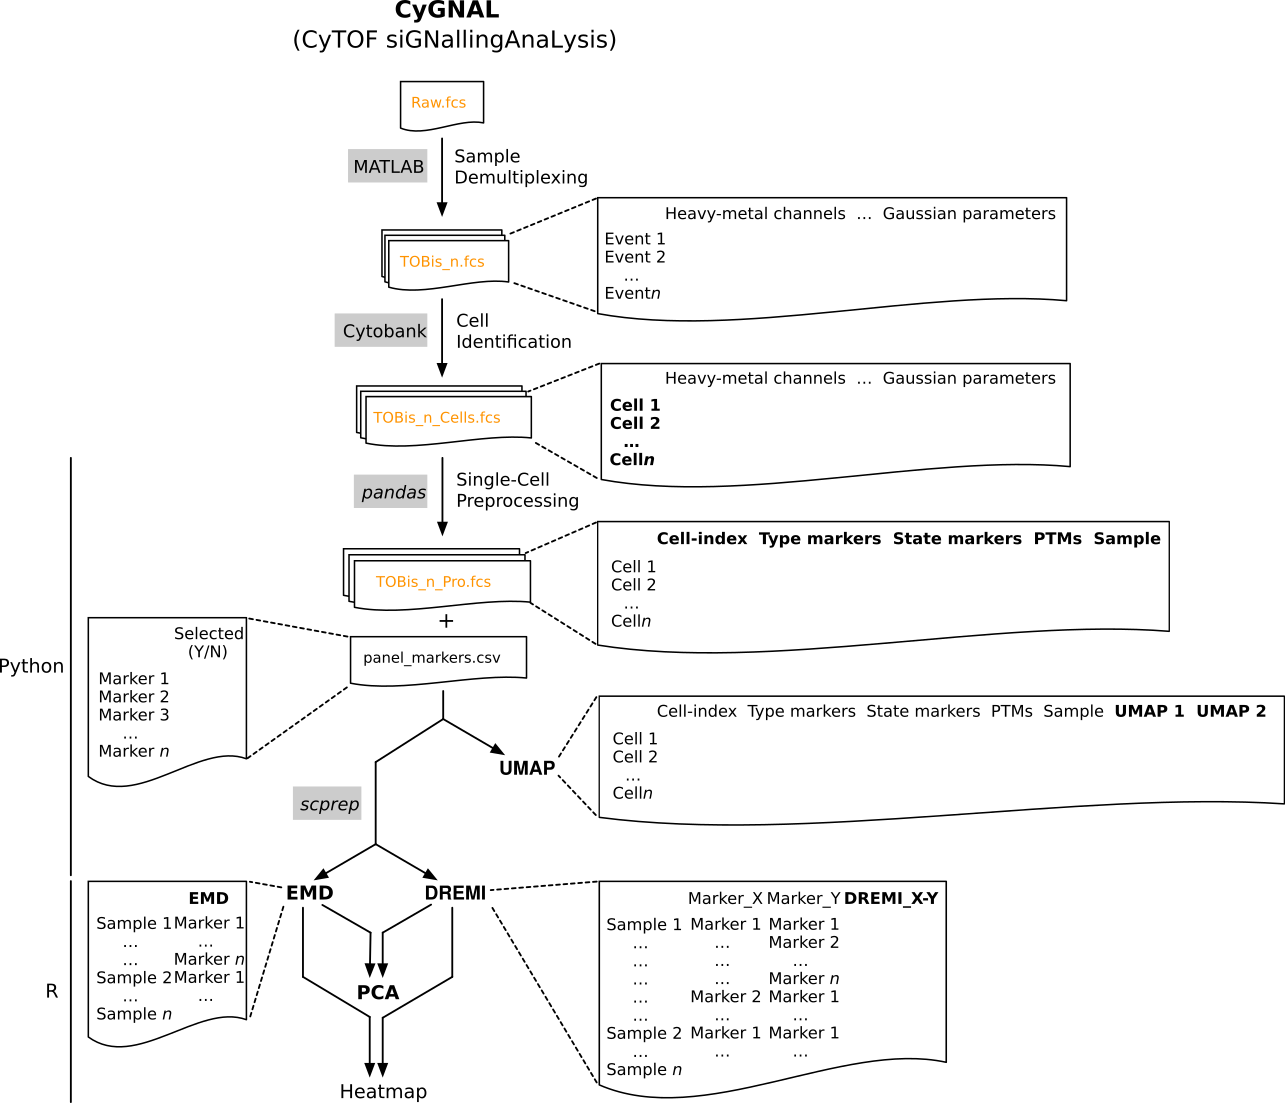
\includegraphics{03cytof/figs/3CYGNAL_pipeline.png}
    \caption{PIPELINE CYGNAL. WIP, consider merging with the use case figure as the overlap is significant.}
    \label{fig:3cygpipe}
\end{figure}

A general overview of CyGNAL's structure is shown in Figure \ref{fig:3cygpipe}, where the tool encompasses the bottom two thirds of the diagram.

As CyGNAL uses FCS files or tab-separated plain text files, certain upstream processes are necessary after data acquisition. Previous to analysing the data in CyGNAL, the standard operating procedure in our lab is to debarcode the mass cytometry datasets in MATLAB (using the tool from \href{github.com/zunderlab/single-cell-debarcoder}{github.com/zunderlab/single-cell-debarcoder}) and perform initial data pre-processing and quality control in Cytobank (\href{www.cytobank.org}{www.cytobank.org}). In that platform, the single cells are gated for Gaussian parameters, their DNA content, and uptake of Cisplatin using manual gates. Gating on cell state and cell type specific markers can also be done in order to both eliminate doublets but also to identify cells belonging to each state or type; information which can then be used to understand the biological system, but also train the cell state classifier.

CyGNAL proper starts with the pre-processing step. Here, empty heavy metal channels with no conjugated antibodies are removed, and the remaining channels are renamed to reduce the presence of special characters and keep with the naming conventions of the Fluidigm CyTOF software. A unique cell identifier is also given to each cell, and experimental metadata can also be embedded within the main pandas dataframe. Furthermore, a file with update antibody channel names is also saved (panel\_markers.csv), so that the user can select which channels to use in downstream steps.

Dimensionality reduction via Uniform Manifold Approximation and Projection (UMAP) \cite{mcinnes_umap_2020} can be performed to embed the individual cells on a 2-dimensional space based on the select antibodies.

EMD and DREMI scores are computed using the scprep package \cite{noauthor_krishnaswamylabscprep_2021}. Compute time can be reduced by subsetting the panel to channels of interest, and the user gets prompted to define specific arguments relevant to either computation, such as defining the variable and reference distributions for the EMD step.

Finally, the computed EMD and DREMI scores can be visualised as heatmaps or further summarised via PCA to compare profiles across conditions using CyGNALs last two main steps. The visualisation steps load in the default and user-given parameters and pass them to R Shiny-Apps \cite{noauthor_rstudioshiny_2021} that host a local server which automatically opens on the browser.

\subsection{Use Case and Outputs}

CyGNAL is distributed with sample mass cytometry datasets, which originate from technical replicates of an organoid monoculture experiment. They have been downsampled so that they can be hosted on GitHub and distributed with the code itself. The results presented in Figure \ref{fig:3cygvis} A-C were generated with this sample data.

In Figure \ref{fig:3cyguse} I present a mass cytometry dataset from Qin \emph{et al.}~\cite{qin_cell-type-specific_2020} to showcase an example use with heterotypic culture conditions where cell type specific analysis is necessary. The data belongs to the same mouse colon organoid model from Chapter \ref{04seq} and presents with a similar experimental setup, wherein organoids with different genotypes where cultured on their own or with macrophages and/or fibroblast cells. Data was subsequently gated and annotated on cell types and states as described above and on the original publication \cite{qin_cell-type-specific_2020}, and then passed onto CyGNAL for preprocessing (Figure \ref{fig:3cyguse} A).

\begin{figure}
    \centering
    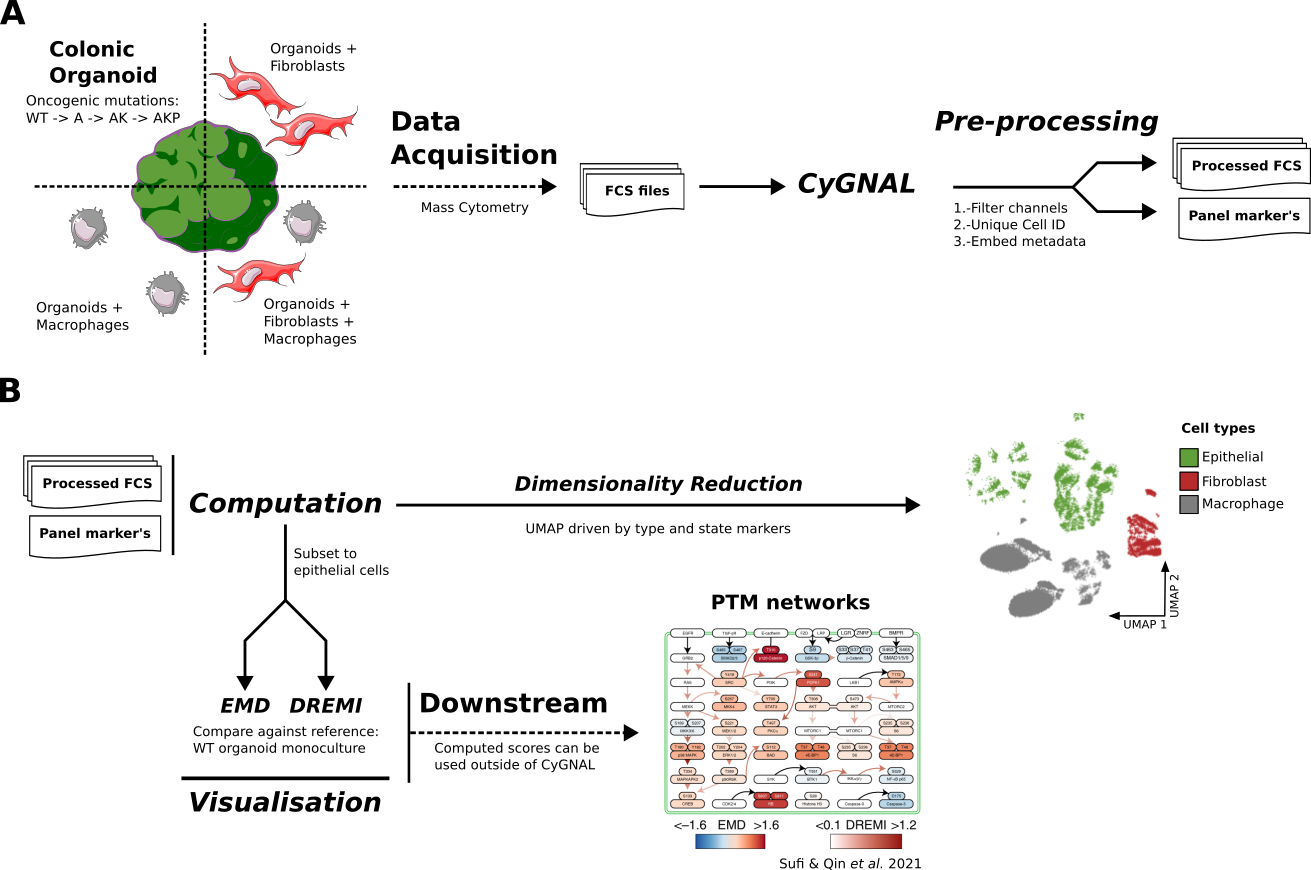
\includegraphics{03cytof/figs/3CYGNAL_usage.png}
    \caption{}
    \label{fig:3cyguse}
\end{figure}

Cell state and type markers were then selected from the panel marker file (pHH3, IdU, cCasp3, pRB, LRIG1, CEACAM1, pan-CK, F4/80, PDPN, RFP, CyclinB1, CD68) from which the UMAP embedding was generated (Figure \ref{fig:3cyguse}B). Embedding resolves the three distinct types (Figure \ref{fig:3cyguse} B).

Using the cell-type gates previously drawn on Cytobank, unique cell identifiers were used to select only the organoid cells. Computation of EMD and DREMI scores was then performed on the epithelial compartment, and can be visualised as part of CyGNAl. Furthermore, in the specific context of PTM network signalling analysis, EMD and DREMI scores can be used to assemble signalling network diagrams. With EMD used to quantify PTM node intensity and DREMI to score PTM-PTM edge connectivity, a signalling network can be curated and manually annotated as shown in Qin \textit{et al}. 2020 \cite{qin_cell-type-specific_2020}. 

When paired with a well-curated antibody panel and robust experimental design, TOBis MC allows multiplexed analysis of cell type–specific PTM signalling of heterocellular organoids \cite{sufi_multiplexed_2021}. 

\begin{figure}
    \centering
    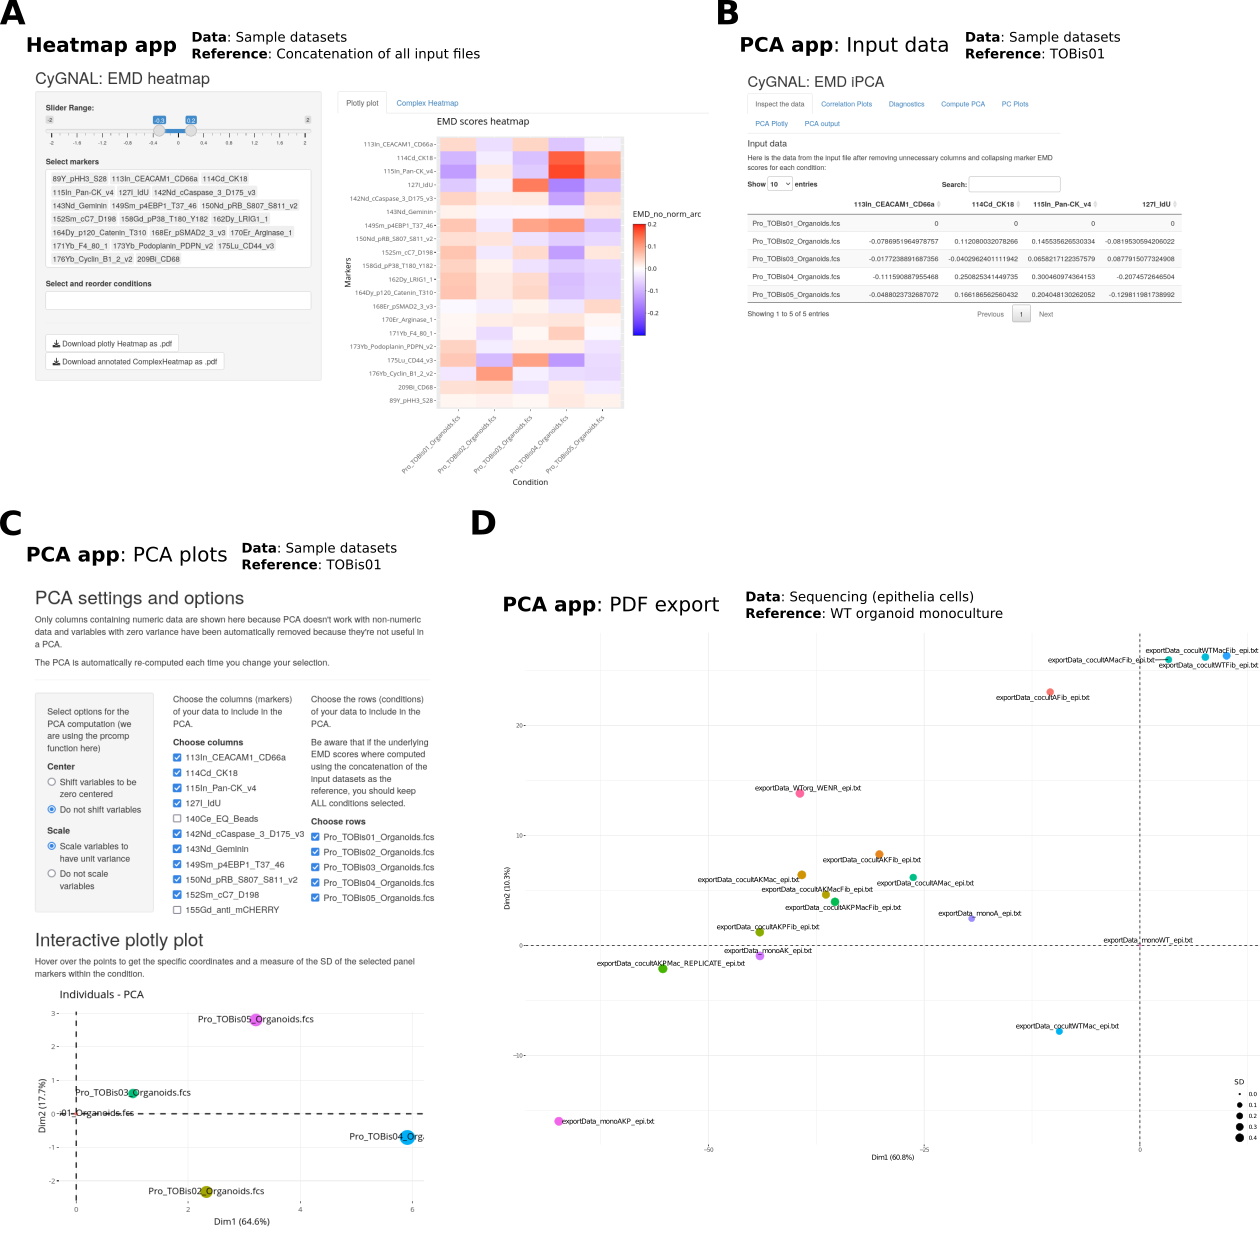
\includegraphics{03cytof/figs/3CYGNAL_usageVIS.png}
    \caption{Manual gates vs Tree vs Forest}
    \label{fig:3cygvis}
\end{figure}

Using the sample data and with the concatenation of all input files as the reference for the EMD step, Figure \ref{fig:3cygvis}A demonstrates CyGNAL's heatmap visualisation. By selecting not to use a specific reference during the EMD computation step, the generated scores are useful to compare how antibody expression compares across each of the individual datasets/conditions. The heatmap ShinyApp lets the user control the colour scale (automatically set to maximise contrast on the range of EMD scores), remove antibodies from the heatmap, and reorder the datasets/conditions shown in the columns. The heatmap shown in Figure \ref{fig:3cygvis}A is an interactive version generated with Plotly \cite{plotly_technologies_inc_collaborative_2015}, and shows the corresponding EMD score when hovering over a cell. Furthermore, a similar non-interactive heatmap is generated using the ComplexHeatmap \cite{gu_complexheatmap_2021} package and can be found within its homonymous Shiny-App tab.

The same data was used when running the PCA Shiny-App in Figure \ref{fig:3cygvis}B-C. This CyGNAL steps lets the user explore the data by looking at the raw scores (Figure \ref{fig:3cygvis}B) and Pearson correlation between channels. The user can also define parameters for the Principal Components Analysis, including the number of markers, generate several types of PCA plots with or without eigenvectors overlaid, and export the PCA results as plain text. In Figure \ref{fig:3cygvis}D I demonstrate how, despite CyGNAL being originally designed to handle mass cytometry data, other types of single-cell omic data like scRNA-seq can also be used. Here I used CyGNAl to compute EMD scores based on the gene expression of the organoids sequenced in Chapter \ref{04seq} and generate a PCA embedding showing how the different conditions compared to the control.
Note that the PCA data in Figure \ref{fig:3cygvis}B-D was generated using EMD scores computed with a particular dataset/condition as the reference and without centring the PCA embedding matrix, exemplifying use cases where we have a clear control condition against with the other conditions are compared (like the WT organoid monoculture in Figure \ref{fig:3cygvis}D).

\newpage
\section{Cell-state Random Forest Classifier}

\begin{figure}
    \centering
    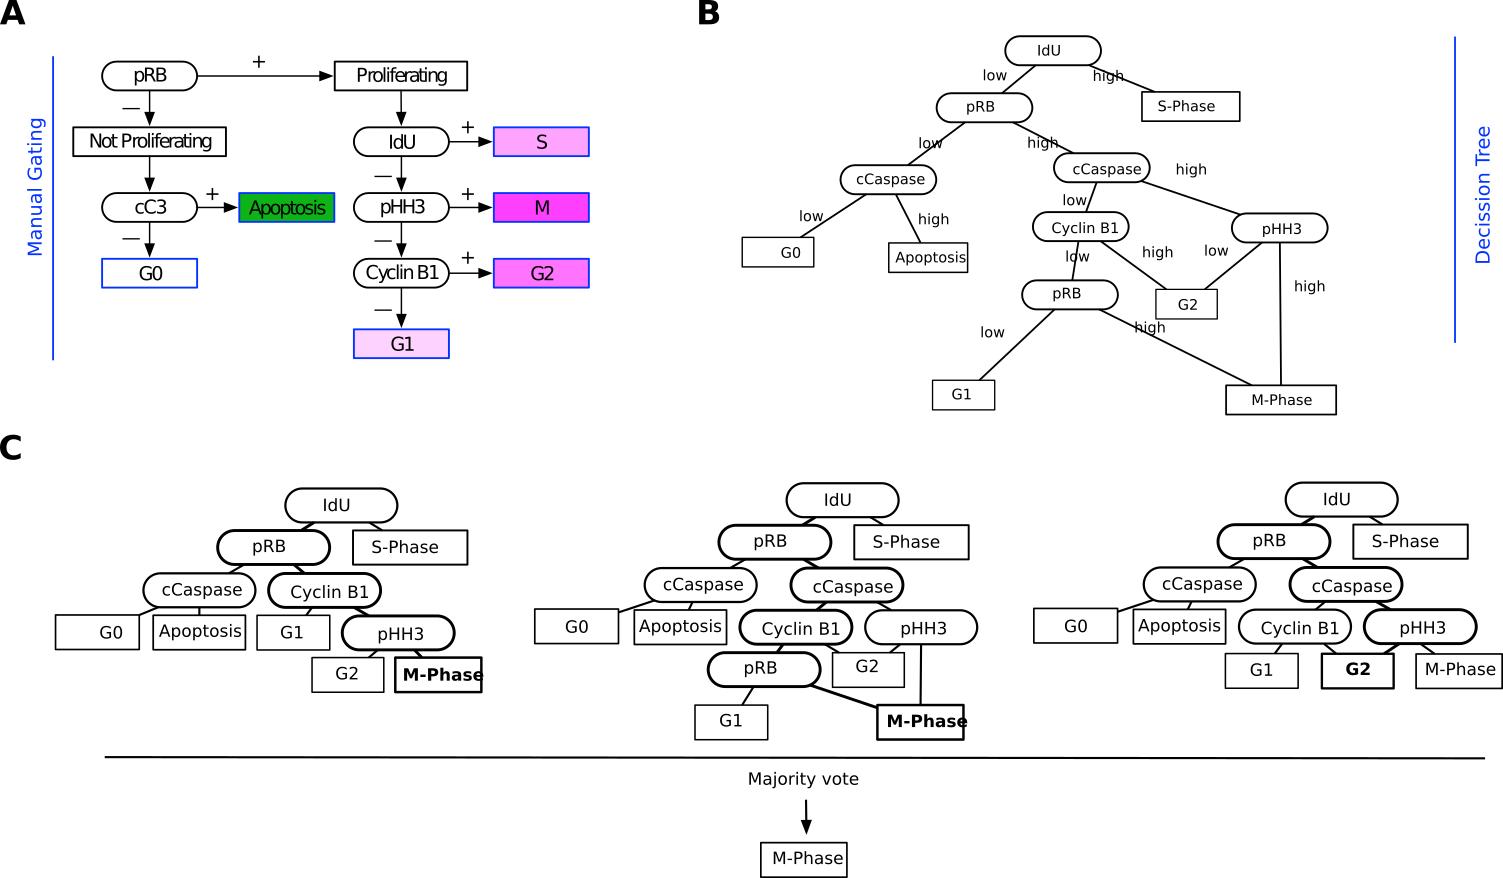
\includegraphics{03cytof/figs/3CLASS_stateRF.png}
    \caption{FINISH THIS FIGURE AND CHANGE COLORS TO MATCH METHODS}
    \label{fig:3classover}
\end{figure}

Determining a cell's state with regards to the cell-cycle phases is central to understanding the intestinal epithelium response to perturbations, as shown by Qin et \emph{al.} and their observations regarding cell-type specific regulation of cell states in response to microenvironmental and oncogenic cues~\cite{qin_cell-type-specific_2020}.

The cell states labels are commonly established using manual gating on a biaxial marker state, wherein a researches draws a boundary separating 2 groups of cells, essentially thresholding the data based on antibody expression. While strategies differ widely, a common approach taken by my lab is depicted in Figure \ref{fig:3classover}A. However, generating these cell state labels is a time consuming process, especially when compounded with the scalability of \acrshort{mc} and TOB\emph{is} ability to perform highly multiplexed analyses. Issues with user-induced biases are also present, as drawing the manual gates is a subjective process that might not remain consistent from experiment to experiment.

Early on my PhD I was exploring the link between \acrshort{ptm}s and cell state when I noticed that the process of generating the cell state labels could potentially be automated using a classical supervised machine learning approach. Eventually thus, I developed a cell state \acrlong{rf} (\acrshort{rf}) classifier to automate this process (see Chapter \ref{02methods} for more details). The manual gating process naturally resembles the logic behind a decision tree, for in both a threshold of antibody intensity would result in a binary classification of cell groups (Figure \ref{fig:3classover}A-B). Furthermore, the \acrshort{rf} machine learning approach remains a white box whose internal decision logic can be easily interpreted, for it consists of a collection of individual decision trees trained on subsets of the data that are used together in an ensemble approach (Figure \ref{fig:3classover}).

\subsection{5-marker model performs across model systems}

\begin{figure}
    \centering
    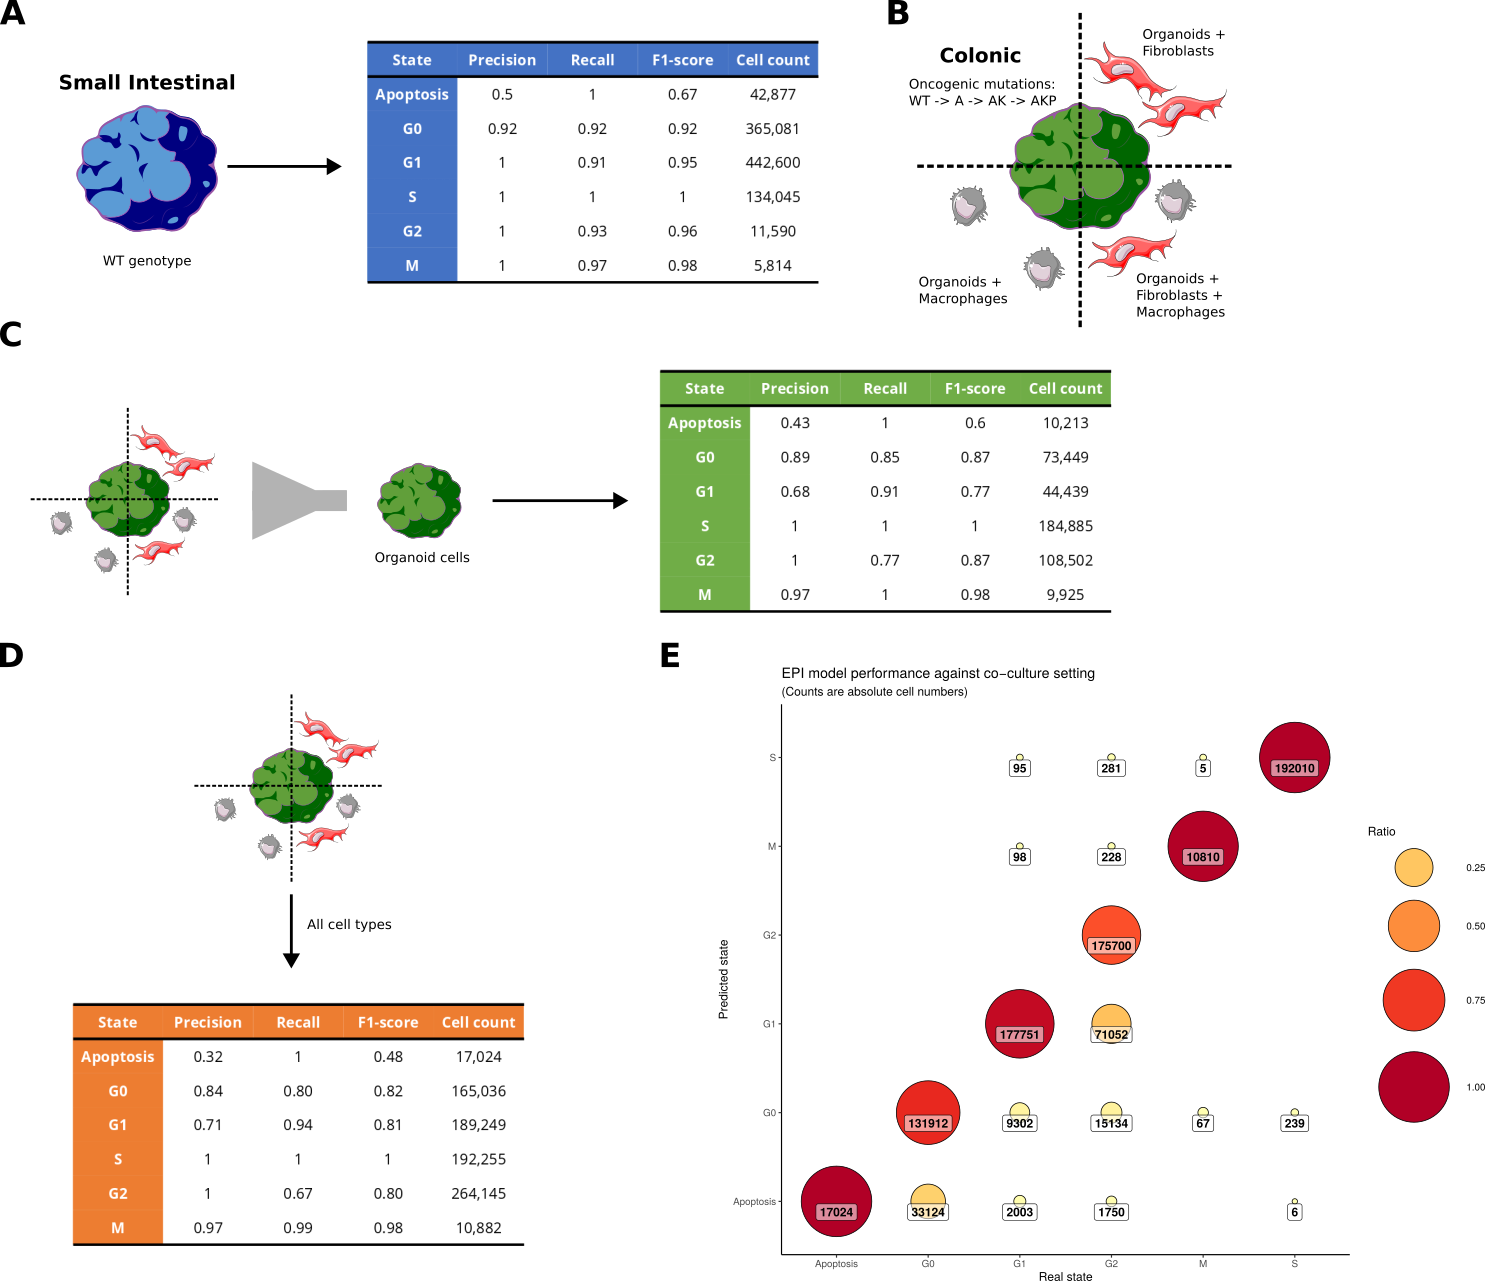
\includegraphics{03cytof/figs/3CLASS_5m.png}
    \caption{Benchmarking 5-marker RF cell state classifier. Shown in a), b), and c) are the classification reports obtained from running the 5-marker RF classifier against data manually labelled for cell state (representing the “real state” or ground truth). In a) a single timepoint SI LGR5 dataset was used, very similar to the training data for the model. The dataset in both b) and c) is a coculture of CRC organoids and their TME, with the cells in b) being a subset of the whole dataset containing just epithelial cells. Decreasing levels of performance correlate with increasing differences between the train and test datasets, as can be seen by the low f1-scores for the apoptotic class in c). Using the same data as c), the dot plot derived from the classification matrix in d) depicts the number and proportion (as both size and colour of the circles) of mislabelled cells for each cell state, showing that a considerable number of falsely mislabelled apoptotic cells are actually in G0 phase and some cells. RF: Random Forest.}
    \label{fig:3class5m}
\end{figure}

The first \acrshort{rf} model built was trained on data from the murine small intestinal organoid cultures from Qin et \emph{al.}~\cite{qin_cell-type-specific_2020}, consisting of \acrshort{wt} organoids along several developmental time points (Figure \ref{fig:3class5m}A). This model used only the 5 markers shown in Figure \ref{fig:3classover}A. Details on building the model and the relative feature importance when training can be found in Chapter \ref{02methods}.

Testing the 5-marker RF model on a different single time-point small intestinal organoid dataset also from Qin \textit{et al}. \cite{qin_cell-type-specific_2020} results in global accuracy for all classes of 0.93. However, $F_1$ scores reveal a big performance drop with the apoptotic class (Figure \ref{fig:3class5m}), driven by the low 0.5 precision score when predicting the apoptotic label. Precision scores otherwise remain above 0.92 for the other labels.

Performance of the classifier drops when testing against the CRC TME colonic organoid cultures from Qin \textit{et al}. \cite{qin_cell-type-specific_2020}. In this case, subsetting just the organoid cells from the organoid cultures (Figure \ref{fig:3class5m}B), we observe a global accuracy of 0.91. Looking at the classification details (Figure \ref{fig:3class5m}C) we see a very similar pattern to the SI LGR5 results; with the apoptotic class presenting the lowest $F_1$-scores (0.6) characterised by a low precision (0.43). Furthermore, the remaining $F_1$-scores are also lower overall, with only the S-phase and M-phase classes reaching above 0.9.

When no epithelial filter is applied to the dataset and the model performance is tested against all cell types (i.e., including also fibroblasts and macrophages) global accuracy drops down to 0.87. The relatively high global accuracy does not reflect the failure of the classifier to, yet again, identify the apoptotic cells (Figure \ref{fig:3class5m}D). In Figure \ref{fig:3class5m}E the classification matrix is used to build a dot plot in which the true labels (“Real state” from gating) are compared against the predicted labels (“Predicted state”), highlighting how a majority of the cells labelled as apoptotic are actually G0 cells, explaining the precision of 0.32 for the former class. There is also some confusion around the G2 cells, as a significant number of these cells are classified as either G0 or G1.

\subsection{10-marker model improves apoptotic classification}

\begin{figure}
    \centering
    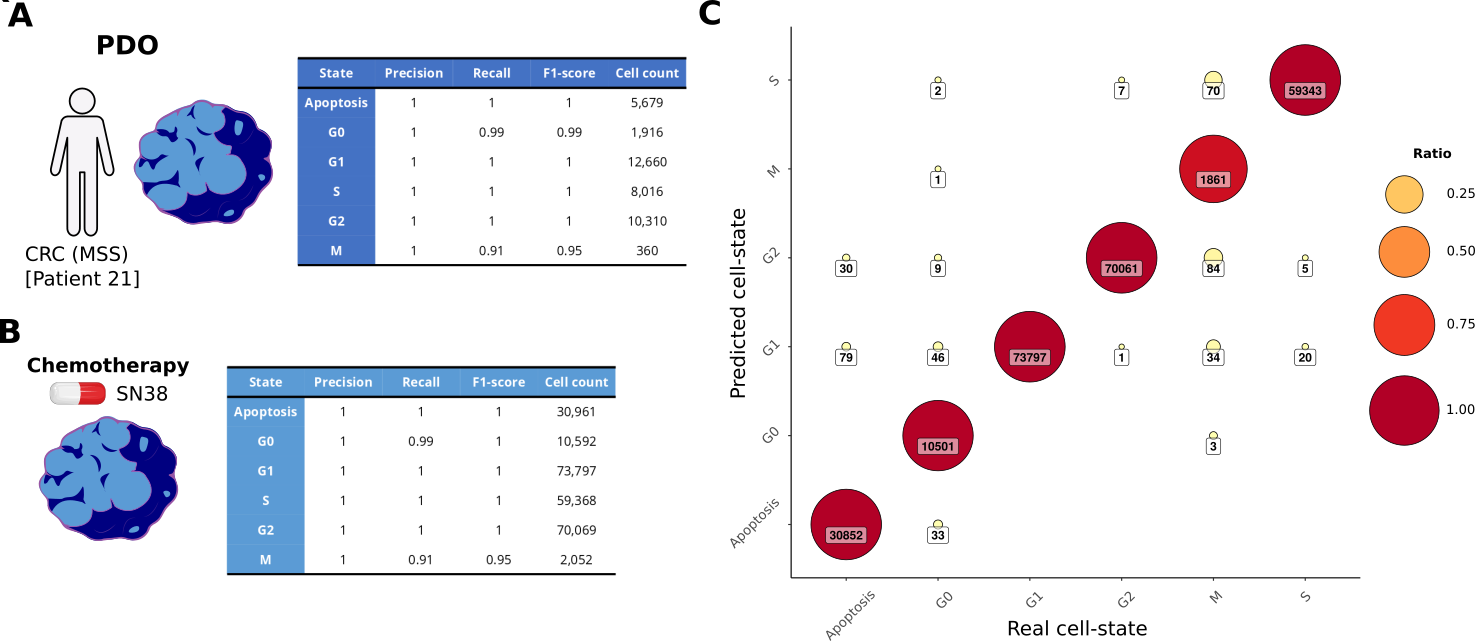
\includegraphics{03cytof/figs/3CLASS_10m.png}
    \caption{Benchmarking the new 10-marker RF cell state classifier. Building a RF classifier with an increased number of markers using data from PDOs renders better results than the original 5-marker model, as can be seen in a) with the classification report. b) Classification matrix generated automatically during model building, showing extremely low levels of misclassified cells. RF: Random Forest. PDO: Patient-Derived Organoids. Labels: 0=Apoptosis, 1=G0, 2=G1, 3=S-phase, 4=G2, 5=M-phase.}
    \label{fig:3class10m}
\end{figure}

Given the 5-marker model limitations when resolving the apoptotic class, I implemented a second model using additional \acrshort{ptm} antibodies and cell state markers targeting apoptotic cells. This 10-marker model uses a dataset from Zapatero \& Tong \emph{et al.}~\cite{zapatero_trellis_2023} wherein heterotypic \acrlong{pdo} (\acrshort{pdo}) cultures from different donors were treated with a spectrum of chemotherapies. This data was generously provided by Dr. Maria Ramos Zapatero.

Results from the updated 10-marker implementation using \acrshort{pdo} data show improved performance when compared to the 5-marker model. Using a technical replicates of the training data as test we observe how the apoptotic class gets accurately resolved (Figure \ref{fig:3class10m}A). When benchmarking the model performance against a dataset wherein the organoid cells had been treated with SN-38, the active metabolite of the type I topoisomerase inhibitor Irinotecan \cite{mathijssen_clinical_2001}, we observe a global accuracy greater than 0.99. The lowest $F_1$-scores, at 0.95, were found for the M-phase label (Figure \ref{fig:3class10m}B). This lowered, yet still accurate, prediction performance is driven by the lower total count of M-phase cells (one order of magnitude smaller than the other classes), hampering the training for that class and resulting in small number of non-apoptotic cells to be miss-labeled as M-phase.
In contrast with the 5-marker model results, there is an apparent lack of issues when classifying the apoptotic class, with only 0.35\% of true apoptotic cells being mislabelled (Figure \ref{fig:3class10m}).

\newpage
\section{Conclusions}

In this chapter I have shown how CyGNAL is an accessible workflow to non-computational users that facilitates data processing and analysis of \acrshort{mc} experiments. The computation of \acrshort{emd} and \acrshort{dremi} scores enables a detailed mechanistic description of changes across conditions, wherein changes in the user defined reference allows for differential interrogation of the experimental system. 

While the scores themselves can be used to build curated mechanistic models as in Qin \emph{et al.} \cite{qin_cell-type-specific_2020}, CyGNAL also incorporates interactive visualisation modules that can automatically plot results. The interactive nature of the visualisation steps, coupled with additional data correlation metrics given during the \acrshort{pca} computation, allows for both exploratory data analysis and (close to) publication grade results generation within a single tool. This same \acrshort{pca} computation presents a straightforward way to summarise changes at the condition level from otherwise information-dense \acrshort{emd} or \acrshort{dremi} heatmaps.

The incorporation of miscellaneous data handling helper scripts in the utilities folder exemplifies how user-provided feedback is paramount, while it also signifies how CyGNAL continuously grows and changes with time. Tools are meant to be used, and that publications by colleagues such as Michelozzi \emph{et al.}~\cite{michelozzi_activation_2023} employed CyGNAL is a testament to its accessibility.

Originally meant as a simple exercise in curiosity-driven exploration after noticing the correlation between so called PTM and "cell state" markers, and empowered by the tediousness of manually gating the datasets in our lab, the \acrshort{rf} cell-state classifier has become a convenient tool to automate cell-state labelling of \acrshort{mc} datasets in relation to cell-cycle phases.

Albeit a very simple model, the nature of the manual gating process (essentially thresholding on a biaxial space of marker expression) translates well to decision trees, and this is shown in the relatively strong overall model performance. The current implementation however, might struggle to generalise to external datasets, for gating strategies are somewhat of a lab- and individual-specific process.

Where we do observe weak points in the classifier is for those cell state labels whose antibody coverage is not great in the model. For example, in the 5-marker \acrshort{rf} model, apoptotic cell class precision reaches only 0.32 in the most stringent setting tested (Figure \ref{fig:3class5m}D). This can be relatively straightforward to address by increasing the number of antibodies targeting that particular state (Figure \ref{fig:3class10m}B-C), but this strategy can not always be employed as the additional marker would both need to be in the reference data used to train the model and in the query dataset to be labelled. When possible however, as demonstrated by the the 10-marker \acrshort{rf} model built, high precision and recall scores are accomplished for all cell states even in the context of cell-cycle disrupting chemotherapy (Figure \ref{fig:3class10m}B-C).

As described in Chapter \ref{02methods}, both tools are publicly accessible in their respective GitHub repositories. 
\chapter{Stromal and Oncogenic Regulation of Colonic Stem Cell Polarisation}
\label{04seq}

\section{Introduction}


AIMS
% Both the SI LGR5 and the colonic organoid systems have been thoroughly characterised before at the mass cytometry level and, to better understand these systems, we aim to perform a comparative characterisation of the organoids using scRNA-seq. 
% Given the well-known biology of the murine small intestine at the transcriptome level21, we can analyse the SI LGR5s to characterise the different subpopulations within the epithelial organoids and cross-validate the results with in vivo scRNA-seq studies and the mass cytometry results discussed above11. In a similar fashion, we also aim to characterise the colonic organoids and the stromal and immune compartments that form the TME in the heterocellular cultures. Unlike mass cytometry, which requires tailored panels of antibodies reaching only into a few dozens, with scRNA-seq we will be able to characterise thousands of genes at once in the organoids, fibroblasts, and macrophages. 
% Leveraging the publicly available ligand-receptor databases mentioned in the background section, data from the scRNA-seq experiments will be used to identify the ligands and receptors expressed in the colonic heterocellular organoid cocultures. 
% The cell communication information gathered this way can then be summarised as signalling pathways that define and connect the different populations of cells. Furthermore, the study of this interactome would aid towards understanding the interplay between the CRC organoid model and its TME. This can be achieved by comparing the cell communication results with the intracellular PTM signalling described in Qin et al. 2020 and seeing how cellular communications change in cultures mimicking an oncogenic setting.

\subsubsection{Figure on experimental design, with the 2 axes of perturbation}

\section{Organoids recapitulate colonic epithelial cell states}

\subsubsection{Figure on Integrated object DR, and expression of cannonical markers in control condition}

\section{Oncogenic mutations and fibroblasts polarise epithelia towards distinct stem cell fates}

\subsubsection{Figure on DA overview and individual DA tests}

\subsubsection{Figure on signalling entropy, RNA velocity changes, and CellRank sinks}

\section{Oncogenic mutations block fibroblast to epithelia signalling}

\subsubsection{Figure on cell-cell communication analysis}

\section{Characterisation and relevance of proCSC and revCSC}

\subsubsection{Figure on stem signatures and key signalling pathways}

\section{Conclusions}






\chapter{Data-driven Landscapes of Colon Epithelial Plasticity}
\label{05vr}

\section{Introduction}

More than 60 years ago, Conrad H. Waddington illustrated the process of an epigenetic landscape where pluripotent cells would roll down into valleys of terminally differentiated states\cite{ch_waddington_waddington_1957}. Albeit a powerful image of developmental biology, his effort and subsequent ones since then have mostly been of a rather subjective and artistic nature. Reconstructing such landscapes from biological data is not an untenable task anymore, as \emph{omic} profiles from single-cells can be embedded together and mapped onto a 3D space sculpted by cellular pluripotency metrics \cite{chen_single-cell_2019}.

However, none of those methods appear to leverage embeddings able to capture transitional processes and global structure. Furthermore, such as Waddington-like landscape is not only informed by the overall elevation, but also by more local features that determine the presence of troughs and valleys and thus limit the repertoire of likely transitions downhill.

Here I propose a novel method to generate such data-driven Waddington-like landscapes using; 1) embeddings that capture global structure (PHATE \cite{moon_visualizing_2019}), 2) a cellular pluripotency metric to derive coarse landscape elevation (CCAT \cite{teschendorff_single-cell_2017}), and 3) RNA velocity metrics to capture local transciptomic changes (scvelo \cite{bergen_generalizing_2020}) that inform state accessibility (Figure \ref{fig:5land}A).

This work has been published as part of Qin \& Cardoso Rodriguez \emph{et al.}~\cite{cardoso_rodriguez_single-cell_2023}, and the code to compute the VR score and generate the landscapes is publicly available as a Jupyter Notebook on \url{github.com/TAPE-Lab/Qin-CardosoRodriguez-et-al/blob/main/Figure7_S7/Landscape.ipynb}. 

\section{The Valley-Ridge Score}

\begin{figure}
    \centering
    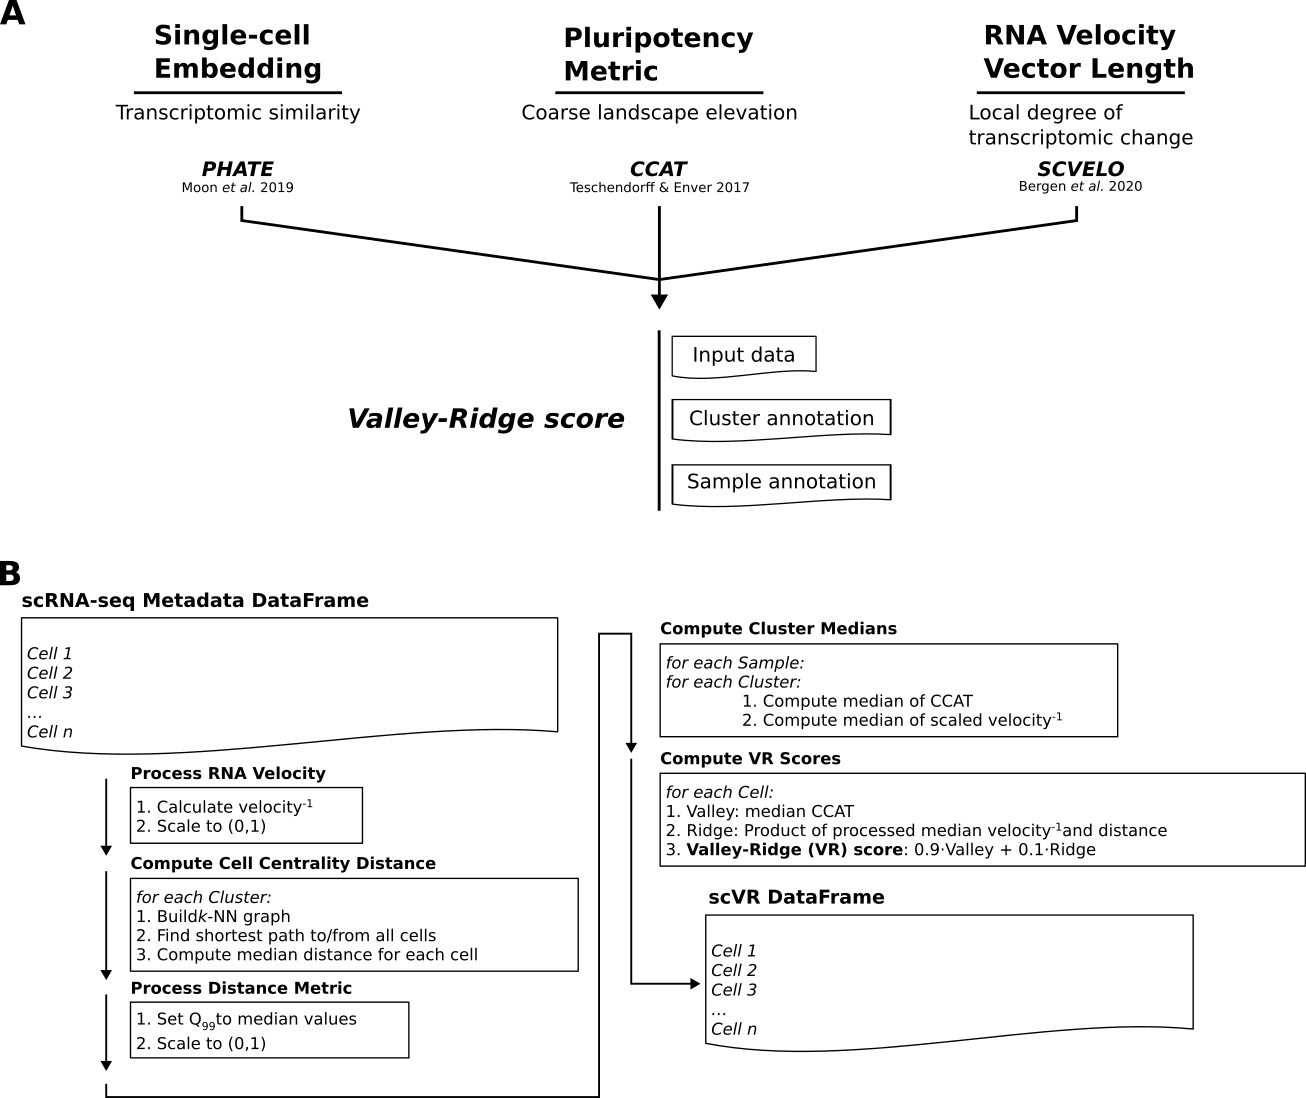
\includegraphics{05vr/figs/5VR_score.png}
    \caption{\textbf{Workflow for calculating VR scores from scRNA-seq data}. \textbf{A)}. \textbf{B)}.}
    \label{fig:5score}
\end{figure}

Following with the geographical analogy, the PHATE space would act as the \emph{longitude} and \emph{latitude} coordinates whereas we need to define a new metric that combines both CCAT scores and RNA velocity vector lengths. This metric has been called the Valley-Ridge (VR) score, in reference of its two components that respectively inform macro-level and hyper-local features of the landscape (Figure \ref{fig:5land}A).

While these two metrics have already been discussed previously in this work, here is a small summary of what they entail. CCAT has been defined as an estimate for a cell's Signalling Entropy Rate, which has been shown to be a robust metric for cellular pluripotency \cite{teschendorff_single-cell_2017,chen_single-cell_2019,senra_origins_2022}. RNA velocity vector lengths are the modulus of the inferred RNA velocity vectors as determined by a cell's ratio of spliced and unspliced mRNA, thus measuring the overall rate of transcriptomic change undergone by a cell.

Detailed information on the definition and computation of the VR score can be found in Chapter \ref{02methods}. In brief, the VR score is a cellular metric computed on a per sample and cluster labels and is defined as the weighted sum of the two components: CCAT signalling-entropy \cite{teschendorff_single-cell_2017} and RNA velocity vector length\cite{bergen_generalizing_2020} (Figure \ref{fig:5land}B). 
At a cluster's centre, the VR score is solely determined by the median CCAT. However, the VR scores at the cluster periphery are augmented by weighting the inverse of RNA velocity component and the scaled distance from the cluster centre to model rates of local transcriptional change. We use the inverse of the velocity vector length so that transitions substantiated by high RNA velocities do not locally increase landscape elevation at a cluster's boundary, with the opposite happening for low velocity cells.

This method thus reconstructs a data-driven estimate of Waddington-like landscapes where the overall altitude captures the differentiation potential of a cell population, with the valley-ridge topology delineating local plasticity and cell state availability. 

\section{Landscapes of Colonic Epithelia Cell-fate Plasticity}

Having been described in Chapter \ref{04seq} and in Qin \& Cardoso Rodriguez et al. 2023, the heterocellular murine colonic organoid system represents a suitable candidate to test the VR landscapes. 
This system consists of colon epithelia organoids increasingly accumulating canonical CRC oncogenic mutations, and with various combinations of microenvironmental perturbations including a stromal component (Figure \ref{fig:5land}A).

The cellular dynamics of this system point towards stromal cues differentially polarising the colonic epithelia towards a \acrshort{revcsc} state, less proliferative and with lower pluripotency scores than the other stem states. There is also some degree of loss of terminally differentiated states by stromal cues, specially around the absorptive compartment, but this de-differentiation was not as pronounced as in CRC organoids.
The oncogenic mutations in CRC organoids polarise the epithelia to the proliferative and highly pluripotent (as determined by CCAT) \acrshort{procsc} state. Furthermore, RNA velocity vector lengths in CRC organoids were greatly reduced when compared to the other genotypes (Figure \ref{fig:4dyn}C-D), suggesting that normal transitional processes within the epithelia are impeded by oncogenic mutations.
The VR score is a way of visualising all of these processes at once by generating a purely data-driven VR landscape reminiscent of Waddington own's drawing.

\begin{figure}[h]
    \centering
    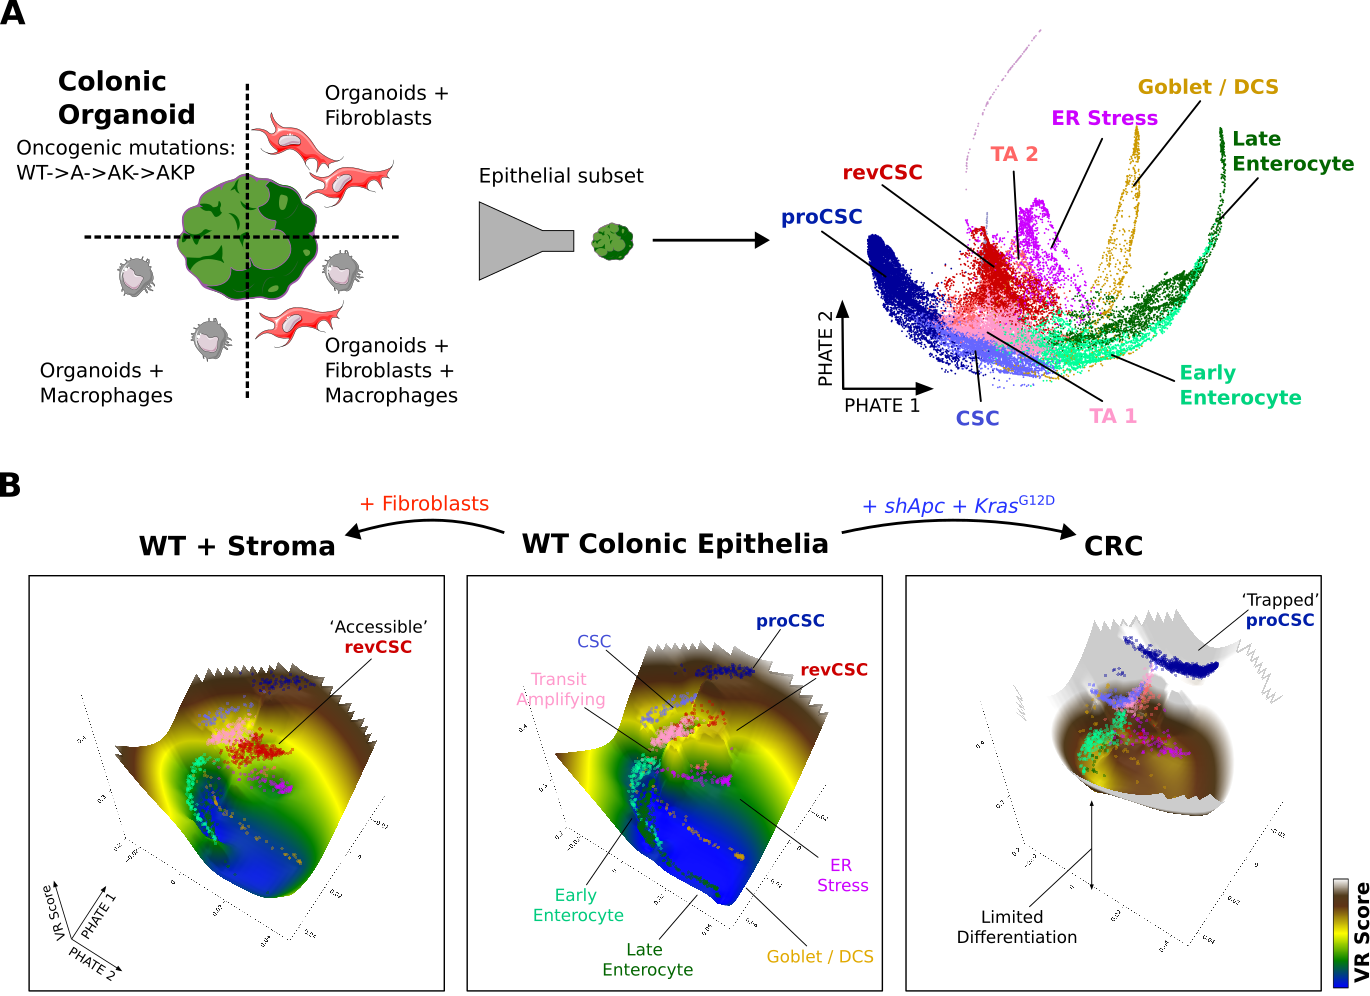
\includegraphics{05vr/figs/5VR_landscape.png}
    \caption{\textbf{Fibroblast- and Oncogene-driven Waddington-like Single-cell Landscapes.} \textbf{A)} Setting/data. \textbf{B)} Integrating PHATE and Valley-Ridge (VR) score enables Waddington-like embeddings of scRNA-seq data. Landscapes illustrate how WT epithelia differentiate from high signalling-entropy stem cells, through TA cells, into secretory and absorptive cells. Fibroblasts enable WT epithelia to access revCSC while retaining secretory and absorptive differentiation. In contrast, \textit{shApc} and \textit{Kras\textsuperscript{G12D/+}} limit differentiation and trap cells in the proCSC state.}
    \label{fig:5land}
\end{figure}

When WT colonic epithelia are projected onto this embedding, stem cells occupy high positions in the landscape, with TA cells descending into a central valley before diverging into terminally differentiated secretory and absorptive cells (Figure \ref{fig:5land}B). When WT epithelia communicate with fibroblasts, the TA valley erodes as cells access revCSC (Figure \ref{fig:5land}B). In contrast, CRC mutations \textit{shApc} and \textit{Kras\textsuperscript{G12D/+}} re-sculpt the entire landscape, trapping most cells in the proCSC fate by restricting their differentiation potential (Figure \ref{fig:5land}B). 

This landscape projection exemplifies the VR score profile of cellular states such as proCSC, which are highly pluripotent (Figure \ref{fig:4dyn}B) yet static states in terms of rate of transcriptional change (Figure \ref{fig:4dyn}C). These sates appear as high elevation tarn-like features, areas of high elevation surrounded by an obstructive ridge that symbolises the low likelihood of transition towards surrounding states.

See Chapter \ref{02methods} for details on the methods used to interpolate the VR scores into a surface and the pipeline to generate the VR landscapes (Figure \ref{fig:2land}).

\newpage
\section{Conclusions}

The VR score presented here synthesises two orthogonal metrics (signalling entropy rate and transcriptomic rate of change) that when combined are very useful in visualising transitional processes and plasticity of a system. 

The multi-scale nature of the its components, with CCAT determining coarser cluster-level features and RNA velocity vector lengths more local inter-cluster transitions, proves useful when reconstructing data-driven Waddington-like landscapes. 

When applied to murine organoid perturbation system from Chapter \ref{04seq}, the VR landscapes depict a picture of a shared differentiation landscape that can be traversed through cell-extrinsic ligands or cell-intrinsic oncogenic mutations. In particular, the increased availability of \acrshort{revcsc} in the presence of stromal ligands (Figure \ref{fig:4da}) can also be observed on the VR landscapes (Figure \ref{fig:5land}B). Furthermore, the collapse of stromal-to-epithelial communications in cancer organoids (Figure \ref{fig:4cc}A) and their lack of \acrshort{revcsc} polarisation (Figure \ref{fig:4da}C) is reflected in the tarn-like topology of the AK VR landscapes, where the bulk of the organoid appears trapped in the \acrshort{procsc} state.

By combining the VR score computation and landscape projection into a single easy to use notebook, I have laid the foundation towards future packaging and deployment of this tool as an interactive service. By the name of VRland, this tool is currently available as an annotated Jupyter Notebook in the code repository for Qin \& Cardoso Rodriguez \emph{et al.}~\cite{cardoso_rodriguez_single-cell_2023} (\href{www.github.com/TAPE-Lab/Qin-CardosoRodriguez-et-al}{github.com/TAPE-Lab/Qin-CardosoRodriguez-et-al}).

\chapter{Knowledge Graphs for Cell Communications}
\label{06kg}

\newpage
\section{Introduction}

\begin{figure}
    \centering
    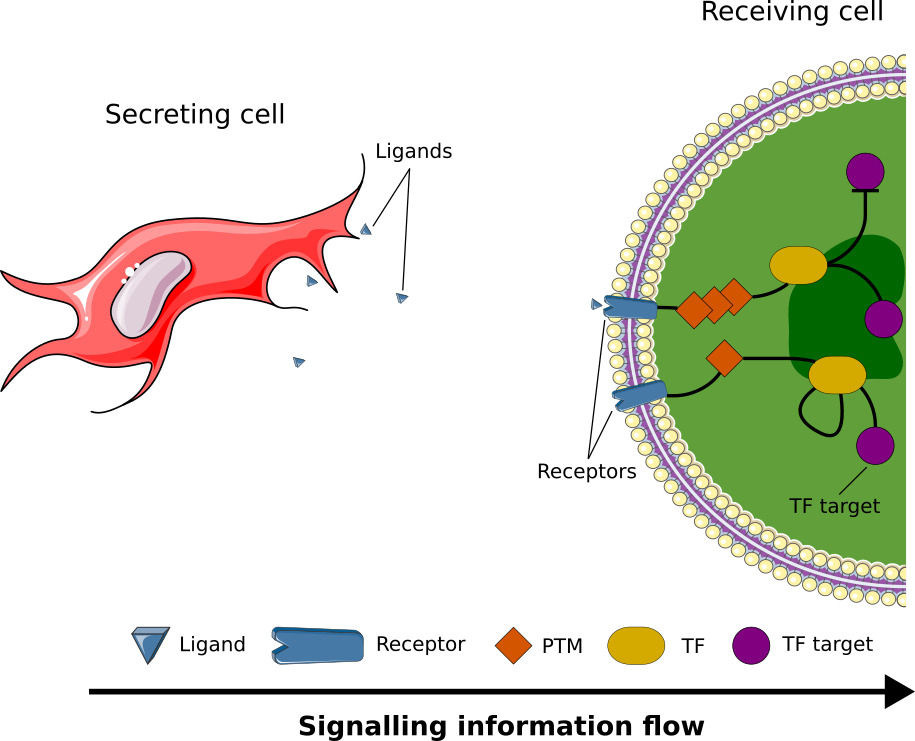
\includegraphics{06kg/figs/6KG_com.png}
    \caption{}
    \label{fig:6intro}
\end{figure}

Cellular signalling involves a complex series of directed and hierarchical~\cite{kumar_3_2003} signal transduction cascades between molecules that dictate a cells response to extrinsic and intrinsic cues. In the context of inter-cellular paracrine communication, a secreting cell produces a series of ligands that are captured by receptors on a receiving cell. The receiving cell then might engage in an intra-cellular signal transduction cascade orchestrated by \acrshort{ptm}s, such as the MAPK cascade~\cite{zhang_mapk_2002}. These cascades regulate gene expression downstream of active transcription factors. With overlapping pathways, feedback loops, and complex settings with multiple cells engaging in symmetrical or non-symmetrical communications, there is nonetheless a directional causality-driven signalling information flow (Figure \ref{fig:6intro}). This directional nature can be measured in terms of graph hierarchy scores, and to aid with that purpose I have developed a python package to compute such scores (Appendix \ref{appendix:pykrack}).

The physical interactions between molecules are often represented as a network of genes, proteins or even \acrshort{ptm}s, described in the manner of a \acrfull{kg}. These network representations have been extensively explored to model both intra- and inter-cellular communications, but to date they are not consistently analysed using methods that leverage the underlying directed and hierarchical nature of signalling processes, often either treating the graph as undirected or analyzing pairwise relationships between feature detection metrics (such as gene expression)~\cite{pratapa_benchmarking_2020, armingol_deciphering_2020}. 
    % Cellular signaling involves overlapping directed \cite{HANCOCK200364} and hierarchical signal transduction cascades between molecules to coordinate targeted behavior \cite{zhang_mapk_2002}.
    % %The physical interactions of molecules are often represented as a network.
    % The resulting network of molecular interactions determines a cell's response under different conditions, drawing interest towards unifying and characterizing varying sources of molecule signaling from distinct scientific experiments. However, methods to represent biological networks and infer gene-gene relationships rarely take into the account the \textit{directionality} and \textit{hierarchical structure} of these gene graphs.

The field of directed cellular interaction databases already presents with some established curated resources like OmniPath~\cite{turei_integrated_2021}, with a growing number of methods attempting to model communication in a directed manner~\cite{lefebvre_large-scale_2021}, describing cell-cell interactions~\cite{fischer_modeling_2022,yang_sctenifoldxct_2023}, and even data-driven \emph{de novo} generation of signal transduction networks~\cite{hu_cytotalk_2021}.

In this chapter I propose a novel approach for assembling gene-gene graphs that capture cellular communication by leveraging \acrshort{kg} embedding approaches, which would allow for the encoding of the original directed \acrshort{kg} into a simpler non-directed format amenable to downstream analysis and data projection. I aim to project single-cell \emph{omic} profiles into the assembled \acrshort{kg}s, thus treating the cells as signals on a gene graph. The resulting signals can then be considered as another single-cell \emph{omic} view of the cells, and used to generate new embeddings or be compared against their gene expression profiles.

        % Gene embedding methods are growing , so are graph signal processing approaches. 
        % Discuss the embedding methods of these graphs:
        % Complexity in terms of structure, directionality and type of interaction. All of this is very important, unlike in undirected knn grpahs ubiquitous to omic analyses.
        % This means that we need some methods able to compute all of this complex relations in multi relation directed graphs  (MultiDiGraph). methods have been developed, transE \cite{bordes_translating_2013}family, graph convolutional networks, and the stuff from he stanford dawn group on  hyperbolic embeddings  \cite{chami_hyperbolic_2019} and general ML approaches applied to non euclidean spaces.
        % Non-euclidean space like hyperbolic spaces argued to be key because graphs with important hierarchical structure [as is biological signalling] is much better capture in a hyperbole than in a plane \cite{bronstein_geometric_2017,nickel_poincare_2017,chamberlain_neural_2017}.[the first one is general Euclidean =bad, the later ones refer to the cocnept of hierarchical graph better on hyperboles than planes].
        % on the other hand, prelim results in collab porject suggest perhaps not as important for bio KG despite the hierarchical nature of signalling networks.



\section{A KG for Ligands, Receptors and TF Targets}

\begin{figure}
    \centering
    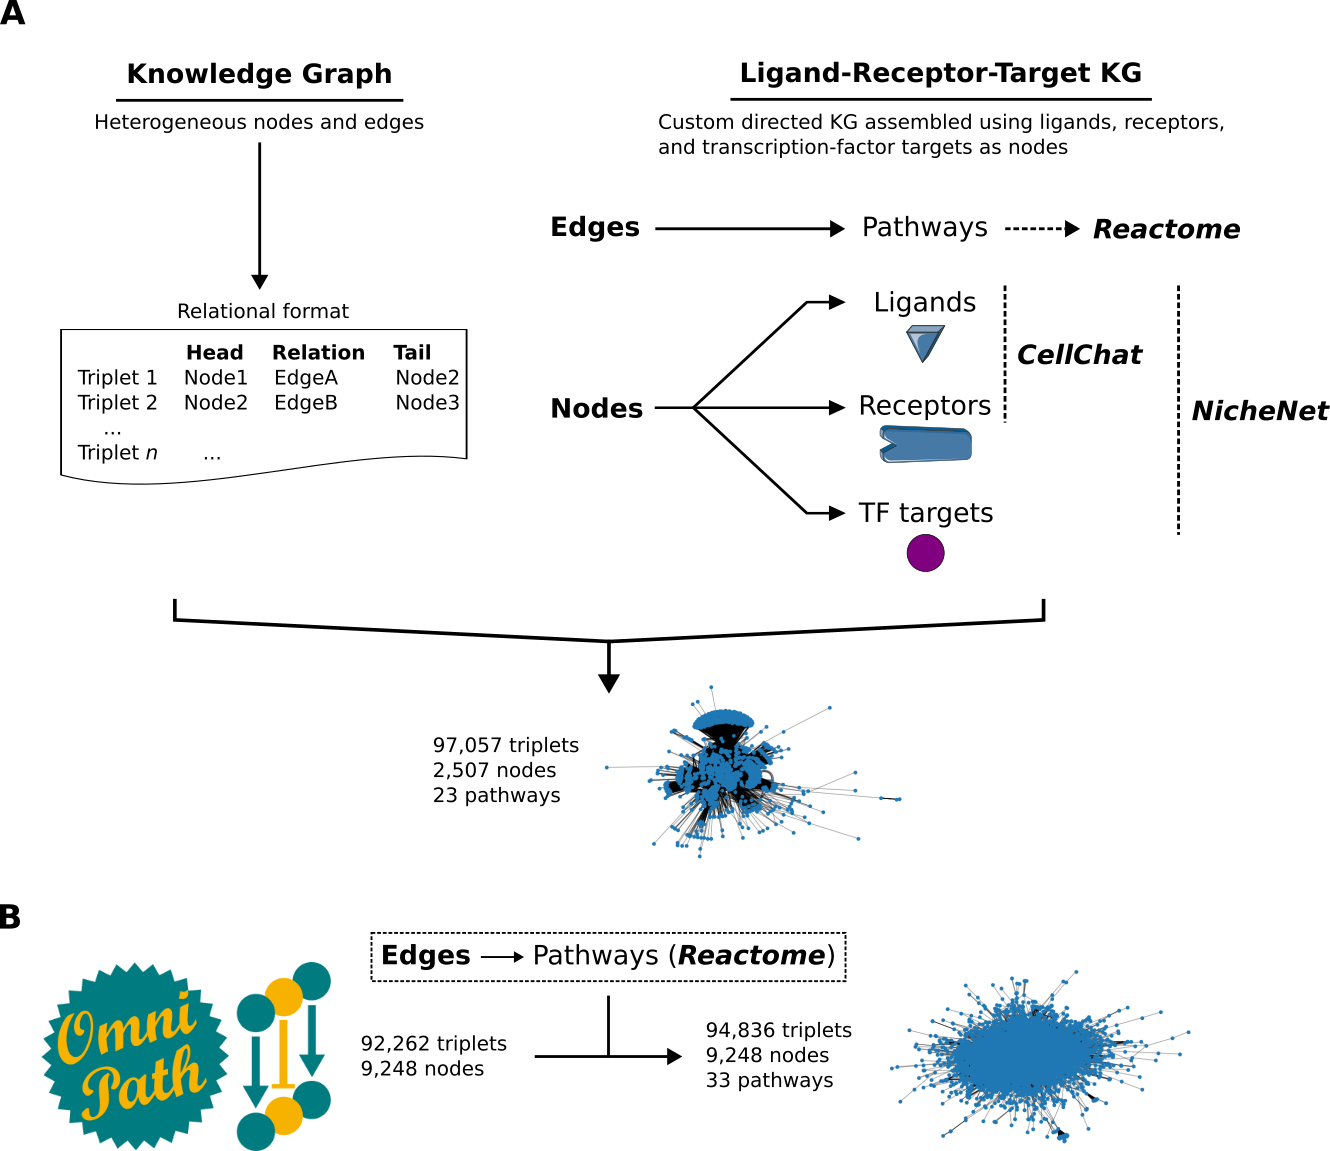
\includegraphics{06kg/figs/6KG_kg.png}
    \caption{}
    \label{fig:6kg}
\end{figure}

Literature information on cell communication interactions is commonly found in the form of databases used for cell-cell communication analyses, and not in a directed graph format. Therefore I assembled a custom \emph{kg} from public databases and compared it with OmniPath~\cite{turei_integrated_2021}, an existing curated repository of directed inter- and intra- cellular signalling interactions. More details on this process can be found in Chapter \ref{02methods}.

I gathered information from the CellChat~\cite{sqjin_sqjincellchat_2021} and NicheNet~\cite{browaeys_nichenet_2020} databases to assemble a directed \acrshort{kg} wherein nodes are genes for ligands, receptors or \acrfull{tf} targets (Figure \ref{fig:6kg}). This \acrshort{kg} aims to capture inter- and intra-cellular communication; with ligand and receptor nodes describing the relationship between interacting cells, and the \acrshort{tf} targets capturing cellular states and response to stimuli.

Following the ubiquitous triplet format, I thus encoded the graph as a relational database where pathways from Reactome~\cite{gillespie_reactome_2022} were used to annotate and relate the different gene nodes (Figure \ref{fig:6kg}).

The resulting ligand-receptor-target \acrshort{kg} (\acrshort{lrtkg}) has over 2,500 nodes linked by interactions belonging to 23 distinct pathways. To validate broad-scale graph characteristics this custom graph was compared against the OmniPath resource.
The OmniPath database has multiple layers of relational information between genes (and other molecules such as \acrshort{ptm}s), including directionality, supporting evidence and functional information on the nature of the interaction (i.e. activation or inhibition of receiving interaction member). Assembled in the same manner as the LRT-KG object, the OmniPath graph presented with a higher number of gene nodes and pathways but comparatively less interactions  and a lower hierarchy score than the LRT-KG (Figure \ref{fig:6kg}B and Table \ref{tab:2kg}).


\section{KG Embeddings Preserve Graph and Biological Information}

\begin{figure}
    \centering
    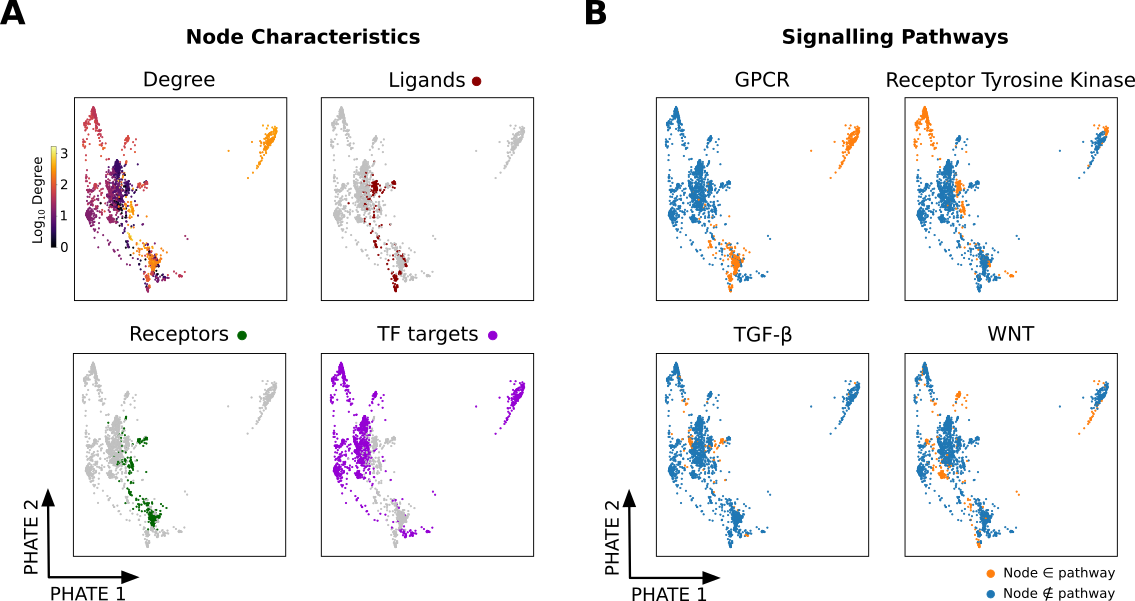
\includegraphics{06kg/figs/6KG_embed.png}
    \caption{XXXXXXXXXXX}
    \label{fig:6embed}
\end{figure}

To capture the complex relational information in a simpler format amenable to downstream analyses, directed heterogeneous knowledge graphs can be embedded into low dimensional tabular representations. Methods like the classical TransE~\cite{bordes_translating_2013} and its derivatives, graph convolutional networks, and hyperbolic embeddings~\cite{chami_hyperbolic_2019}, represent some of different approaches to learn the structure of \acrshort{kg}s.

I used the TransR method~\cite{zhang_transr_2021} to embed the LRT-KG into a 50-dimensional space (Chapter \ref{02methods}), whose PHATE representation suggests that the embedding method captures topological differences between the distinct node types in the graph (Figure \ref{fig:6embed}A). Node degree also seems to drive some of the topology in the PHATE representation of the embedding, and it would appear that TF targets are the most promiscuous nodes with higher degrees, followed by receptor nodes and finally ligands (Figure \ref{fig:6embed}A). However, care must be taken when making these comparisons for three node classes are imbalanced.

Functional biological information encoded by the edges seems to also be captured in the embedded graph. Signalling pathways belonging to the Signal Transduction category in Reactome, which should cover all three types of node in the LRT-KG, were mapped to gene node embedding. The resulting distribution of pathways, occupying discrete and specific regions of PHATE representation (Figure \ref{fig:6embed}, appears to suggest that relational information from the \acrshort{kg} is also conserved in the 50-dimensional embedding.

% Finally, embedding representation of relations (edges) can be generated, which should capture relations between pathways. Recover high level groupins of pathways with similar biological function, due to their shared nodes on KG.
%     WE can also check out the different pathawys they belong to and see if there is come kind of biologically driver distribution here re pathways. Edges can also be embedded and hopefully lowere level pthawys belonging to a shared bigger levl pathways might lie in closer together? Also deppening on the ratio of shared interactions members between disticnt pathways. 

\section{Projecting Cells as Signals on the KG}

\begin{figure}
    \centering
    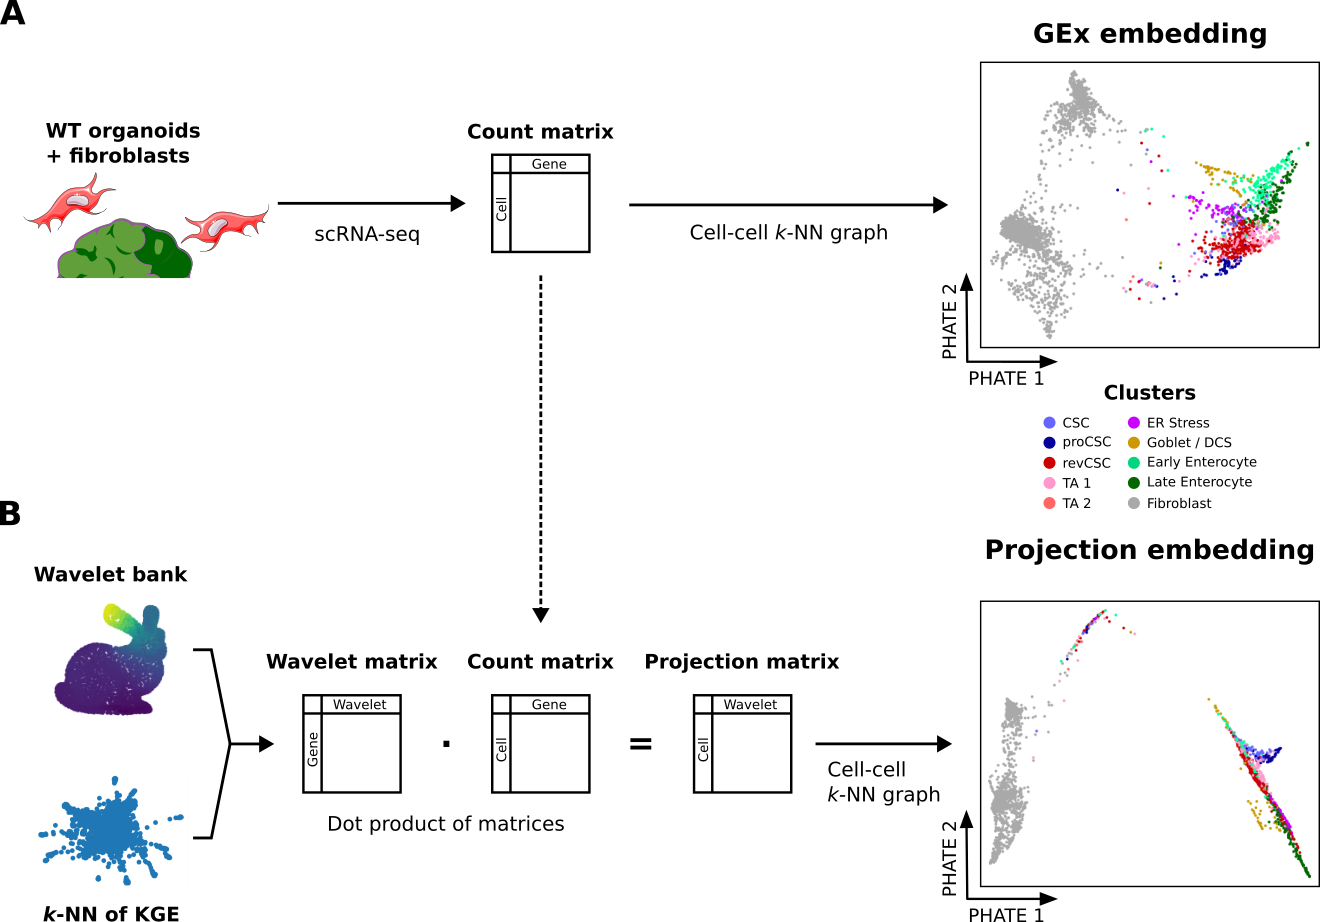
\includegraphics{06kg/figs/6KG_projection.png}
    \caption{XXXXXXXXXXXXXX}
    \label{fig:6project}
\end{figure}

Using a WT organoid and fibroblast co-culture scRNA-seq dataset from Chapter \ref{04seq} (Figure \ref{fig:6project}A) I could explore the usefulness of the LRT-KG embedding to describe a cell's \acrfull{gex} profile as projected on a cell communication graph. 

That particular dataset was employed because I had previously established, using cell-cell communication analysis tools and subsequent \acrshort{mc} validation by Dr. Xiao Qin~\cite{cardoso_rodriguez_single-cell_2023} (see Chapter \ref{04seq} for Figure \ref{fig:4cc}A), that the fibroblast cells engage in active communication with the organoid cells, in particular toward the \acrshort{revcsc} state and adjacent areas of the colonic stem compartment. 

When the transcriptomic data is used to generate a PHATE embedding the two distinct cell types are easily resolved, and so are the heterogeneous cell states within the colonic organoid epithelia (Figure \ref{fig:6project}A).

To project these cellular \acrshort{gex} profiles on the LRT-KG I first applied a diffusion wavelet transform to a \emph{k}-NN representation of the LRT-KG embedding, thus generating a \(node X wavelets\) matrix where the first axis corresponds to the gene nodes of the LRT-KG (Figure \ref{fig:6project}B). 

Leveraging the shared feature axis between the \(node X wavelets\) and scRNA-seq \(cell X gene\), I used the dot product (\(\cdot\)) operation to project the transcriptomic data as a \(cell X wavelets\) matrix representation (Figure \ref{fig:6project}B). The projected data can be treated as the scRNA-seq count matrix from above to compute cell-cell \emph{k}-NN graphs and two-dimensional embeddings.

The resulting projection seems to non-quantitatively resemble the \acrshort{gex} profile on a PHATE space, wherein cell type is easily resolved. There appears however that there is some signal loss during the projection process, for epithelial heterogeneity is reduced (Figure \ref{fig:6project}B). 

To quantitatively asses the projection results I not only compared it with the \acrshort{gex} data but also with the interaction strength predictions between cluster pairs in the data (see Chapter \ref{02methods} for more details). 

Average distances between cluster pairs in the LRT-KG projected space and the \acrshort{gex} space where computed based on their \emph{k}-NN representations (Figure \ref{fig:6bench}A) and found to be highly correlated (Figure \ref{fig:6bench}B). A weak positive correlation (\emph{R} = 0.42) between interacting cluster pairs and their distances is thus observed both in the \acrshort{gex} and highly similar projected spaces (Figure \ref{fig:6bench}C).

Finally, the inter-cluster distance matrices (Sup. Tables \ref{tab:kgdistge} and \ref{tab:kgdistlrt}) were scaled and subtracted to compare the differences between the \acrshort{gex} and projected profiles. Results revealed a lack distance shortening between after projection between the highly interacting fibroblast and \acrshort{revcsc} or \acrshort{ta} clusters, with instead the projection lowering relative distances around the secretory cells and magnifying distances between the \acrshort{ta} and ER stress states (Figure \ref{fig:6bench}D).

\begin{figure}
    \centering
    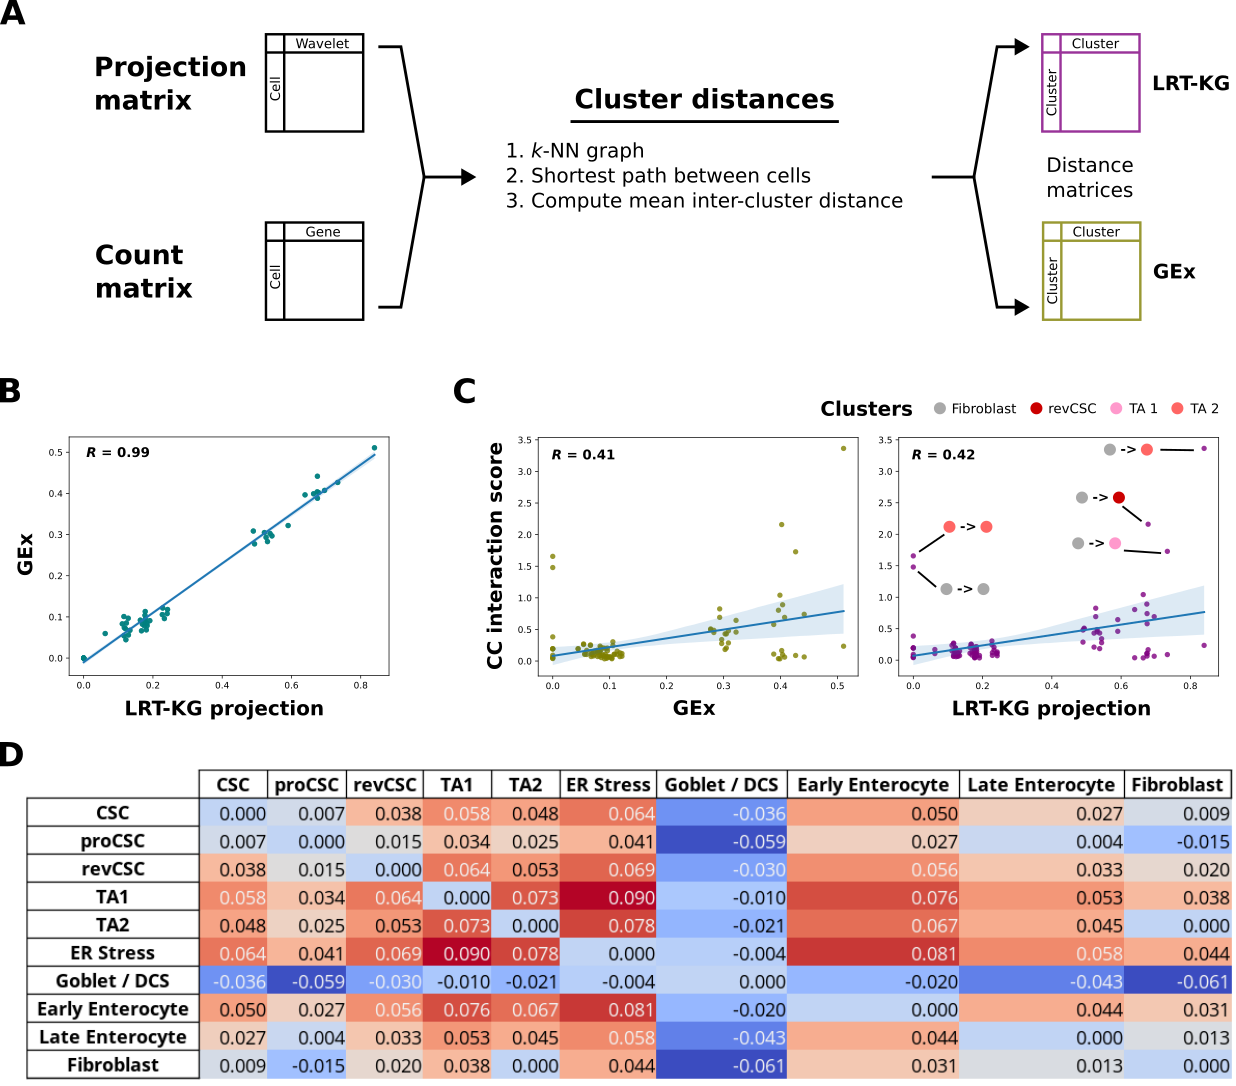
\includegraphics{06kg/figs/6KG_bench.png}
    \caption{XXXXXXXXXXXXX}
    \label{fig:6bench}
\end{figure}

\newpage
\section{Conclusions}

% * Built LRT KG that is comparable to other directed graphs in literature.
%     * IF omnpath capture ground bio truth, cell commns are indeed mostly hierarhcical. WE have a simplified hyper hierarhcical version.
% * KG embedding methods seem to conserve biological properties associted with nodes.
% * Wavelets used to difusse signal on graph so that single-cell \emph{omic} data can be projected on it.
% * Results match/conserve broader GEx information, but information gain is limited regarding cell communications.
% * Need to improve signal difussion step. Alternative gene embedding step can also be explored (GSP paper), so can the benchmarking be improved.


In this chapter I have assembled a knowledge graph for cell communication that captures relational information between ligands, receptors and downstream targets of transcriptional factors. The assembled LRT-KG is comparable in size and graph characteristics to the curated OmniPath database, albeit with a lower number of nodes but enhanced hierarchical structure due to the reductionist approach of limiting signalling flow into a single direction from secreting to receiving cells and the latter's intra-cellular responses. 

From this complex heterogeneous directed LRT-KG, methods like TransR can learn a lower-dimensional embedding that captures the original node characteristics of the graph and even biological information in the form of signalling pathways encoded in the relations between nodes. 
The resulting LRT-KG embedding is a relatively simple tabular representation of the cellular communications LRT-KG onto which we can project the transcriptomic profile of cells via wavelet diffusion.

Projection results revealed similar PHATE embeddings and high inter-cluster distance correlation between the gene expression and projection spaces, suggesting that the diffusion process within the graph is not of a sufficient degree and remains too reliant on the graph's nodes rather than on its structure. 
While the similarities with the \acrshort{gex} profile do validate the projection approach, and some degree of correlation between both spaces was expected, the lacking diffusion step results in the projected space being unable to differentially capture inter-cellular communications between the interacting stroma and epithelial compartment of WT organoid and fibroblast co-cultures.


% Given what we know on fibs interacting with revCSC and TA 2, I would expectd thos differences to be decreased on projected space, and at a mor macro level one might expect that cluster pairs displaying higher aggregate interaction probabilities (as determined by CellChat) should have present with shorter distances in the projected space when compared to the GEx space.


\chapter{Discussion and Future Perspectives}
\label{07disc}
\colorbox{yellow}{STLL WIP}

\section{Building Accessible and Automated Tools for MC Data Analysis}

In this work I have shown CyGNAL's capabilities, describing in detail its design and inner mechanisms, and outlining its usefulness with regards to the analysis of \acrshort{mc} datasets.

The main testament for the usefulness of the tool is the fact that it has become a part of routine \acrshort{mc} analyses in our lab. With its support for plain text to FCS inter-compatibility, one can seamlessly integrate with \acrshort{mc} platforms such as Cytobank. Additionally, as the user only need to run simple Python commands on the terminal to use CyGNAL, it has been readily adopted in day-to-day lab use even by users with no advanced computing experience. 
As I have shown in Chapters \ref{02methods} and \ref{03cytof}, CyGNAL is able to perform a comprehensive analysis of changes occurring across the samples of the often wide \acrshort{mc} experimental systems. Designed with a studying \acrshort{ptm} signalling changes in particular, CyGNAL's computation of \acrshort{emd} and \acrshort{dremi} scores resolves marker intensity and connectivity changes. The easy to use and customisable interactive Shiny-Apps allow for both exploratory and close to publication-grade visualisation of the results. Tools are meant to be used, and that publications by colleagues such as Michelozzi \textit{et al}.\cite{michelozzi_activation_2023} employed CyGNAL is a testament to its relevance.

Originally meant as a simple exercise in curiosity-driven exploration after noticing the correlation between so called PTM and 'cell-state' markers, and empowered by the tediousness of manually gating the datasets in our lab, the \acrshort{rf} cell-state classifier has become a convenient tool to automate cell-state labelling of \acrshort{mc} datasets in relation to cell-cycle phases.

Built around a simple \acrfull{rf} architecture, the \acrshort{rf} classifier benefits from the fundamental gate-like logic of both decision trees and the manual cell-state gating process. However, I expect the classifier to suffer from generalisation issues when dealing with external data labelled using different workflows. Furthermore, even if it leverages fuzzy logic to match channel names from the model to the input data, the classifier still relies on matching markers found in both the training data and the data to label. While the markers dedicated to apoptosis and cell-cycle phases generally belong to the less variable portions of \acrshort{mc} panel design, this can still pose an inconvenience when deploying the model. However, I have also shown how other weak points such as low performance for apoptotic class prediction using the 5-marker \acrshort{mc} model, can be effectively addressed by just the addition of an additional apoptotic marker to the panel design. Furthermore, the model seems resilient to cell-type composition and even to broad cell-state changes induced by chemotherapy.

Hearkening back to the link between \acrshort{ptm}s and cell-cycle, the 10-marker \acrshort{mc} model also reveals how certain \acrshort{ptm}s prove more informative when training than \emph{bona fide} cell-cycle markers, and discrepancies between expected state and \acrshort{ptm} correlations from the literature and feature importance rankings have anecdotally been used to validate under-performing antibodies with high unspecific background staining.

Both these tools remain relatively under continuous support, and the idea is to eventually merge both code bases and integrate automated cell-state classification into CyGNAL using pre-built classifier models or allowing for the generation of new models based on specific user-provided labelled data.
CyGNAL could also be augmented by the addition of PHATE~\cite{moon_visualizing_2019} as an alternative dimensionality reduction step, and implementing a third type of Shiny-App to visualise these embeddings and overlay user-selected metadata labels or antibody intensities.


\section{Charting Stromal and Oncogenic Regulation of CSC Polarisation}

Single-cell technologies can describe cell-cell communications and cell-type transitions in complex organoid settings and \emph{in vivo} tissues~\cite{qin_deciphering_2020, sqjin_sqjincellchat_2021, bues_deterministic_2022}. As shown in Qin \emph{et al.}~\cite{qin_cell-type-specific_2020}, a heterocellular colonic epithelia organoid system can be employed in experimental designs covering the effects of both intrinsic CRC oncogenic mutations and extrinsic cues. However, the directed and limited nature of the \acrshort{mc} antibody panels used in Qin \emph{et al.}~\cite{qin_cell-type-specific_2020} presented with a limiting factor towards detailed description of colonic organoid epithelial polarisation by intrinsic and extrinsic cues. 

Therefore, in Chapters \ref{04seq} and \ref{05vr} I have employed a multiplexed \acrshort{scrnaseq} analysis of heterocellular CRC organoid cultures to chart a continuous landscape of intrinsic and extrinsic regulation of colonic stem cell states. I have found that stromal cues transition the epithelia towards the \acrshort{revcsc} state, oncogenic signalling pushes the organoid towards \acrshort{procsc}, and exogenous ligands overlapping with both stromal and oncogenic signalling cues can polarise towards both states at once. I have also developed a method to capture these transitional processes, the \acrfull{vr} score, and established a workflow to project it onto Waddington-like data-driven landscapes. 
The work presented in this thesis was paired with complementary \emph{mc} experiments in Qin \& Cardoso Rodriguez \emph{et al.}~\cite{cardoso_rodriguez_single-cell_2023}, where we interrogated colonic stem cell regulation at scale to functionally understand the polarisation mechanisms (Appendix \ref{appendix:preprint}).

Here I have shown how the transcriptomic profiles of epithelial, fibroblast and macrophage cells from the heterocellular cultures can be used to describe inter-type heterogeneity and recapitulate the distinct epithelial compartments. 
The observed \emph{Cd34} high and low fibroblast populations are reminiscent of \emph{in situ} intestinal fibroblast heterogeneity, wherein \emph{Cd34} expressing fibroblast from the bottom of the crypts support the intestinal stem niche whereas \emph{Cd34} low fibroblast are found above the crypt's bottoms and help maintain the BMP gradient needed for epithelial differentiation. While we observed some transcriptional differences between these two fibroblast populations, their regulation of the epithelial compartment remained consistent, possibly due to shared TGF-\textbeta\hspace{0.1cm} between the two. 
Myeloid macrophage transcriptomes formed a continuum trajectory of putative inflammation-related roles, unlike the distinct fibroblast and epithelial populations. However, neither macrophages as a whole nor the extremes of their transcriptional continuum differentially regulated the epithelial cells.
The healthy small intestinal and colonic epithelia is supported by a stem cell niche at the bottom of the crypts regulated by both intrinsic and stroma-secreted signalling gradients. These traditional \acrfull{csc}s however, are not the sole stem cell state, with less common low-proliferative \acrfull{revcsc}s being able to replenish the \acrshort{csc} niche and repair the epithelial tissue in response to tissue damage~\cite{ayyaz_single-cell_2019}. Here I have shown how these \acrshort{revcsc} are enriched by stromal WNT and TGF-\textbeta\hspace{0.1cm} when WT organoids are co-cultured with fibroblasts, and how \acrshort{revcsc} also resemble public descriptions of the same population and a "foetal"-like state~\cite{mustata_identification_2013}.
The gradient of organoids with accumulating oncogenic mutations revealed how a \acrfull{procsc} state is enriched in CRC organoids. These cells are present in lower numbers in WT and \textit{shApc} organoids, but quickly dominate the landscape of stunted absorptive and secretory differentiation in the \textit{shApc} and \textit{Kras\textsuperscript{G12D/+}} (AK), and \textit{shApc}, \textit{Kras\textsuperscript{G12D/+}} and \textit{Trp53\textsuperscript{R172H/–}} (AKP) colonic organoids. \acrshort{procsc} were found to be transcriptionally similar to other cells from mouse models and human CRC.

With a clear differential regulation by extrinsic stromal cues and intrinsic oncogenic signalling, polarisation of WT colonic epithelia towards both \acrshort{procsc} and \acrshort{revcsc} could nonetheless be achieved via exogenous WENR added to the culture media. These findings, together with subsequent \acrshort{mc} validation~\cite{cardoso_rodriguez_single-cell_2023} of signalling hubs identified via cell-cell communication analysis, suggest that both states are part of a shared polarisation landscape with overlapping signalling hubs that overlap and compete with one-another to establish colonic epithelial cell-fate.
In this context, the observed breakdown of fibroblast-to epithelia communications in CRC organoids (at least partly due to downregulation of key signalling receptors by the epithelial cells) seems to suggest that intrinsic oncogenic cues dominate extrinsic stromal cues. The interplay between the two with regard to \acrshort{procsc} and \acrshort{revcsc} polarisation is explored further in Qin \& Cardoso Rodriguez \emph{et al.}~\cite{cardoso_rodriguez_single-cell_2023}, where we established that TGF-\textbeta\hspace{0.1cm} can induce \acrshort{revcsc}-like cells in CRC organoids in the context of low PI3K signalling, supporting the suggested role of \acrshort{revcsc} as a drug-resistant state in CRC that can drive relapse after chemotherapy~\cite{alvarez-varela_mex3a_2022, zapatero_trellis_2023}.

\emph{In silico} analysis of cellular dynamics has suggested that the epithelia transitions towards \acrshort{revcsc} following a polarisation processes from adjacent cell-sates, while \acrshort{procsc} dominance of the epithelia is achieved thanks to its proliferative potential.

I postulate that cellular pluripotency scores and rates of transcriptomic change capture the cellular dynamics of systems such as the colon epithelia, providing for an avenue towards generation of data-driven Waddington-like landscapes of cellular differentiation and plasticity. The \acrfull{vr} score described in Chapter \ref{05vr} synthesizes both CCAT and RNA velocity vector length metrics to capture coarse pluripotency changes and global transcriptomic structure thanks to PHATE. Finer details at a local level capture the availability of cell-sates on as determined by RNA velocity. Reconstruction of landscapes with ynthesis of processes as data-driven lasncapes representation. Powered by VR score, capture coarse pluripotency and transcriptomic strcuture. Local structure captures state avaialabiliyt as determined by RNA velocity.
Reconstructed landscapes recreated shared landscapes of polarisationand local transcriptomic. revcsc as an accesible state with stromal ligands, with oncocenic mtuations trapping the organoid in procsc.
    % When applied to murine organoid perturbation system described in Chapter \ref{04seq}, the VR landscapes depict a picture of a shared differentiation that can be traversed through cell-extrinsic ligands or cell-intrinsic oncogenic mutations. In particular, the increased availability of \acrshort{revcsc} in the presence of stromal ligands (Figure \ref{fig:4da}) can also be observed on the VR landscapes (Figure \ref{fig:5land}B). Furthermore, the collapse of stromal-to-epithelial communication in cancer organoids (Figure \ref{fig:4cc}A) and their lack of \acrshort{revcsc} polarisation (Figure \ref{fig:4da}C) is reflected in the tarn-like topology of the AK VR landscapes, where the bulk of the organoid appears trapped in the \acrshort{procsc} state.

Put together, these results describe fibros as master stromal regulators and CRC as a hyperproliferative trap. Given limitations of all organoid work and no insitu data, with no depe exploration of non paracrine stromal interactions or role of cafs. Further understanding triggering/blocking the rev and pro states necessary, specially as revcsc appear as a putative target to tackle emergence to chemoterapy resistance by blocking plasticity processes towards it. In terms of implemntation, increase accsibiliyt of VR landscapes by distributing it as an nbdev project, just like the pykrack package (Appendix \ref{appendix:pykrack}), but with interactive renderings of the generated landscapes. 


Last part discussing again relevance, revcsc as a baddie to target in cancer, and further understanding on triggering/blocking the rev and pro states necessary,specially regarding cafs, OF course also mention limitation of all organoid work, non paracrine effects, and with no in situ animal or human validation.
    % Our work and others now collectively suggest that fibroblasts are master regulators of revival stem cells in both the small intestine and colon.
    % Rather than establishing an entirely new cancer-specific cell-fate, our study suggests that oncogenic mutations cell-intrinsically polarise cells to an extreme yet pre-existing proCSC state, while simultaneously disrupting cell-extrinsic regulation of plasticity -- trapping cells as proCSC. These results describe cancer as a chronic, unidirectional shift in de-differentiation.
    % Collectively, our results and others suggest fibroblast-induced revCSCs may represent an important 'drug-tolerant persister' (DTP) state in CRC. Given that targeting cell-plasticity is an emerging area of cancer therapies \cite{burkhardt_mapping_2022}, future studies could target CRC DTP cells by combining YAP inhibitors (to block access to DTP revCSC) with standard chemotherapies (to kill proCSC). Helped by better understanding of caf effect Future cell-cell communication studies between CAF sub-types \cite{sahai_framework_2020} and defined epithelial genotypes could uncover exceptions to the signalling models described here and therefore provide novel avenues for therapeutic intervention in CRC.


\section{Knowledge Graph}

Coupled with emerging multimodal approaches that can capture at once intra and intercellular communication features, like phospho-seq \cite{blair_phospho-seq_2023} or Jamie's signal-seq. -> perfect tool to solve inter- and intra-cell communications at the single cell level without relying on clusters and in a modality agnostic way. 

Mixed results tbh.. Too similar to GEx and not good inverse correlation with cc probabilities (woudl expect cluster pairs highly interacting to have lowered distances [thus negative Pearson correlations]). Rsults sugest that diffusion step with wavelets is not enough, supported by work on prunned wavelt banks a larger scales and by projection on omnipath KG, which results in same GEx-like profile.

Fine balance between signal loss determined by lmited number of gene nodes on graph, but also on graph structure itself being important enough to produce results signficantly different from GEx matrix.



\phantomsection
\addcontentsline{toc}{chapter}{Appendices}

% The \appendix command resets the chapter counter, and changes the chapter numbering scheme to capital letters.
%\chapter{Appendices}
\appendix
\chapter{Appendix XXX}
\label{appendix:XXX}
(stuff)

\chapter{Cell-cycle Gene Lists}
\label{appendix:cycle}
Table of cell-cycle genes adapted from Tirosh et al. 2016 \cite{tirosh_dissecting_2016} and Macosko et al. 2015 \cite{macosko_highly_2015}, the former using a human melanoma cell line and the later both human and mouse models to link gene expression with cell cycle phases. The original tables provided in the publication were pooled together, duplicated genes were dropped, and human symbols were translated to mouse using BioMart. Finally, genes whose expression could not be deteced in any of the mouse organoid experiments were dropped from the list. The resulting table contains 98 genes associated with S-phase, 248 with both G2 and M-phase, and 202 with G1.

\begin{table}
  \centering
  \csvreader[
    tabular=|c|c|c|,
    table head=\hline \textbf{S-phase} & \textbf{G2 \& M-phase} & \textbf{G1} \\ \hline,
    late after line=\\ \hline,
    filter={\value{csvinputline}<44},
    separator=tab
  ]{0Xappendices/CellCycle_geneSet.txt}{}%
  {\csvcoli & \csvcolii & \csvcoliii}
  % \caption{Your table caption}
  \label{tab:your-table}
\end{table}
\begin{table}
  \centering
  \csvreader[
    tabular=|c|c|c|,
    table head=\hline \textbf{S-phase} & \textbf{G2 \& M-phase} & \textbf{G1} \\ \hline,
    late after line=\\ \hline,
    filter expr={
      test{\ifnumgreater{\thecsvinputline}{43}}
  and test{\ifnumless{\thecsvinputline}{86}}},
    separator=tab
  ]{0Xappendices/CellCycle_geneSet.txt}{}%
  {\csvcoli & \csvcolii & \csvcoliii}
  % \caption{Your table caption}
  \label{tab:your-table}
\end{table}
\begin{table}
  \centering
  \csvreader[
    tabular=|c|c|c|,
    table head=\hline \textbf{S-phase} & \textbf{G2 \& M-phase} & \textbf{G1} \\ \hline,
    late after line=\\ \hline,
    filter expr={
      test{\ifnumgreater{\thecsvinputline}{85}}
  and test{\ifnumless{\thecsvinputline}{128}}},
    separator=tab
  ]{0Xappendices/CellCycle_geneSet.txt}{}%
  {\csvcoli & \csvcolii & \csvcoliii}
  % \caption{Your table caption}
  \label{tab:your-table}
\end{table}
\begin{table}
  \centering
  \csvreader[
    tabular=|c|c|c|,
    table head=\hline \textbf{S-phase} & \textbf{G2 \& M-phase} & \textbf{G1} \\ \hline,
    late after line=\\ \hline,
    filter expr={
      test{\ifnumgreater{\thecsvinputline}{127}}
  and test{\ifnumless{\thecsvinputline}{170}}},
    separator=tab
  ]{0Xappendices/CellCycle_geneSet.txt}{}%
  {\csvcoli & \csvcolii & \csvcoliii}
  % \caption{Your table caption}
  \label{tab:your-table}
\end{table}
\begin{table}
  \centering
  \csvreader[
    tabular=|c|c|c|,
    table head=\hline \textbf{S-phase} & \textbf{G2 \& M-phase} & \textbf{G1} \\ \hline,
    late after line=\\ \hline,
    filter expr={
      test{\ifnumgreater{\thecsvinputline}{169}}
  and test{\ifnumless{\thecsvinputline}{212}}},
    separator=tab
  ]{0Xappendices/CellCycle_geneSet.txt}{}%
  {\csvcoli & \csvcolii & \csvcoliii}
  % \caption{Your table caption}
  \label{tab:your-table}
\end{table}
\begin{table}
  \centering
  \csvreader[
    tabular=|c|c|c|,
    table head=\hline \textbf{S-phase} & \textbf{G2 \& M-phase} & \textbf{G1} \\ \hline,
    late after line=\\ \hline,
    filter expr={
      test{\ifnumgreater{\thecsvinputline}{211}}},
    separator=tab
  ]{0Xappendices/CellCycle_geneSet.txt}{}%
  {\csvcoli & \csvcolii & \csvcoliii}
  % \caption{Your table caption}
  \label{tab:your-table}
\end{table}


\chapter{pyKrack}
\label{appendix:pykrack}

CAHpter on pykrack as a package. Concept of hierachy in a graph. Krackhadt heirahrcy. 

Implementaiotn in Python

Compare against already existing R implemtnation.
using nbdev for coding, vignettes, documentation, packaging and plublishing (to pypi).

Some kind of figure here

\section*{Introduction}

Biological signaling can be modeled as a directed network, where nodes represent genes/proteins and edges represent signaling interactions.

The hierarchy of such a network can be quantified using various metrics, including the Krackhardt hierarchy score. This score measures the degree to which the network exhibits a perfect hierarchy, with higher scores indicating greater hierarchy.

In R the sna package presents methods to compute graph hierarchy including Krackhardt’s score (defined as
where is the number of unordered pairs of points in Dr that are asymmetrically linked), and there are other hierarchy scores implemented in Python such as Flow Hierarchy Score Luo and Magee 2011. However, despite its utility, there is currently no native implementation of the Krackhardt hierarchy score in Python.

\subsection{}{Krackhardt hierarchy score}

As defined in Krackhardt, David. (1994). Graph Theoretical Dimensions of Informal Organization. Computational Organization Theory. 89.

The graph hierarchy condition states that in a digraph D, for each pair of points where one (Pi) can reach another (Pj), the second (Pj) can't reach the first (Pi). 
For example, in a formal organization chart a high lvl employee can reach through the chain of command her subordinate's subordinate. If the formal organization is working "properly", this lower lvl employee can't simultaneously reach the high lvl employee.
To measure the degree of hierarchy of digraph D, a new digraph Dr must be created. Dr is defined as the reachability digraph of D. Each point in D exists in Dr; moreover, the line (Pi,Pj) exists in Dr if and only if Pi can reach Pj in D. If D is graph hierarchic, then Dr will have no symmetric lines in it (i.e. if the line (Pi,Pj) exists in Dr then the line (Pj,Pi) does not).

The degree of hierarchy then is defined as:

Where is the number of unordered pairs of points in Dr that are symmetrically linked , and the number of unordered pairs of points in Dr where Pi is linked to Pj or viceversa.

%%%%%%%%

The Krackhardt hierarchy score is given by the following equation:

\begin{equation}
H_i = \frac{\sum_{j \in P_i} w_{ij} H_j}{k_i}
\end{equation}

where $H_i$ is the hierarchy score for node $i$, $P_i$ is the set of direct reports of node $i$, $w_{ij}$ is the weight of the edge between nodes $i$ and $j$, and $k_i$ is the number of direct reports of node $i$.

This equation calculates the hierarchy score for each node in a network based on the hierarchy scores of its direct reports and the weights of the edges between them. The hierarchy score represents the level of influence or power that a node has in the network, with higher scores indicating greater influence.





\section{Implementation}

\subsection{compute hierarchy function}

\subsection{nbdev paltform}


\chapter{Cell-state Random Forest Classifier}
\label{appendix:rfclass}

\section*{Rationale and Aims}

The maturity of the platform is also reflected on the properties of the markers used in the mass cytometry panels, with the most robust markers achieving highly binary and specific staining. Given the importance of cell state changes to perturbations in the epithelial organoids, either in the form of intrinsic effects such as genotype or extrinsic in the form of the TME or drug treatments, an automated approach of labelling and assigning a cell state to each cell in an experiment would facilitate routine analysis of mass cytometry datasets. 
I thus hypothesise that we can use a machine learning approach to, using a series of canonical cell state markers, automatically predict and label the hundreds of thousands of cells captured in a mass cytometry experiment. To this end I aim to develop a random-forest classifier. This classifier will be able to ingest mass cytometry datasets and, using manually gated datasets with cell state labels as training data, label each of the cells with one of six possible cell states: Apoptosis, G0, G1, S-phase, G2, and M-phase. 

\section*{Implementation}
The cell state classifier built uses the scikit-learn Python package35 to train and run a Random Forest classification algorithm. A Random Forest algorithm (referred to as RF hereafter) is based on a series of decision trees, simple non-parametric models that predict the class of an observation by learning decision rules inferred from the data during training. By using a randomised collection of these trees (i.e., a forest) the RF palliates the tendency of decision trees towards overfitness while at the same time reducing the variance of the results.

The current implementation in my personal GitHub repository (https://github.com/FerranC96/C\_StateML) consists of two scripts written in Python that are able to 1) train and save RF models from pre-labelled datasets, and generate classification reports and plots, 2) run the saved RF models through new mass cytometry datasets to label and assign a state to each cells. Default parameters are used for the Random Forest (except for an increase in the number of decision trees to 480) and the data is transformed as usual using an arcsinh function with a cofactor of 5. 

Some of the results presented in this document correspond to an initial implementation of the RF algorithm that used only 5 different cell state markers: pRB [S807/S811], cleaved Caspase 3 [D175], IdU, Cyclin B1, and pHH3 [S28]. This 5-marker implementation was trained using a balanced subset of cells from SI LGR5 time-course experiment in Qin et al. 202011 (downsampled so that all six cell states would have the same number of cells, 5306). The trained model was then tested against datasets from the same publication; a simpler single-timepoint SI LGR5 culture, and a complex coculture of colonic organoids (with varying degrees of CRC mutations and TME complexity).
In contrast, the latest results use data acquired from Patient Derived Organoids of CRC patients. With an updated panel, the markers used in the latest models are a set of ten antibodies (the five markers from above plus cPARP [D214], pAKT [T308], pP38 [T180/Y182], Geminin, and PLK1) with targets specific to each of the six cell state classes (Apoptosis, G0, G1, S-phase, G2, and M-phase). This 10-marker model was trained on an untreated control condition replicate and testing is performed against a second set of replicates comprising a total of 5 conditions (plus an untreated control) treated with increasing concentration of the chemotherapeutic topoisomerase inhibitor SN-38.
Details on the markers used in the RF models, and the cell state they are associated with, can be found in Sup. Table 1. To benchmark the model performance, we use F1-scores (calculated as the harmonic mean of the precision and recall for each class).

\section*{Results}

Testing the 5-marker RF model on a single time-point SI LGR5 organoid culture11 results in global accuracy for all classes of 0.93. However, looking at the classification report in Figure 3 a) we see how there is a significant drop of f1-scores when classifying the apoptotic class, scores which otherwise remain above 0.92. This fall in f1-scores seems to be driven by a low precision (0.5) when classifying cells as apoptotic.
Performance of the classifier drops when testing against the CRC TME colonic organoid cultures from Qin et al. 2020. In this case, when we subset just the organoid cells from the organoid cultures (i.e., by extracting all epithelial cells irrespective of the genotype or the other cell types they might have been analysed with), we observe a global accuracy of 0.91. Looking at the classification details (Figure 3 b.) we see a very similar pattern to the SI LGR5 results; with the apoptotic class presenting the lowest f1-scores (0.6) characterised by a low precision (0.43). Furthermore, the remaining f1-scores are also lower overall, with only the S-phase and M-phase classes reaching above the 0.9 mark.
When instead of subsetting just the organoid cells we test against all cells from the CRC TME dataset (i.e., including also fibroblasts and macrophages) global accuracy drops down to 0.87. The relatively high global accuracy does not reflect the failure of the classifier to, yet again, identify the apoptotic cells (see Figure 3 c.). In Figure 3 d) the classification matrix is used to build a dot plot in which the true labels (“Real state” from gating) are compared against the predicted labels (“Predicted state”), highlighting how a majority of the cells labelled as apoptotic are actually G0 cells, explaining the precision of 0.32 for the former class. There is also some confusion around the G2 cells, as a significant number of these cells are classified as either G0 or G1.
 
Figure 3: Benchmarking 5-marker RF cell state classifier. Shown in a), b), and c) are the classification reports obtained from running the 5-marker RF classifier against data manually labelled for cell state (representing the “real state” or ground truth). In a) a single timepoint SI LGR5 dataset was used, very similar to the training data for the model. The dataset in both b) and c) is a coculture of CRC organoids and their TME, with the cells in b) being a subset of the whole dataset containing just epithelial cells. Decreasing levels of performance correlate with increasing differences between the train and test datasets, as can be seen by the low f1-scores for the apoptotic class in c). Using the same data as c), the dot plot derived from the classification matrix in d) depicts the number and proportion (as both size and colour of the circles) of mislabelled cells for each cell state, showing that a considerable number of falsely mislabelled apoptotic cells are actually in G0 phase and some cells. RF: Random Forest.
Preliminary benchmark results from the updated 10-marker implementation using PDO data show improved performance when compared to the 5-marker model. In this case we observe a global accuracy greater than 0.99, with the lowest f1-score being of 0.95 for the cells in M-phase (see Figure 4 a.). In the classification matrix in Figure 4 b) we observe how, given the lower total count of M-phase cells (true label = 5, one order of magnitude smaller than the other classes), small numbers of misclassified cells (mainly as G2 and S-phase predicted labels, represented by the numbers 4 and 3 respectively) drive down the recall for the M-phase class. 
In contrast with the 5-marker model results, there is an apparent lack of issues when classifying the apoptotic class, with only 0.35% of true apoptotic cells being mislabelled. A bar plot representing the importance of each feature during classification is shown in Sup. Figure 2.
 
Figure 4: Benchmarking the new 10-marker RF cell state classifier. Building a RF classifier with an increased number of markers using data from PDOs renders better results than the original 5-marker model, as can be seen in a) with the classification report. b) Classification matrix generated automatically during model building, showing extremely low levels of misclassified cells. RF: Random Forest. PDO: Patient-Derived Organoids. Labels: 0=Apoptosis, 1=G0, 2=G1, 3=S-phase, 4=G2, 5=M-phase.


\section*{Discussion}
This classifier shows link PTM->cellSTate, later shown in pubs from our lab
Usefullness in determining antibodies not working properly?


\chapter{Appendix CardosoRodriguez \& Qin et al.}
\label{appendix:XXX}

\includepdf[pages=-, scale=1, offset=24mm -28mm]{0Xappendices/preprint.pdf}



\chapter{Colophon}
\label{appendix3label}
\textit{This is a description of the tools you used to make your thesis. It helps people make future documents, reminds you, and looks good.}

\textit{(example)} This document was set in the Times Roman typeface using \LaTeX\ and Bib\TeX , composed with a text editor. 
 % description of document, e.g. type faces, TeX used, TeXmaker, packages and things used for figures. Like a computational details section.
% e.g. http://tex.stackexchange.com/questions/63468/what-is-best-way-to-mention-that-a-document-has-been-typeset-with-tex#63503

% Side note:
%http://tex.stackexchange.com/questions/1319/showcase-of-beautiful-typography-done-in-tex-friends

% You could separate these out into different files if you have
%  particularly large appendices.

% Actually generates your bibliography. The fact that \include is 
% the last thing before this ensures that it is on a clear page.
\bibliography{references}

% All done. \o/
\end{document}














































































